% !TEX program = xelatex
% 为什么学线性回归（Why Linear Regression）——中文教程
% 作者：熊昊一 (Haoyi Xiong)
\documentclass[11pt, a4paper]{ctexart}

% ---------- 中文字体 ----------
\usepackage{xeCJK}
\setCJKmainfont{PingFang SC}
\setCJKsansfont{PingFang SC}

% ---------- 数学 ----------
\usepackage{amsmath, amssymb, amsthm, mathtools}
\usepackage{bm}
\usepackage{geometry}
\geometry{margin=2.5cm}

% ---------- 排版 ----------
\usepackage{microtype}
\usepackage{enumitem}
\usepackage{booktabs}
\usepackage{xcolor}
\definecolor{accent}{RGB}{0, 90, 160}
\definecolor{lightband}{RGB}{240, 244, 248}
\usepackage{tcolorbox}
\tcbuselibrary{breakable, skins}
\usepackage{graphicx}
\usepackage{tikz}
\usetikzlibrary{arrows.meta, calc, positioning}
\usepackage{hyperref}
\hypersetup{
  colorlinks=true,
  linkcolor=accent,
  citecolor=accent,
  urlcolor=accent,
  pdftitle={Why (we still need) linear regression -- a deep-dive for applied and data scientists},
  pdfauthor={Haoyi Xiong, Lingkai Kong},
}

% ---------- 定理环境（中文名） ----------
\theoremstyle{plain}
\newtheorem{theorem}{定理}[section]
\newtheorem{lemma}[theorem]{引理}
\newtheorem{corollary}[theorem]{推论}
\theoremstyle{definition}
\newtheorem{definition}[theorem]{定义}
\newtheorem{example}[theorem]{例}
\newtheorem{exercise}{练习}[section]
\theoremstyle{remark}
\newtheorem*{remark}{注}
\newtheorem*{intuition}{直观}

% ---------- 强调框 ----------
\newtcolorbox{keybox}[1][]{
  colback=lightband, colframe=accent, fonttitle=\bfseries,
  title={#1}, breakable, sharp corners, boxrule=0.6pt, left=2mm, right=2mm, top=1.5mm, bottom=1.5mm
}

% ---------- 常用宏 ----------
\newcommand{\R}{\mathbb{R}}
\newcommand{\E}{\mathbb{E}}
\newcommand{\Prob}{\mathbb{P}}
\newcommand{\Var}{\mathrm{Var}}
\newcommand{\Cov}{\mathrm{Cov}}
\newcommand{\rank}{\mathrm{rank}}
\newcommand{\trace}{\mathrm{tr}}
\newcommand{\MSE}{\mathrm{MSE}}
\newcommand{\X}{\mathbf{X}}
\newcommand{\y}{\mathbf{y}}
\newcommand{\bhat}{\widehat{\bm{\beta}}}
\newcommand{\bbeta}{\bm{\beta}}
\newcommand{\x}{\mathbf{x}}
\newcommand{\zero}{\mathbf{0}}
\newcommand{\norm}[1]{\left\lVert #1 \right\rVert}
\newcommand{\relu}[1]{\mathrm{ReLU}\!\left(#1\right)}
\newcommand{\ind}[1]{\mathbf{1}\!\left\{#1\right\}}

\title{\Huge \textbf{Why (we still need) linear regression}\\[6pt]
\Large a deep-dive for applied and data scientists\\[10pt]
\large 为什么（依然）需要线性回归 --- 写给应用与数据科学家的深度教程}
\author{Haoyi Xiong (熊昊一) \and Lingkai Kong (孔令凯)}
\date{\today}

\begin{document}

\maketitle

\begin{abstract}
\noindent
线性回归是所有人第一个学、也几乎被所有人低估的模型。
这篇教程不谈如何在 R 里跑 \texttt{lm()}、在 scikit-learn 里调 \texttt{LinearRegression()}——它回答的是\textit{为什么}这个方法有效：为什么平方误差、为什么正规方程、为什么相关系数出现在回归系数里、为什么一条直线既能度量\textit{相关性}却不能断言\textit{因果性}，以及为什么在两百多年后，一个$d$维的超平面公式
$\widehat{\bm{\beta}} = (\X^\top \X)^{-1} \X^\top \y$
仍然是数据分析最诚实的起点。
全文只需高中微积分与基础线性代数，所有结论都从头推导，并附有可查证的历史文献。
\end{abstract}

\newpage
\tableofcontents
\newpage

% 前言
\section*{前言}\label{sec:preface}
\addcontentsline{toc}{section}{前言}

\subsection*{这本书写给谁}

这本教程写给\textbf{有一定数学基础的 applied scientists 和 data scientists}——你学过线性代数和微积分，日常用 \texttt{lm()}、\texttt{LinearRegression()} 或 \texttt{np.linalg.lstsq} 解决实际问题，但隐隐觉得「会用」和「理解」之间隔着一层窗户纸：为什么斜率恰好是相关系数？为什么平方损失而不是绝对值？$d > n$ 时训练误差为零的模型凭什么能泛化？核方法和我的线性回归是什么关系？

如果你有这样的疑问，这本书就是为你写的。它不教你调包（那是文档的工作），它把每一个公式从头推给你看，并告诉你每个定理背后的\textbf{假设清单}——因为假设才是统计学的本体，公式只是影子。全文只需本科程度的微积分与线性代数加基础概率；所有结论都可从头验证，书末附有全部习题的完整解答。

\subsection*{缘起与影响}

这本书的写作是\textbf{一时兴起}——某个晚上，作者想把脑子里盘了很久的「为什么学线性回归」一口气写出来，于是一章一章写到了第 8 章。但它的「兴」背后，是长期阅读一批科学家工作的积累。七位影响最深的学者是：\textbf{Francis Bach}（Inria），他的教科书 \emph{Learning Theory from First Principles}（2024）\cite{bach2024} 与本书「每个结果都从第一性原理挣出来」的气质一脉相承，第 \ref{sec:kernel} 章的核方法视角与第 \ref{sec:gd}--\ref{sec:gd-underdet} 章优化--统计互通的写法都受其影响；\textbf{Ryan Tibshirani}（斯坦福大学），他把 generalized lasso、trend filtering、conformal prediction 做成了「既可计算、又可审计」的方法论，这正是本书第 \ref{sec:ggm} 章 estimate-to-inference 路线的精神；\textbf{Jingfeng Wu}（UC Berkeley Simons Institute），他关于「gradient descent dominates ridge regression」的工作\cite{wu2025}正是本书第 \ref{sec:gd}--\ref{sec:implicit} 章迭代--正则化故事的统计学前沿；\textbf{Arthur Jacot}（纽约大学 Courant 研究所），他提出的神经正切核（NTK）\cite{jacot2018} 把「线性回归 $\to$ 核回归 $\to$ 深度网络」焊成了一条完整的路，即本书第 \ref{sec:ntk} 节；\textbf{Jianqing Fan}（普林斯顿大学），他的高维统计体系\cite{fan2020}——稀疏估计、变量筛选、大协方差矩阵——是本书第 \ref{sec:ggm} 章从估计到推断这条路线图的来源；\textbf{David Donoho}（斯坦福大学），压缩感知（compressed sensing）的奠基人，他证明 $\ell_1$ 极小化能以最优方式利用稀疏性、欠定方程组在稀疏假设下可解\cite{donoho2006}——本书第 \ref{sec:sparsity} 节「稀疏性是可计算的假设」正是这一思想的统计学表达；\textbf{Emmanuel Candès}（斯坦福大学），与 Donoho、Tao 共创压缩感知的精确恢复理论，又以 knockoffs 框架给出了复杂模型下可复现的变量选择与错误发现率（FDR）控制\cite{barber2015}——这是本书第 \ref{sec:debiased} 节「点估计如何升级为可检验的推断」之后的现代下一站。

\subsection*{写作方式与一份诚实的免责声明}

\textbf{这本书大量使用了 AI 辅助写作。} 具体而言，正文由 Moonshot AI 的 Kimi K2.8 模型在 \textbf{Kimi Work 桌面版}的 Agent 模式下完成——由它直接编写 LaTeX 源码、编译 PDF、渲染检查、逐页校对；人类专家（Haoyi Xiong）给出 outline、章节内容与自己的思考，尤其是他对线性回归多年的理解、以及他自己曾专门研究过的几个点（如欠定情形梯度下降的精确解、latent 投影下的核方法视角、精度矩阵与条件独立的联系）。一句话分工：\textit{人类负责「问什么」和「信不信」，机器负责「写出来」和「查出来」}。

因此请读者注意以下三点：

\begin{enumerate}[label=(\alph*)]
  \item \textbf{线性回归这个领域非常大}，本书没有、也不可能覆盖全部：广义线性模型、稳健回归、混合效应模型、时间序列、贝叶斯路线、在线学习、联邦场景……每一样都配得上自己的一本 deep-dive。本书只覆盖作者认为「不答就不诚实」的那条主线。
  \item \textbf{本书的理论部分并不追求专业严格}。所有公式都正确、可推导，但证明显然不是教科书级别的完备（比如渐近结果的正则条件一律从略）。\textit{做理论研究的读者请跳过本书}；初学或没系统接触过的读者，可以把它当作一份有推导的科普放心阅读。
  \item \textbf{历史与文献部分尽力核实}（主要人物、年份与出处均经联网查证并在参考文献中标注），但若有讹误，责任在人类作者，欢迎指正。
\end{enumerate}

先拟合直线，审计假设，诚实披露弱点——这本书自己也照此办理。

\vspace{1em}
\hfill 熊昊一 (Haoyi Xiong)，于北京


\clearpage
% 第 1 章
\section{引言：为什么两百年后，直线仍是诚实数据分析的起点}\label{sec:intro}

\subsection{这篇教程要回答的问题}

每一门机器学习课程、每一本统计教材，都会在头两周讲线性回归；而它们几乎都以同样的方式讲：扔给你一个公式
\[
  \widehat{\bm{\beta}} = (\X^\top \X)^{-1} \X^\top \y,
\]
让你记住，然后赶紧奔向「更激动人心」的模型。

这篇教程反着来：每一步都自己挣出来。读完之后，你应该能从第一性原理回答：

\begin{enumerate}[label=(\arabic*)]
  \item 为什么一维回归的斜率是 $\dfrac{\Cov(x,y)}{\Var(x)}$？它和 Pearson 相关系数到底是什么关系？（第 \ref{sec:onedim} 章）
  \item 为什么一条直线能量出 $x$ 与 $y$ 的\textit{相关性}，却不能告诉你因果的\textit{方向}？（第 \ref{sec:onedim} 章）
  \item 为什么平方误差？换别的损失会丢掉什么？（第 \ref{sec:why-square} 节）
  \item 高维情形下，当样本量 $n$ 远大于维度 $d$ 时，为什么最小二乘有闭式解 $\widehat{\bm{\beta}} = (\X^\top\X)^{-1}\X^\top\y$？这个解何时唯一、何时最优？（第 \ref{sec:highdim} 章）
  \item 当 $n$ 不再远大于 $d$ 时，是什么先坏掉，修复又是什么？（第 \ref{sec:hd-break} 节）
  \item 把闭式解与梯度下降迭代放在一起，$\widehat{\bm{\beta}}_t$ 有怎样的精确解？不动点意味着什么？（第 \ref{sec:gd} 章）
  \item 当 $d > n$、解已成流形时，迭代收敛到哪里？它与伪逆解是什么关系？（第 \ref{sec:gd-underdet} 章）
  \item 回归系数与协方差、精度矩阵是什么关系？「估计」如何升级为「推断」——即 from estimate to inference？（第 \ref{sec:ggm} 章）
  \item 当观测特征其实是潜变量的非线性投影时，线性回归为何表现为一个核方法？（第 \ref{sec:kernel} 章）
\end{enumerate}

\subsection{一个两百岁、拒绝退休的想法}

最小二乘法由 Legendre（1805）首次发表，Gauss（1809）独立提出并从概率论角度给出了完整推导——后者用它从有噪声的天文观测中预测了谷神星（Ceres）的轨道\cite{legendre1805,gauss1809}。这个方法熬过了此后每一次范式更替：计算机、自助法（bootstrap）、深度学习革命。原因只有一个：

\begin{keybox}[本教程的论点]
线性回归流行，不是因为现实世界是线性的——它很少是。它流行是因为：
\begin{enumerate}[label=(\roman*)]
  \item 局部线性近似常常足够好（Taylor 定理保证了任何光滑函数在局部都是近线性的）；
  \item 它是\textit{唯一可精确求解、可解释、可审计}的基线——其余一切模型都是对照它来衡量自己的；
  \item 它是 logistic 回归、广义线性模型、核方法乃至神经网络输出层的地基。
\end{enumerate}
\end{keybox}

\begin{figure}[htbp]
  \centering
  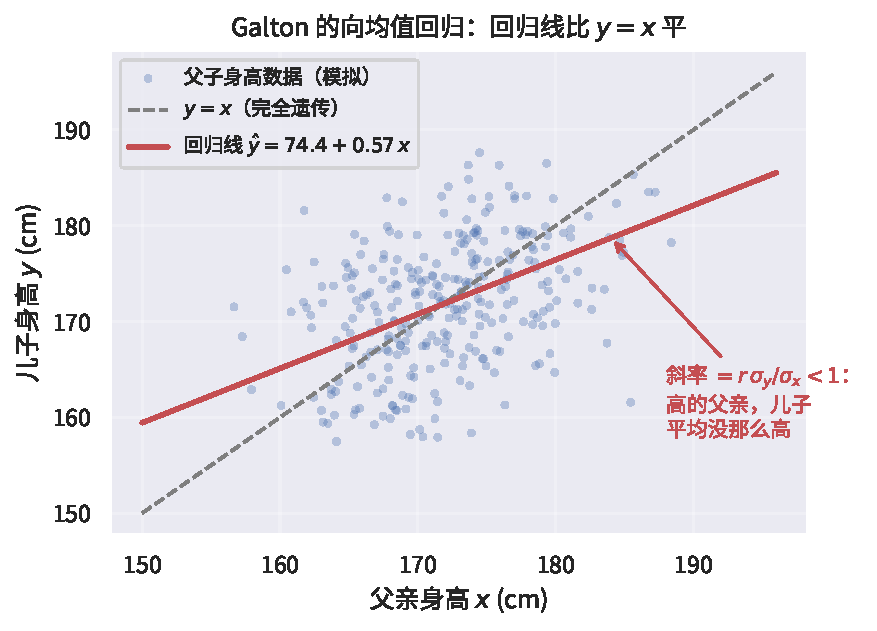
\includegraphics[width=0.8\linewidth]{figures/ch1_galton.pdf}
  \caption{Galton 的「向均值回归」（模拟数据重现）：回归线（红）始终比 $y=x$（灰虚线）平——斜率 $=r\,\sigma_y/\sigma_x$，只要 $|r|<1$，极端必然后退。两百年后，这条直线仍是数据分析的默认起点。}
  \label{fig:ch1-galton}
\end{figure}

\subsection{预备知识}

\begin{itemize}
  \item \textbf{微积分}：偏导数、链式法则，以及「光滑函数的极值出现在导数为零处」这一事实；
  \item \textbf{线性代数}：向量、矩阵、矩阵乘法、转置、逆；「矩阵乘向量是列的线性组合」这一读法；
  \item \textbf{概率}（第 2 章用到）：期望、方差、协方差、相关系数。
\end{itemize}

其余皆在文中推导。

\subsection{记号，只说一次}

一维情形：$n$ 对观测 $(x_i, y_i) \in \R^2$，$i = 1, \dots, n$。高维情形：响应 $y_i \in \R$，特征 $\x_i = (x_{i1}, \dots, x_{id})^\top \in \R^d$，设计矩阵 $\X \in \R^{n \times d}$（行为 $\x_i^\top$），参数 $\bbeta \in \R^d$。误差项 $\varepsilon_i$ 收纳一切直线解释不了的东西：测量噪声、遗漏的变量、真实的随机性，以及「用超平面近似非线性世界」这一罪过本身。

约定：
\[
  \bar{x} = \frac{1}{n}\sum_{i=1}^n x_i, \qquad
  \Var_n(x) = \frac{1}{n}\sum_{i=1}^n (x_i - \bar{x})^2, \qquad
  \Cov_n(x, y) = \frac{1}{n}\sum_{i=1}^n (x_i - \bar{x})(y_i - \bar{y}),
\]
即以 $n$ 为分母的样本方差与协方差（用 $n-1$ 只会给比值带来一个无关紧要的因子）。全程用 $\Var$、$\Cov$ 表示对随机变量取期望的总体量，用下标 $n$ 表示样本量。

\clearpage
% 第 2 章
\section{一维线性回归：一条直线里的相关性、方向与因果}\label{sec:onedim}

从最简模型出发——没有截距、只有一个特征：
\begin{equation}\label{eq:1d-model}
  y_i = b\, x_i + \varepsilon_i, \qquad i = 1, \dots, n,
\end{equation}
其中 $b \in \R$ 是待估参数。这一章做两件事：先\textit{从回归的角度}看 $b$ 如何度量 $x$ 与 $y$ 的相关性；再\textit{从方差的角度}看同一条直线如何暴露相关性的\textit{方向性}，以及为什么它不能告诉你因果。

\subsection{最小二乘：把均值推广成一条线}\label{sec:1d-ls}

先忘记统计。把拟合问题写成优化问题：找 $b$，让残差平方和
\begin{equation}\label{eq:1d-rss}
  S(b) = \sum_{i=1}^n (y_i - b\, x_i)^2
\end{equation}
最小。对 $b$ 求导并令其为零：
\[
  \frac{dS}{db} = -2 \sum_{i=1}^n x_i (y_i - b x_i) = 0
  \quad\Longrightarrow\quad
  \boxed{\;\hat{b} = \frac{\sum_{i=1}^n x_i y_i}{\sum_{i=1}^n x_i^2}\;}
\]
二阶导数 $\frac{d^2 S}{db^2} = 2 \sum_i x_i^2 > 0$（只要 $x$ 不全为零），故这是唯一的全局最小值点。没有初值、没有学习率、没有局部极小值——凸性一次性解决。

先看两个极端，建立直觉。若 $x_i \equiv 1$，$\hat{b} = \bar{y}$：\textbf{最小二乘是均值的推广}，样本均值正是使平方偏差最小的那个常数。若模型有截距 $y_i = a + b x_i + \varepsilon_i$，完全一样的求导给出
\begin{equation}\label{eq:1d-slope}
  \hat{b} = \frac{\Cov_n(x, y)}{\Var_n(x)}, \qquad \hat{a} = \bar{y} - \hat{b}\,\bar{x},
\end{equation}
即回归线必过数据中心点 $(\bar{x}, \bar{y})$。请把 \eqref{eq:1d-slope} 慢慢读一遍：\textit{斜率 = $x$ 与 $y$ 一起变化的程度，除以 $x$ 自身变化的程度}。整个应用统计学中被引用最多的公式，不过是一次求导的结果。注意此时还没有假设任何误差分布——最小二乘到目前为止纯粹是几何优化。

\subsection{回归视角：斜率就是相关系数}\label{sec:1d-corr}

现在把数据标准化。记 $\sigma_x = \sqrt{\Var_n(x)}$，$\sigma_y = \sqrt{\Var_n(y)}$，Pearson（1896）相关系数\cite{pearson1896}为
\begin{equation}\label{eq:rho}
  r = \frac{\Cov_n(x, y)}{\sigma_x \, \sigma_y} \in [-1, 1].
\end{equation}
（由 Cauchy--Schwarz 不等式 $|\Cov_n(x,y)| \le \sigma_x \sigma_y$ 可知 $r$ 确实落在 $[-1,1]$。）代入 \eqref{eq:1d-slope}：
\begin{equation}\label{eq:slope-rho}
  \boxed{\;\hat{b} = r \, \frac{\sigma_y}{\sigma_x}\;}
\end{equation}

这一行是全章的枢纽，它说三件事：

\begin{enumerate}[label=(\arabic*)]
  \item \textbf{相关的\textit{强度}}（$|r|$，无量纲、对称、与单位无关）决定回归线的\textit{陡度}（以标准差为单位）：$\frac{\hat{b}\, \sigma_x}{\sigma_y} = r$。把 $x$ 移动一个标准差，预测 $\hat{y}$ 移动 $r$ 个标准差。
  \item \textbf{$r$ 的对称性 vs.\ 回归的方向性}：$r$ 对换 $x$、$y$ 不变；但回归线 $y \sim x$（以 $x$ 预测 $y$）与回归线 $x \sim y$ 是两条\textit{不同}的线（见 \ref{sec:1d-direction} 节）。
  \item \textbf{拟合优度}：判定系数
  \begin{equation}\label{eq:r2-rho2}
    R^2 = 1 - \frac{\sum_i e_i^2}{\sum_i (y_i - \bar{y})^2} = r^2,
  \end{equation}
  即「$y$ 的样本方差中被 $x$ 线性解释的比例」恰好是相关系数的平方。$R^2$ 度量相关性，而 $r$ 还带有符号（方向）。
\end{enumerate}

\begin{example}[Galton 的身高回归]\label{ex:galton}
Galton（1886）研究 205 对父母与 928 名成年子女的身高，以「中亲身高」$x$ 预测子代身高 $y$，得到的回归方程约为 $y = 0.516\,x + 33.73$（英寸）\cite{galton1886}。两代人的标准差几乎相同（约 3.3 英寸），于是以标准差计的斜率就是 $r \approx 0.5$：父母比平均值高一个标准差，子女平均只高半个标准差。高个父母的子女\textbf{趋向平庸}，矮个父母的子女同样趋向平庸——「回归均值」（regression toward the mean）由此得名。这不是生物学的规律，是 \eqref{eq:slope-rho} 的算术：只要 $|r| < 1$ 且两变量各自散布稳定，极端必然后退。\end{example}

\begin{remark}
「回归均值」是统计误用之祖：体育画报魔咒、第二次考试退步、《商业平庸的胜利》（Secrist, 1933）之流的「论证」，本质都是把噪声当作了规律。Galton 本人则用更精细的论证避开了这个陷阱\cite{galton1886,stigler1986}。
\end{remark}

\begin{figure}[htbp]
  \centering
  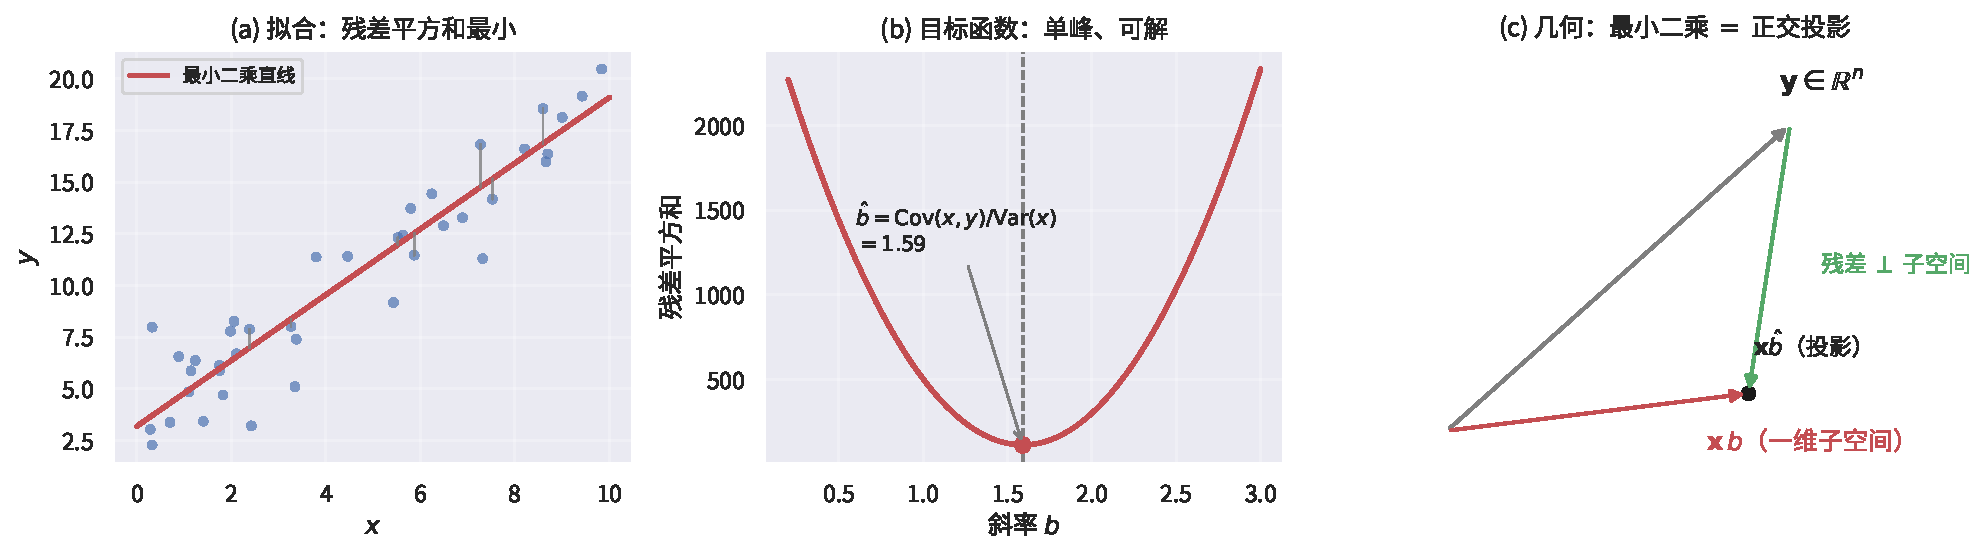
\includegraphics[width=\linewidth]{figures/ch2_leastsq.pdf}
  \caption{一维最小二乘的三个侧面：(a) 拟合——残差（竖线）平方和最小；(b) 优化——目标函数对斜率 $b$ 单峰，$\hat b=\Cov(x,y)/\Var(x)$ 可一步解出；(c) 几何——$\x\hat b$ 是 $\y$ 在一维子空间上的正交投影，残差 $\perp$ 子空间。}
  \label{fig:ch2-leastsq}
\end{figure}

\subsection{方差视角：相关从哪里来，又意味着什么}\label{sec:1d-var}

换一种眼光。把 \eqref{eq:1d-model} 中的 $y$ 看成随机变量 $y = bx + \varepsilon$，假设 $\Cov(x, \varepsilon) = 0$（即 $x$ 中不含 $y$ 的噪声成分——这本身就是一个方向性假设！）。方差的代数给出
\begin{equation}\label{eq:var-decomp}
  \Var(y) = b^2 \Var(x) + \Var(\varepsilon).
\end{equation}
\textbf{$y$ 的波动被拆成两部分：由 $x$ 携带的部分 $b^2\Var(x)$，和无法归约的噪声 $\Var(\varepsilon)$。}立刻得到
\begin{equation}\label{eq:r2-var}
  R^2 = \frac{b^2 \Var(x)}{\Var(y)} = 1 - \frac{\Var(\varepsilon)}{\Var(y)},
\end{equation}
与 \eqref{eq:r2-rho2} 殊途同归：$r^2$ 既是「样本层面拟合优度」，又是「总体层面被解释的方差占比」。这就是用方差视角看回归的第一个收获——\textit{相关性的实质，是方差的转移}。

第二个收获更深。\eqref{eq:var-decomp} 里 $b$ 的方向（正负）描述的是「$x$ 的波动如何翻译成 $y$ 的波动」。若真实结构其实是 $y$ 导致 $x$，仍按 $y \sim x$ 回归，得到的仍是同一个 $\hat{b} \approx r\,\sigma_y/\sigma_x$。相关性对生成方向\textit{完全盲视}——这是下一节的主旨。

\subsection{方向性：两条回归线，与一条主轴}\label{sec:1d-direction}

把 $x$、$y$ 都标准化（均值为 0、方差为 1），则两个方向的\textbf{回归系数}都等于 $r$：
\[
  \text{回归 } y \sim x \text{ 的系数} = r,
  \qquad
  \text{回归 } x \sim y \text{ 的系数} = r,
  \qquad
  \text{两系数之积} = r^2 < 1 \; (|r| < 1).
\]
（第二个等号是「系数」而非「斜率」：$x \sim y$ 回归解出的是 $x = r\,y$，把 $y$ 当自变量读，系数确实是 $r$。）也就是说，除非 $|r| = 1$（完全线性，无噪声），\textbf{「用 $x$ 预测 $y$ 的线」与「用 $y$ 预测 $x$ 的线」是两条不同的直线}。这里有一个必须说清的口径问题：\textit{回归系数}与\textit{画在同一坐标系里的几何斜率}不是一回事。原始尺度上两条线的回归系数分别是
\[
  b = r\,\frac{\sigma_y}{\sigma_x} \;(y \sim x), \qquad
  b' = r\,\frac{\sigma_x}{\sigma_y} \;(x \sim y),
  \qquad b\, b' = r^2 < 1,
\]
——系数之积是 $r^2$，这是 Galton「回归均值」的算术；但若把两条线都画在「$x$ 横轴、$y$ 纵轴」的同一坐标系里，第二条线要改写成 $y = \dfrac{\sigma_y}{r\,\sigma_x}\,x$，\textbf{几何斜率}分别为 $r\,\sigma_y/\sigma_x$ 与 $\sigma_y/(r\,\sigma_x)$，乘积恒为 $1$。两个乘积都对，只是度量了两个不同的问题：前者问「两个方向的预测各收缩多少」，后者问「两条直线在图上的张角」。点云近似一个椭圆（二元正态的样子），两条回归线分别是：竖直残差最小的线与水平残差最小的线——都不是椭圆的主轴（主轴对应 PCA，要求\textit{垂直}距离最小）。把图 \ref{fig:ellipse} 看进脑子里，「回归有方向、相关没有」就不再是口号。

\begin{figure}[htbp]
\centering
\resizebox{0.72\linewidth}{!}{%
\begin{tikzpicture}[>=Stealth, scale=2.6]
  % 点云椭圆
  \draw[thick, color=black!60, rotate around={35:(0,0)}] (0,0) ellipse (2.2 and 1.0);
  \fill[black!40] (35:1.3) circle (0.02);
  \fill[black!40] (215:0.9) circle (0.02);
  \fill[black!40] (35:-0.8) circle (0.02);
  \fill[black!40] (215:1.6) circle (0.02);
  \fill[black!40] (35:0.3) circle (0.02);
  \fill[black!40] (215:-1.4) circle (0.02);
  \draw[->] (-2.9,0) -- (2.9,0) node[below left] {$x$};
  \draw[->] (0,-2.3) -- (0,2.3) node[below left] {$y$};
  % 主轴
  \draw[thick, dashed, color=black!50] (-2.35,-1.65) -- (2.35,1.65) node[above right=-2pt] {主轴（PCA）};
  % 回归线 y~x: 斜率 tan(35°) * (短轴/长轴) ≈ 0.7*0.455 ≈ 0.32 → 用 rotate 近似
  \draw[very thick, color=accent] (-2.7,-0.86) -- (2.7,0.86) node[below right=-2pt] {回归 $y \sim x$};
  % 回归线 x~y
  \draw[very thick, color=red!70!black] (-1.35,-2.2) -- (1.35,2.2) node[above=-2pt] {回归 $x \sim y$};
\end{tikzpicture}}
\caption{标准化后的二元正态点云（椭圆）。两条回归线都不重合于主轴：$y \sim x$ 最小化竖直残差，$x \sim y$ 最小化水平残差，主轴最小化垂直残差。回归是\textit{有方向}的运算，相关系数 $r$ 则没有。}
\label{fig:ellipse}
\end{figure}

方向性还有一个纯代数的表述：\eqref{eq:var-decomp} 的分解 $\Var(y) = b^2\Var(x) + \Var(\varepsilon)$ 与 $\Var(x) = \tilde{b}^2 \Var(y) + \Var(\tilde\varepsilon)$（$x$ 对 $y$ 回归）可以同时成立，且各自的 $R^2$ 都是 $r^2$。两个方向「解释力」相同，这正是相关性对称性的方差表达；而斜率不同，则是方向性的表达。

\subsection{因果性：相关系数永远给不出的东西}\label{sec:1d-causality}

为什么 $r$ 不能断言因果？因为至少三种截然不同的生成机制，产生\textit{完全相同}的相关系数：

\begin{center}
\begin{tabular}{@{}lll@{}}
\toprule
结构 & 生成方式 & 观测到的相关 \\
\midrule
$x$ 导致 $y$ & $y = bx + \varepsilon$ & $r \neq 0$ \\
$y$ 导致 $x$ & $x = \tilde{b} y + \tilde\varepsilon$ & $r \neq 0$（同一个 $r$） \\
共同原因 $z$ & $x = c z + u,\;\; y = d z + v$ & $r = \mathrm{sign}(cd)\cdot(\text{由 } c,d \text{ 决定})$ \\
\bottomrule
\end{tabular}
\end{center}

数据本身对这三种情形零区分能力——这是 Reichenbach（1956）\textbf{共同原因原理}的推论：若 $A$、$B$ 统计相关，则要么 $A$ 导致 $B$，要么 $B$ 导致 $A$，要么存在共同原因 $C$\cite{reichenbach1956}。原理给出了枚举，却没有给出判别——判别必须借助数据之外的知识。

Wright（1921）是第一个把这件事做成演算的人\cite{wright1921}。他的\textbf{路径分析}说：在一张给定的因果图（箭头必须从实验、时序或领域知识中事先画出）上，任意两变量的相关系数等于连接它们的所有合法路径上系数乘积之和。于是：
\begin{itemize}
  \item \textit{正向使用}：给定因果假设，用观测到的相关去\textit{检验}它（拟合、残差相关应为零）；
  \item \textit{反向使用}：从相关反推因果结构，统计学本身无能为力——「这些结论的正确性取决于方法之外的知识」（Wright 原文的意思\cite{wright1921}）。
\end{itemize}

一百多年过去了，这个判据依然是全部因果推断（结构方程模型、DAG、do-演算、双重差分、工具变量）的根基：\textbf{回归输出的是条件关联，把系数读成因果效应需要识别策略}——随机化、自然实验、或不可检验的「无未测混杂」假设。这条界限不在任何 $t$ 统计量的射程之内。

\begin{keybox}[本章要点]
\begin{itemize}
  \item 一维最小二乘斜率 $\hat{b} = \Cov_n(x,y)/\Var_n(x) = r\,\sigma_y/\sigma_x$：回归是均值的推广，相关系数是它的标准化形态，$R^2 = r^2$ 同时是拟合优度与被解释方差占比。
  \item 方差视角：$\Var(y) = b^2\Var(x) + \Var(\varepsilon)$，相关性即方差的转移；$\Cov(x,\varepsilon)=0$ 已经是方向性假设。
  \item 方向性：$y \sim x$ 与 $x \sim y$ 是两条不同的回归线（回归系数之积为 $r^2$，画在同一坐标系里的几何斜率之积恒为 $1$）；相关系数对称，回归不对称。
  \item 因果性：至少三种结构产生同一个 $r$；共同原因原理给出枚举，路径分析给出「有外部因果知识时的演算」，但数据本身永远无法判定方向。
\end{itemize}
\end{keybox}

\clearpage
% 第 3 章
\section{高维线性回归：当 $n \gg d$ 时的闭式世界}\label{sec:highdim}

一维是直觉，高维是工作。本章设样本量为 $n$、特征维度为 $d$，模型
\begin{equation}\label{eq:hd-model}
  y_i = \x_i^\top \bbeta + \varepsilon_i,
  \qquad \text{即} \qquad
  \y = \X \bbeta + \bm{\varepsilon},
\end{equation}
其中 $\X = [\x_1^\top; \dots; \x_n^\top] \in \R^{n \times d}$ 为设计矩阵，$\y \in \R^n$，$\bbeta \in \R^d$ 未知。我们先在最经典的\textbf{过定}（overdetermined）情形 $n \gg d$ 下推导闭式解，再看这个闭式解的几何与统计含义，最后看 $n$ 靠近 $d$ 时什么先坏掉、修复又是什么。

\subsection{最小二乘与正规方程}\label{sec:hd-ls}

总残差平方和
\begin{equation}\label{eq:hd-rss}
  S(\bbeta) = \sum_{i=1}^n \big( y_i - \x_i^\top \bbeta \big)^2 = \norm{\y - \X \bbeta}^2
  = \y^\top \y - 2 \bbeta^\top \X^\top \y + \bbeta^\top \X^\top \X \bbeta .
\end{equation}
利用向量求导公式 $\nabla_{\bbeta}(\bm{c}^\top \bbeta) = \bm{c}$ 与 $\nabla_{\bbeta}(\bbeta^\top \bm{A} \bbeta) = 2\bm{A}\bbeta$（$\bm{A}$ 对称），梯度为
\begin{equation}\label{eq:hd-grad}
  \nabla_{\bbeta} S = -2 \X^\top \y + 2 \X^\top \X \bbeta .
\end{equation}
令其为零得\textbf{正规方程}：
\begin{equation}\label{eq:normal-eq}
  \boxed{\;\X^\top \X \, \bhat = \X^\top \y\;}
\end{equation}

\subsection{$n \gg d$ 的闭式解：存在、唯一、可算}\label{sec:hd-closed}

\begin{theorem}[闭式解及其唯一性]\label{thm:closed-form}
若 $\X$ 列满秩，即 $\rank(\X) = d$（等价地，$d$ 列线性无关，要求 $n \ge d$），则 Gram 矩阵 $\X^\top\X \in \R^{d \times d}$ 对称正定、可逆，正规方程有唯一解
\begin{equation}\label{eq:ols-closed}
  \boxed{\;\bhat = (\X^\top \X)^{-1} \X^\top \y\;}
\end{equation}
且因 Hessian $\nabla^2 S = 2 \X^\top \X \succ \zero$，$S$ 严格凸，\eqref{eq:ols-closed} 是 $S$ 的\textit{唯一全局最小点}。
\end{theorem}
\begin{proof}
对任意 $\bm{v} \neq \zero$，$\bm{v}^\top \X^\top \X \bm{v} = \norm{\X \bm{v}}^2 > 0$：若它为 $0$ 则 $\X\bm{v} = \zero$，与列无关矛盾。故 $\X^\top\X \succ \zero$，正定矩阵可逆（其特征值全正），代入即得 \eqref{eq:ols-closed}。严格凸函数的驻点即唯一全局极小。
\end{proof}

注意条件的真实含义。$n \gg d$ 只是「采样充足」的通俗说法；定理真正要求的只有\textbf{列满秩}——它保证从 $\bbeta$ 到拟合值 $\X\bbeta$ 的映射没有冗余方向，参数可被数据唯一确定。现实中 $n \gg d$ 使列满秩\textit{大概率}成立（连续分布的随机设计几乎必然满秩），这正是经典统计学的默认工作区间。

顺带一提秩亏的情形：若某列是其他列的线性组合（完全共线），$\X^\top\X$ 奇异，$\bhat$ 不唯一——但拟合值 $\X\bhat$ 仍然唯一。所有最小范数解由 \textbf{Moore--Penrose 伪逆} $\X^+$ 统一给出\cite{penrose1955}：
\begin{equation}\label{eq:pseudo}
  \bhat = \X^+ \y,
\end{equation}
R 的 \texttt{lm}、NumPy 的 \texttt{lstsq}、scikit-learn 的 \texttt{LinearRegression} 算的都是它（经 QR/SVD 分解，而非显式求逆，见 \ref{sec:hd-compute} 节）。

\subsection{几何：投影，又一次}\label{sec:hd-geometry}

把 $\X$ 的列看作 $\R^n$ 中的 $d$ 个向量，其列空间
\[
  \mathcal{C}(\X) = \{\X \bbeta : \bbeta \in \R^d\} \subseteq \R^n
\]
是模型\textbf{能产生的全部拟合值向量}。拟合模型 = 在 $\mathcal{C}(\X)$ 中找离 $\y$ 最近的点，而欧氏距离正是 $\norm{\y - \X\bbeta}$——即损失 \eqref{eq:hd-rss} 的平方根。于是：

\begin{keybox}[最小二乘的几何陈述]
\[
  \bhat = \arg\min_{\bbeta} \norm{\y - \X \bbeta}
  \quad\Longleftrightarrow\quad
  \X \bhat \text{ 是 } \y \text{ 到列空间 } \mathcal{C}(\X) \text{ 的正交投影。}
\]
\end{keybox}

\begin{figure}[htbp]
  \centering
  \begin{tikzpicture}[scale=1.5, >=Stealth, font=\small]
    % 列空间平面 C(X)
    \draw[fill=blue!6, opacity=0.9] (-3.0,-1.3) -- (3.2,-0.6) -- (2.6,1.9) -- (-3.6,1.2) -- cycle;
    \node[blue!55!black, font=\small] at (0.2,-1.62) {$\mathcal{C}(\X)$（$\X$ 的列空间，$d$ 维平面）};
    % y 向量与投影
    \coordinate (O) at (-1.3,-0.25);
    \coordinate (Y) at (1.35,3.4);
    \coordinate (P) at (0.5,1.05);
    \draw[->, very thick, gray!45!black] (O) -- (Y) node[above=2pt] {$\y$};
    \draw[->, very thick, red!60!black] (O) -- (P)
        node[pos=0.75, below left=1pt] {$\X\widehat{\bbeta}$（垂足）};
    \draw[->, very thick, green!45!black] (P) -- (Y)
        node[midway, right=2pt, align=left] {$\bm{e}=\y-\X\widehat{\bbeta}$\\（残差 $\perp$ 列空间）};
    % 直角标记
    \draw[green!45!black] ($(P)+(-0.17,-0.12)$) -- ++(-0.065,0.15) -- ++(0.18,0.075);
    % 其他 beta 的拟合值
    \coordinate (Q) at (2.2,0.5);
    \draw[->, thick, gray!70] (O) -- (Q)
        node[below right=-1pt] {$\X\bbeta$（任一其他拟合）};
    \draw[dashed, gray!70] (Y) -- (Q);
    \node[gray!70, rotate=-24, font=\small] at (2.45,2.15) {$\norm{\y-\X\bbeta}\ge\norm{\bm{e}}$};
  \end{tikzpicture}
  \caption{最小二乘的几何：$\y$ 到列空间 $\mathcal{C}(\X)$ 的垂足是 $\X\widehat{\bbeta}$。垂线段 $\bm{e}$ 是最短残差（绿）；任何其他拟合值 $\X\bbeta$（灰）到 $\y$ 的斜线都更长——垂直即最优。}
  \label{fig:ch3-projection}
\end{figure}

正规方程 $\X^\top(\y - \X\bhat) = \zero$ 说的是：\textbf{残差向量与 $\X$ 的每一列正交}（normal 在几何里就是「法向/垂直」）。由勾股定理，对任意其他 $\X\bbeta \in \mathcal{C}(\X)$，
\[
  \norm{\y - \X\bbeta}^2 = \norm{\X(\bhat - \bbeta)}^2 + \norm{\bm{e}}^2 \ge \norm{\bm{e}}^2,
\]
等号当且仅当 $\bbeta = \bhat$——没有微积分的证明：垂直推出最优。

由此得到一个贯穿所有回归计算的矩阵。\textbf{hat matrix}
\begin{equation}\label{eq:hat}
  \bm{H} = \X (\X^\top \X)^{-1} \X^\top,
  \qquad
  \hat{\y} = \bm{H} \y, \quad \bm{e} = (\bm{I} - \bm{H})\y .
\end{equation}
直接验证：$\bm{H}^\top = \bm{H}$ 且 $\bm{H}^2 = \bm{H}$——\textbf{对称 + 幂等 = 正交投影矩阵}。两个即刻可用的推论：$\trace(\bm{H}) = \trace((\X^\top\X)^{-1}\X^\top\X) = d$（自由度 $d$ 的来历，残差占用 $n - d$）；对角元 $H_{ii} \in [0,1]$ 度量第 $i$ 个样本的「杠杆」（离群 $x$ 会顶起 $H_{ii}$，是诊断的起点）。一维的结论全部推广：拟合值与残差正交，$R^2$ 仍是「被解释方差占比」。

\subsection{统计：何时这个闭式解是「最优」的}\label{sec:hd-gm}

闭式解只承诺「离数据最近」。统计学要问：作为未知真值 $\bbeta$ 的\textit{估计}，它好到什么程度？Gauss（1823）证明、后由 Markov（1912）形式化的 \textbf{Gauss--Markov 定理}给出答案\cite{gauss1823}：

\begin{keybox}[Gauss--Markov，非正式陈述]
在模型 \eqref{eq:hd-model} 下，若误差满足：零均值（$\E[\bm{\varepsilon}] = \zero$，模型设定正确）、同方差且不相关（$\Var(\bm{\varepsilon}) = \sigma^2 \bm{I}$），$\X$ 列满秩——\textbf{不假设任何误差分布}——则最小二乘估计 $\bhat$ 是一切「$\y$ 的线性、无偏」估计中方差最小的，即 \emph{最优线性无偏估计}（BLUE）。
\end{keybox}

证明骨架（完整版见练习 \ref{ex:gm}）：把任意线性无偏竞争者写成 $\tilde{\bbeta} = (\bm{B} + \bm{D})\y$，其中 $\bm{B} = (\X^\top\X)^{-1}\X^\top$；无偏性迫使 $\bm{D}\X = \zero$。于是
\[
  \Var(\tilde{\bbeta}) = \sigma^2(\bm{B} + \bm{D})(\bm{B} + \bm{D})^\top
  = \underbrace{\sigma^2 \bm{B}\bm{B}^\top}_{\Var(\bhat)} + \underbrace{\sigma^2 \bm{D}\bm{D}^\top}_{\succeq\, \zero},
\]
交叉项因 $\bm{D}\X = \zero$ 消失。一句话：\textit{任何偏离 OLS 的无偏改动，都是一个与 OLS 不相关、均值为零的扰动，而无关联的扰动只会增加方差。}

两个「限定词」决定定理的边界：
\begin{itemize}
  \item \textbf{「线性」}：若再假设误差高斯，Cram\'er--Rao 下界表明没有\textit{任何}（无论线性与否）无偏估计能胜过 $\bhat$；
  \item \textbf{「无偏」}：一旦允许有偏（ridge、lasso），可以换到更小的均方误差——见 \ref{sec:hd-break} 节。
\end{itemize}

\subsection{为什么偏偏是平方误差？}\label{sec:why-square}

引言里的问题 (3) 现在可以正面回答了。换别的损失会丢掉什么？三个层层递进的回答。

\begin{enumerate}[label=(\arabic*)]
  \item \textbf{几何与优化的回答}：平方使损失是二次的——可微、严格凸、驻点即全局最优，正规方程是\textit{线性}方程组；第 \ref{sec:gd} 章还会看到，它让梯度下降的每一步都有关于 $t$ 的精确解。换绝对值损失，损失仍凸，但零点不可微、最优解是中位数而非均值、正规方程变成一组分段线性条件——同一扇门，通往的是一个复杂得多的房间。
  \item \textbf{概率论的回答}（Gauss, 1809）：若 $\varepsilon_i \sim \mathcal{N}(0, \sigma^2)$ i.i.d.，则数据的似然正比于
  \[
    \exp\Big( -\tfrac{1}{2\sigma^2} \norm{\y - \X\bbeta}^2 \Big),
  \]
  最大化似然 $\Longleftrightarrow$ 最小化平方残差和——\textbf{平方误差恰是高斯噪声下的极大似然}\cite{gauss1809}。Gauss 正是沿这条路为最小二乘补上概率论地基，并主张「大自然以钟形曲线度量误差」。这个回答给损失赋予了一种\textbf{假设身份}：平方损失宣称的是「大误差以指数平方速率变得极不可能」，比中位数回归背后的 Laplace 假设（指数线性速率）激进得多——离群点会把平方解拉得更狠。
  \item \textbf{统计学的回答}：就是 Gauss--Markov——在零均值、同方差、不相关的\textit{弱}条件下，平方损失（等价地：最小方差）意义下 $\bhat$ 已是全部线性无偏估计的最优；误差一旦高斯，再借助 Cram\'er--Rao 升级为\textit{一切}无偏估计的最优。
\end{enumerate}

一句话总结：\textit{平方误差是「误差近似高斯 + 估计量要求线性无偏」这一对假设的影子}。换损失（绝对值、Huber、分位数）从来不是「换个度量」那么简单，而是换一套关于误差世界的假设——先审计假设，再谈换损失；这正是稳健回归与广义线性模型的入口。

\begin{exercise}\label{ex:gm}
补全 Gauss--Markov 定理的证明：验证任意线性无偏估计 $\tilde{\bbeta} = \bm{A}\y$ 必可写成 $(\bm{B} + \bm{D})\y$（$\bm{B} = (\X^\top\X)^{-1}\X^\top$）且 $\bm{D}\X = \zero$，并推导 $\Var(\tilde{\bbeta}) - \Var(\bhat) = \sigma^2 \bm{D}\bm{D}^\top \succeq \zero$。
\end{exercise}

\subsection{当 $n$ 不再远大于 $d$：什么先坏，如何修}\label{sec:hd-break}

Gauss--Markov 的世界里一切都是 $n \gg d$ 的世界。现在把 $n$ 推向 $d$，按坏掉的顺序：

\begin{enumerate}[label=(\arabic*)]
  \item \textbf{$d \to n$：$\X^\top\X$ 病态。}某些特征方向几乎不被数据支撑（小特征值），$(\X^\top\X)^{-1}$ 在这些方向上放大噪声——$\bhat$ 的方差爆炸（协方差 $\sigma^2(\X^\top\X)^{-1}$ 的对角元飙升），系数\textit{符号}都可能不稳定，而预测在观测点仍然不差。病灶在参数空间，不在预测空间。
  \item \textbf{$d = n$：$\X$ 方阵可逆，残差为零。}拟合变成插值：训练误差 $0$，泛化 error 起飞——过拟合的代数面目。
  \item \textbf{$d > n$：$\X^\top\X$ 必奇异。}解有无穷多个，OLS \textit{未被定义}，必须借外力选定一个。
\end{enumerate}

修复思想一脉相承：给参数加一个「规模预算」。\textbf{岭回归}（Hoerl \& Kennard, 1970）\cite{hoerl1970}：
\begin{equation}\label{eq:ridge}
  \bhat^{\mathrm{ridge}} = \arg\min_{\bbeta} \; \norm{\y - \X \bbeta}^2 + \lambda \norm{\bbeta}^2
  \quad\Longrightarrow\quad
  \bhat^{\mathrm{ridge}} = (\X^\top \X + \lambda \bm{I})^{-1} \X^\top \y .
\end{equation}
三重视角：\textbf{数值}上，$\X^\top\X + \lambda\bm{I} \succ \zero$ 恒成立——任何 $\lambda > 0$ 都恢复唯一解；\textbf{几何}上，它是约束问题 $\min \norm{\y - \X\bbeta}^2$ s.t.\ $\norm{\bbeta}^2 \le c$ 的 Lagrange 形式，病态方向上系数被强制压缩；\textbf{统计}上，用 SVD $\X = \bm{U}\bm{D}\bm{V}^\top$ 可见岭把 OLS 的每个 $1/d_j$ 换成 $d_j/(d_j^2 + \lambda) < 1/d_j$——\textit{恰好驯服 OLS 放大的那些小奇异值方向}。代价是引入偏差（练习 \ref{ex:ridge-bias}），收益是方差大降，总均方误差在弱信号区间反而更小。\textbf{lasso}（Tibshirani, 1996）换用 $\ell_1$ 惩罚 $\lambda\norm{\bbeta}_1$，把部分系数精确压成 $0$，附带变量选择\cite{tibshirani1996}。惩罚参数 $\lambda$ 由交叉验证估计预测误差选取——闭环就此完成：\textit{正则化不是 OLS 的反对面，而是 OLS 在 $d \approx n$ 时的续命方案}。

\begin{exercise}\label{ex:ridge-bias}
由 \eqref{eq:ridge} 推导 $\bhat^{\mathrm{ridge}}$ 的表达式，并证明其偏差为 $-\lambda(\X^\top\X + \lambda\bm{I})^{-1}\bbeta$。
\end{exercise}

\subsection{计算注记：证明用的与工程用的}\label{sec:hd-compute}

\textit{证明}时我们写 $(\X^\top\X)^{-1}\X^\top\y$；\textit{计算}时没人真的求逆——形成 $\X^\top\X$ 会把 $\X$ 的条件数平方，数值上自毁。工程做法是 QR 分解 $\X = \bm{Q}\bm{R}$（$\bm{Q}$ 列正交归一，$\bm{R}$ 上三角），则
\[
  \bm{H} = \bm{Q}\bm{Q}^\top,
  \qquad
  \bhat = \bm{R}^{-1}\bm{Q}^\top \y \;\;(\text{回代求解，永不显式求逆。})
\]
$\bm{Q}^\top\y$ 正是 $\y$ 在正交基下的投影坐标——第 \ref{sec:hd-geometry} 节的几何，就是计算机里跑的东西。\textbf{证明的公式与计算的算法，是同一个对象的两张脸}：这也是「为什么学线性回归」的标准答案之一——它是唯一一个这两张脸能同时看清的模型。

\begin{keybox}[本章要点]
\begin{itemize}
  \item 高维最小二乘在 $\X$ 列满秩（$n \gg d$ 时几乎必然）时有唯一闭式解 $\bhat = (\X^\top\X)^{-1}\X^\top\y$，严格凸保证它是全局最优；
  \item 几何上它是 $\y$ 到列空间的正交投影；hat matrix $\bm{H} = \X(\X^\top\X)^{-1}\X^\top$ 对称幂等，自由度 $\trace(\bm{H}) = d$；
  \item Gauss--Markov：在零均值、同方差不相关误差下，OLS 是 BLUE——零分布假设的最优性；高斯误差下升级为一切无偏估计中的最优；
  \item $d \to n$ 时方差先爆（病态），$d \ge n$ 时解不唯一（奇异）；岭回归 $(\X^\top\X + \lambda\bm{I})^{-1}\X^\top\y$ 与 lasso 是同一思想的正则化修复，交叉验证选 $\lambda$；
  \item 工程上 QR/SVD 代替显式求逆；证明与计算是同一几何的两张脸。
\end{itemize}
\end{keybox}

\clearpage
% 第 4 章
\section{Gradient Descent 优化视角：迭代、不动点与精确解}\label{sec:gd}

第 \ref{sec:hd-closed} 节给出了闭式解 $\bhat = (\X^\top\X)^{-1}\X^\top\y$，但「能写出来」不等于「该直接算」：显式求逆要解 $d \times d$ 线性方程组，代价约 $O(d^3)$，且形成 $\X^\top\X$ 会把 $\X$ 的条件数平方。这一章换到优化的视角：不直接解正规方程，而是从某个初值 $\widehat{\bbeta}_0$ 出发，让损失函数自己「下山」。我们会看到——\textbf{由于损失是二次的，这条下山路线可以被精确地写出来}：$\widehat{\bbeta}_t$ 有关于 $t$、$\X$、$\y$ 的闭式表达，而且它恰好以闭式解 $\bhat$ 为不动点。

\subsection{梯度下降迭代与不动点}\label{sec:gd-iter}

取约定（机器学习中的标准写法）
\begin{equation}\label{eq:gd-loss}
  L(\bbeta) = \frac{1}{2}\norm{\y - \X \bbeta}^2,
  \qquad
  \nabla L(\bbeta) = \X^\top (\X \bbeta - \y),
\end{equation}
（$\frac12$ 只是约定，使梯度没有因子 $2$；若坚持用 $L = \norm{\cdot}^2$，下文所有 $\eta$ 换成 $2\eta$ 即可。）注意你写的迭代式
\[
  \widehat{\bbeta}_{t+1} = \widehat{\bbeta}_t - \eta\, L(\widehat{\bbeta}_t)
\]
需要一个小的修正：$L$ 是标量，标量不能从向量里减掉——下山方向是\textbf{梯度的负方向}，$\eta > 0$ 是步长（learning rate）。迭代为
\begin{equation}\label{eq:gd}
  \boxed{\;\widehat{\bbeta}_{t+1} = \widehat{\bbeta}_t - \eta\, \nabla L(\widehat{\bbeta}_t)
       = \widehat{\bbeta}_t - \eta\, \X^\top \big( \X \widehat{\bbeta}_t - \y \big)\;}
\end{equation}

\textbf{不动点}（fixed point）是满足「迭代一步后不再移动」的点：
\begin{equation}\label{eq:fixed}
  \bbeta^\star = \bbeta^\star - \eta\, \nabla L(\bbeta^\star)
  \quad\Longleftrightarrow\quad
  \nabla L(\bbeta^\star) = \zero
  \quad\Longleftrightarrow\quad
  \X^\top \X \, \bbeta^\star = \X^\top \y .
\end{equation}
不动点条件就是正规方程！因此当 $\X$ 列满秩、$0 < \eta < \infty$ 时，\eqref{eq:gd} 有唯一不动点
\begin{equation}\label{eq:gd-fixed}
  \boxed{\;\bbeta^\star = (\X^\top \X)^{-1} \X^\top \y = \bhat\;}
\end{equation}
——梯度下降与最小二乘是同一个对象的两条路径：\textit{一条直接解方程（第 \ref{sec:hd-closed} 节），一条迭代逼近（本节），而它们共享同一个终点。}这正是「把两个公式放在一起」的第一层含义。

\subsection[把两个公式放在一起：迭代解的精确解]{把两个公式放在一起：$\widehat{\bbeta}_t$ 的精确解}\label{sec:gd-exact}

现在做第二层：把 \eqref{eq:gd} 与 \eqref{eq:gd-fixed} 联立，写出\textbf{任意时刻 $t$ 的精确解}。

把 \eqref{eq:gd} 改写成「误差传播」形式。记 $\bm{A} := \bm{I} - \eta \X^\top \X$，注意不动点给出
\[
  \eta\, \X^\top \y = \eta\, \X^\top \X \bbeta^\star = (\bm{I} - \bm{A})\, \bbeta^\star .
\]
代入 \eqref{eq:gd}：
\[
  \widehat{\bbeta}_{t+1} = (\bm{I} - \eta \X^\top\X)\, \widehat{\bbeta}_t + \eta \X^\top \y
  = \bm{A}\, \widehat{\bbeta}_t + (\bm{I} - \bm{A})\, \bbeta^\star,
\]
即
\[
  \widehat{\bbeta}_{t+1} - \bbeta^\star = \bm{A}\, \big( \widehat{\bbeta}_t - \bbeta^\star \big).
\]
误差向量每步左乘同一个矩阵 $\bm{A}$——线性迭代的全部秘密就藏在这一行里。递推 $t$ 次：

\begin{theorem}[$\widehat{\bbeta}_t$ 的精确解]\label{thm:gd-exact}
对任意初值 $\widehat{\bbeta}_0$ 与任意 $t \ge 0$，
\begin{equation}\label{eq:gd-exact}
  \boxed{\;\widehat{\bbeta}_t = \underbrace{(\X^\top \X)^{-1} \X^\top \y}_{\bhat}
  + \big( \bm{I} - \eta\, \X^\top \X \big)^{t}\; \big( \widehat{\bbeta}_0 - (\X^\top \X)^{-1} \X^\top \y \big)\;}
\end{equation}
即「闭式解 + 初始误差的 $t$ 次幂衰减」。特别地，取 $\widehat{\bbeta}_0 = \zero$（最常见的默认）：
\begin{equation}\label{eq:gd-exact-zero}
  \widehat{\bbeta}_t = \Big[ \bm{I} - \big( \bm{I} - \eta\, \X^\top \X \big)^{t} \Big] (\X^\top \X)^{-1} \X^\top \y .
\end{equation}
\end{theorem}
\begin{proof}
\eqref{eq:gd-exact} 由 $\widehat{\bbeta}_t - \bbeta^\star = \bm{A}^t (\widehat{\bbeta}_0 - \bbeta^\star)$ 展开即得，后者由上面的误差递推归纳 $t$ 步（$t=0$ 时 $\bm{A}^0 = \bm{I}$ 显然成立）。\eqref{eq:gd-exact-zero} 代入 $\widehat{\bbeta}_0 = \zero$ 并用 $\bbeta^\star = \bhat$。
\end{proof}

这个精确解把三件事讲透了：

\begin{enumerate}[label=(\arabic*)]
  \item \textbf{收敛与否完全由 $\bm{I} - \eta\X^\top\X$ 的特征值决定}。设 $\X^\top\X$ 的特征值为 $\lambda_1 \ge \dots \ge \lambda_d > 0$（列满秩保证全正），则 $\bm{A}$ 的特征值为 $1 - \eta \lambda_j$。误差沿特征方向 $\bm{v}_j$ 以因子 $(1 - \eta\lambda_j)^t$ 衰减。
  \item \textbf{$t \to \infty$ 时收敛到 $\bhat$ 的充要条件是} 所有方向都收缩：
  \begin{equation}\label{eq:gd-conv}
    \big| 1 - \eta \lambda_j \big| < 1 \ \ \forall j
    \quad\Longleftrightarrow\quad
    \boxed{\;0 < \eta < \frac{2}{\lambda_{\max}(\X^\top\X)}\;}
  \end{equation}
  步长太大（$\eta \ge 2/\lambda_{\max}$）时，最大特征值方向发散，迭代爆炸——「learning rate 不能太大」第一次有了精确的代数含义。
  \item \textbf{梯度下降在「近似求逆」}。当 $\eta < 1/\lambda_{\max}$ 时 $\norm{\bm{A}} < 1$，有几何级数（Neumann 级数）
  \[
    \eta \sum_{k=0}^{t-1} \bm{A}^k = \eta \sum_{k=0}^{t-1} (\bm{I} - \eta \X^\top \X)^k
    \;\xrightarrow[t \to \infty]{}\; (\X^\top \X)^{-1},
  \]
  因此 \eqref{eq:gd-exact-zero} 正是「用 $t$ 项多项式逼近 $(\X^\top\X)^{-1}$」。闭式解一步到位地求逆；梯度下降用迭代多项式一部部地拼出逆——同一个 $(\X^\top\X)^{-1}$，一个直给，一个按揭。
\end{enumerate}

\subsection{步长的最优选择与条件数的阴影}\label{sec:gd-rate}

在收敛区间 \eqref{eq:gd-conv} 内，最慢方向决定速度：渐近收敛率由 $\max_j |1 - \eta \lambda_j|$ 给出。最优步长让两端的衰减因子相等：

\begin{corollary}[最优步长与收敛率]\label{thm:gd-opt}
记 $\lambda_{\min}, \lambda_{\max}$ 为 $\X^\top\X$ 的最小、最大特征值，条件数 $\kappa = \lambda_{\max}/\lambda_{\min}$。最优步长与对应渐近收敛率为
\begin{equation}\label{eq:gd-opt}
  \eta^\star = \frac{2}{\lambda_{\min} + \lambda_{\max}},
  \qquad
  \rho^\star = \max_j |1 - \eta^\star \lambda_j| = \frac{\kappa - 1}{\kappa + 1} < 1 .
\end{equation}
\end{corollary}
\begin{proof}
$\max_j |1 - \eta\lambda_j| = \max\{|1 - \eta\lambda_{\min}|, |1 - \eta\lambda_{\max}|\}$。在收敛区间内前者随 $\eta$ 减、后者随 $\eta$ 增，最优在 $1 - \eta\lambda_{\min} = \eta\lambda_{\max} - 1$ 处取得，解出 $\eta^\star$；代入即得 $\rho^\star = (\lambda_{\max} - \lambda_{\min})/(\lambda_{\max} + \lambda_{\min})$。
\end{proof}

\textbf{步长的三档分野。}把 $\eta$ 按它与谱端点 $1/\lambda_{\max}$、$2/\lambda_{\max}$ 的关系分成三档。三档的分界在\textbf{迭代轨道}上看最清楚（图 \ref{fig:ch4-gd}），在标量上看则是带符号误差的三种形态（图 \ref{fig:ch4-loss}）：

\begin{enumerate}[label=第\arabic*档：, leftmargin=3.2em]
  \item \textbf{$0 < \eta \le 1/\lambda_{\max}$，单调下降。}此时所有特征值满足 $0 \le 1 - \eta\lambda_j < 1$：每个方向的误差因子都非负，迭代朝 $\bhat$ 直线前进，误差投影不变号、损失一步不回头（图 \ref{fig:ch4-loss}(a)）。这一档最安全，但最慢——按最小特征方向计，每步只压缩 $1 - \eta\lambda_{\min}$，大步长被最大特征值锁死，只能委曲求全。
  \item \textbf{$1/\lambda_{\max} < \eta < 2/\lambda_{\max}$，轨道震荡、损失仍降。}步长越过第一档边界后，最大特征方向上的因子 $1 - \eta\lambda_{\max}$ 变负：迭代每步在谷底两侧\textbf{过冲、翻号}——图 \ref{fig:ch4-gd}(b) 的之字轨、图 \ref{fig:ch4-loss}(b) 中带符号误差的锯齿都源于此。但请注意一个常被忽略的事实：\emph{损失本身并不震荡}。由 \eqref{eq:gd-exact}，
  \[
    L(\widehat{\bbeta}_t) - L_{\min}
    = \frac12 \sum_{j=1}^{d} \lambda_j \big( 1 - \eta \lambda_j \big)^{2t} c_j^2,
    \qquad c_j = \bm{v}_j^\top \big( \widehat{\bbeta}_0 - \bhat \big),
  \]
  每一项都是\emph{偶次幂}——翻号在平方里被消灭了，损失曲线依旧单调下滑（图 \ref{fig:ch4-loss}(b) 灰虚线）。\textbf{震荡的是轨道，不是损失。}只要 $|1 - \eta\lambda_{\max}| < 1$，锯齿幅度就持续衰减，震荡不等于发散。耐人寻味的是，最优步长 $\eta^\star = 2/(\lambda_{\min} + \lambda_{\max})$ 恰好落在这一档（当 $\kappa > 1$ 时 $1/\lambda_{\max} < \eta^\star < 2/\lambda_{\max}$）：\emph{最快的策略不是小心翼翼地不回头，而是允许自己在最长方向上适度过冲，用翻号换取整体的最速衰减}。
  \item \textbf{$\eta \ge 2/\lambda_{\max}$，震荡不收敛。}因子 $|1 - \eta\lambda_{\max}| \ge 1$，最大特征方向每步翻号且幅度不再衰减（等号时锯齿永不消失）：轨道呈发散之字（图 \ref{fig:ch4-gd}(c)），带符号误差与损失同步爆炸，数步之内溢出（图 \ref{fig:ch4-loss}(c)）。
\end{enumerate}

三档的边界 $1/\lambda_{\max}$ 与 $2/\lambda_{\max}$ 都只依赖最大特征值——这正是工程上「learning rate 调太大就 nan」的精确代数解释；而三档之内「快与稳」的权衡由条件数 $\kappa$ 裁决。

\begin{figure}[htbp]
  \centering
  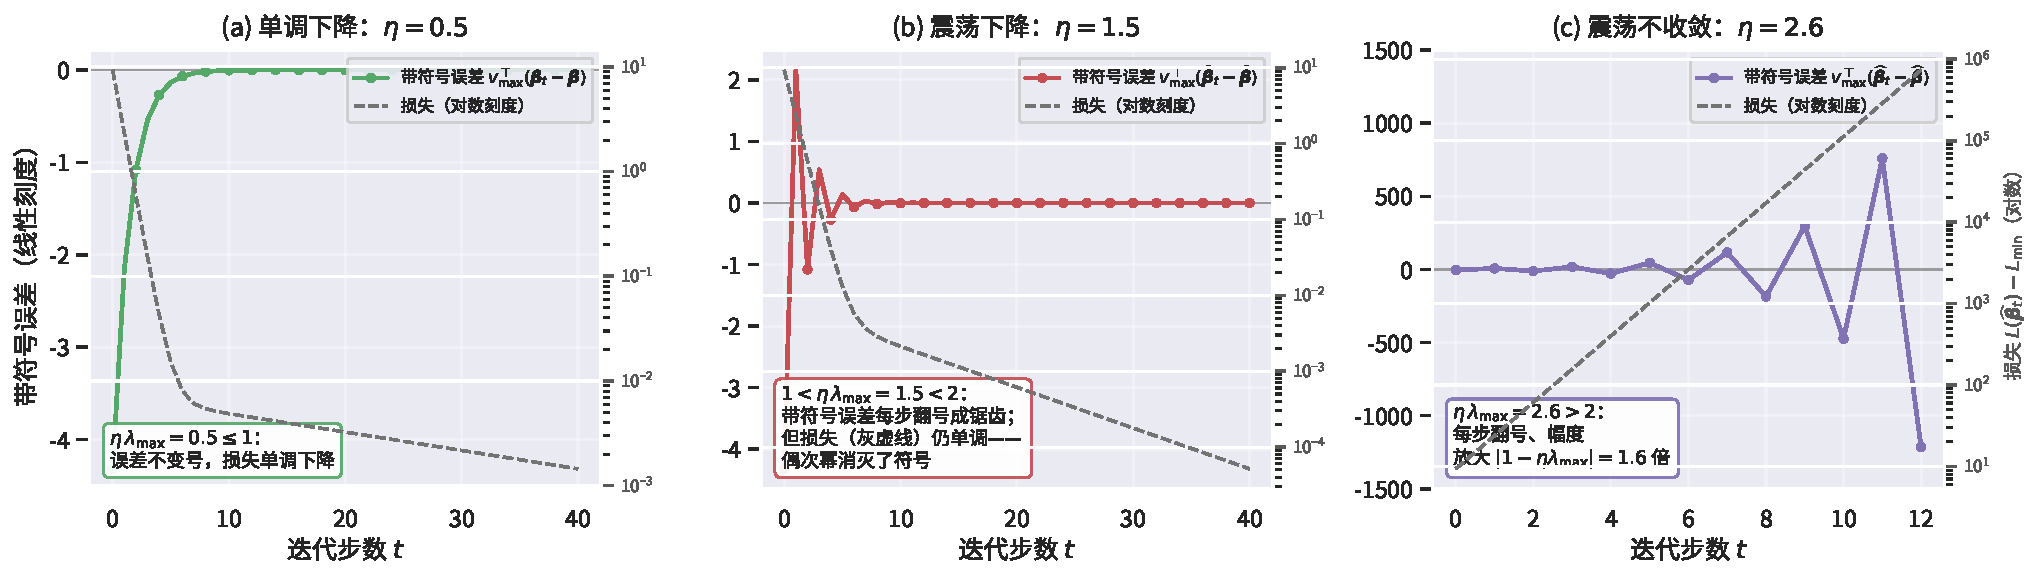
\includegraphics[width=\linewidth]{figures/ch4_loss.pdf}
  \caption{带符号误差（彩色实线，左轴，线性刻度）与损失（灰虚线，右轴，对数刻度）随迭代步数 $t$ 的三档形态（同一二次问题、同一初值、仅改变 $\eta$）：(a) 单调下降——$\eta\lambda_{\max} \le 1$，最大特征方向误差不变号，损失单调；(b) 震荡下降——$1 < \eta\lambda_{\max} < 2$，带符号误差每步翻号成锯齿，但损失因偶次幂仍单调下滑；(c) 震荡不收敛——$\eta\lambda_{\max} > 2$，误差每步翻号、幅度以 $|1-\eta\lambda_{\max}|$ 倍放大，损失爆炸。}
  \label{fig:ch4-loss}
\end{figure}

两个实践推论，都是「为什么学线性回归」的答案碎片：

\begin{itemize}
  \item \textbf{条件数统治一切。}$\kappa \approx 1$（特征方向长短一致）时 $\rho^\star \approx 0$，几步收敛；$\kappa \gg 1$（第 \ref{sec:hd-break} 节的病态）时 $\rho^\star \approx 1 - 2/\kappa$，收敛以 $O(\kappa \log(1/\varepsilon))$ 步计——\textit{与特征缩放强相关的工程经验「先标准化特征」}，在这里是半个定理：标准化把 $\X^\top\X$ 的对角元归一，\textbf{消除了条件数中由量纲差异贡献的部分}——但由\textbf{相关结构}（共线）造成的特征值分散完全不受影响，$\kappa$ 仍可以很大。
  \item \textbf{预处理 = 坐标变换下的 GD。}对 $\X^\top\X$ 做谱分解后做白化，等价于在更好的坐标系里跑梯度下降；共轭梯度法（CG）则可视为「每步自动选步长与方向的 GD」，$d$ 步内\textbf{精确}到达 $\bhat$（二次函数的有限终止性）。从 GD 到 CG 到直接求逆，是一个谱系，两端是「迭代 $t$ 步」与「闭式一步」，中间全是同一几何的插值。
\end{itemize}

\begin{figure}[htbp]
  \centering
  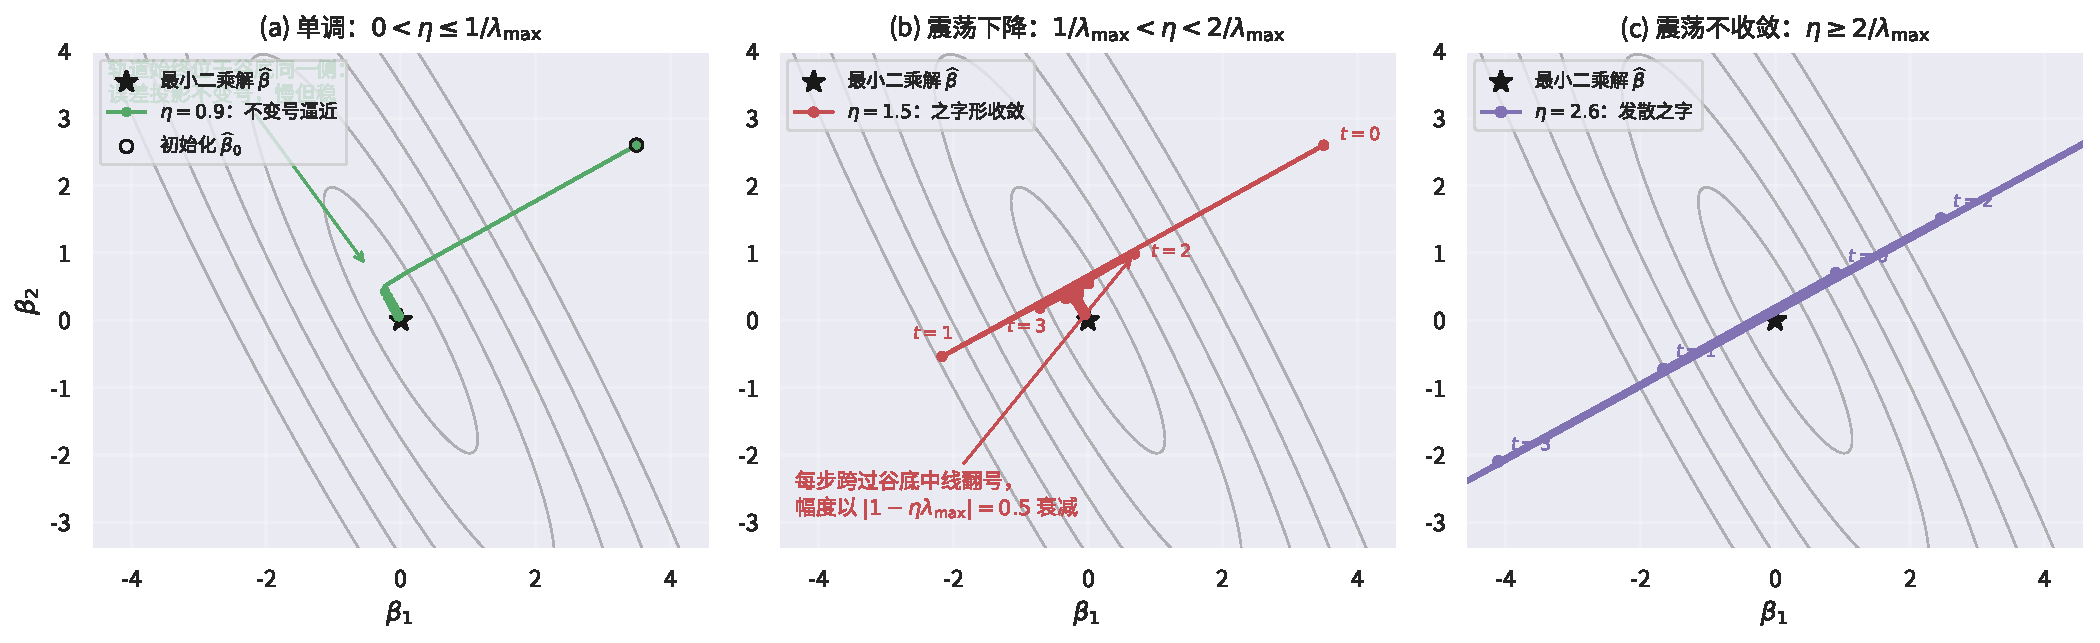
\includegraphics[width=\linewidth]{figures/ch4_gd.pdf}
  \caption{梯度下降在二次损失（条件数 $\kappa=25$ 的椭圆谷）上的三条轨道，与步长三档一一对应：(a) $\eta=0.9 \le 1/\lambda_{\max}$：轨道不跨谷底中线、不变号逼近，但沿「瘦」方向缓慢爬行；(b) $1/\lambda_{\max}<\eta=1.5<2/\lambda_{\max}$：轨道每步跨过谷底翻号，之字形幅度以 $|1-\eta\lambda_{\max}|=0.5$ 衰减——震荡下降；(c) $\eta=2.6>2/\lambda_{\max}$：每步翻号、幅度放大 $1.6$ 倍，数步内飞出视野。}
  \label{fig:ch4-gd}
\end{figure}

\subsection{与闭式解的对照表}

\begin{center}
\begin{tabular}{@{}lll@{}}
\toprule
 & 闭式解 $\bhat = (\X^\top\X)^{-1}\X^\top\y$ & 梯度下降 \eqref{eq:gd} \\
\midrule
性质 & 一步到位（解 $d\times d$ 系统） & 逐步逼近，$t$ 步后误差 $\propto \rho^t$ \\
代价（列满秩） & $O(nd^2 + d^3)$，须形成 $\X^\top\X$ & 每步 $O(nd)$ 矩阵向量乘，内存友好 \\
适用区域 & $n \gg d$ 的经典区间 & 任意 $n, d$（配合正则化/早期停止） \\
病态 $\kappa \gg 1$ & 数值不稳定（条件数平方） & 收敛极慢（同样的 $\kappa$，不同的病法） \\
与 $\bhat$ 的关系 & 就是它 & 不动点即 $\bhat$；$\widehat{\bbeta}_t$ 有精确解 \eqref{eq:gd-exact} \\
\bottomrule
\end{tabular}
\end{center}

\begin{keybox}[本章要点]
\begin{itemize}
  \item 梯度下降迭代 $\widehat{\bbeta}_{t+1} = \widehat{\bbeta}_t - \eta\,\X^\top(\X\widehat{\bbeta}_t - \y)$ 的不动点条件 $\nabla L = \zero$ 就是正规方程，唯一不动点即闭式解 $\bhat$——优化视角与代数视角终点相同；
  \item 联立两式得精确解 $\widehat{\bbeta}_t = \bhat + (\bm{I} - \eta\X^\top\X)^t(\widehat{\bbeta}_0 - \bhat)$：误差每步左乘 $\bm{I} - \eta\X^\top\X$，特征值 $1 - \eta\lambda_j$ 决定各方向衰减；
  \item 收敛当且仅当 $0 < \eta < 2/\lambda_{\max}$；最优 $\eta^\star = 2/(\lambda_{\min} + \lambda_{\max})$，渐近率 $(\kappa - 1)/(\kappa + 1)$——「标准化特征」消除量纲导致的病态（相关结构导致的病态它无能为力）；
  \item GD 的几何级数形式说明它在用 $t$ 次多项式逼近 $(\X^\top\X)^{-1}$：闭式解直给逆，迭代解按揭逆；共轭梯度是谱系的中点。
\end{itemize}
\end{keybox}

\begin{exercise}\label{ex:gd-rate}
由 \eqref{eq:gd-exact} 推导：若 $\widehat{\bbeta}_0 = \zero$ 且 $\eta = \eta^\star$，则 $\norm{\widehat{\bbeta}_t - \bhat} \le \big(\frac{\kappa-1}{\kappa+1}\big)^t \norm{\bhat}$；并由此给出达到 $\norm{\widehat{\bbeta}_t - \bhat} \le \varepsilon$ 所需步数的 $O(\cdot)$ 表达式。
\end{exercise}

\begin{exercise}\label{ex:neumann}
验证恒等式 $\eta\sum_{k=0}^{t-1}(\bm{I} - \eta\X^\top\X)^k \X^\top\y = \big[\bm{I} - (\bm{I} - \eta\X^\top\X)^t\big]\bhat$（提示：两边同乘 $\X^\top\X$ 或用 Neumann 级数），说明它正是 \eqref{eq:gd-exact-zero} 的左乘形式。
\end{exercise}

\clearpage
% 第 5 章
\section{另一个不动点：当 $d > n$ 时梯度下降去向何处}\label{sec:gd-underdet}

第 \ref{sec:gd} 章的精确解 \eqref{eq:gd-exact} 有一个隐藏前提：$\X^\top\X$ 可逆。本章转向相反的\textbf{欠定}（underdetermined）情形 $d > n$：方程个数少于未知数，$\X^\top\X \in \R^{d \times d}$ 必奇异（秩 $\le n < d$），闭式解 \eqref{eq:ols-closed} 不复存在，第 \ref{sec:gd} 章的衰减矩阵 $\bm{I} - \eta\X^\top\X$ 有 $d - n$ 个特征值恒等于 $1$——误差在某些方向上\textbf{永不衰减}。然而正是在这里，gradient descent 给出了一个深刻的结果：\textbf{迭代依然收敛，只是收敛到一个由初值选定的特殊解；从 $\widehat{\bbeta}_0 = \zero$ 出发，它收敛到最小范数解}
\[
  \widehat{\bbeta}' = \X^\top (\X \X^\top)^{-1} \y .
\]

\subsection{设定：$d > n$，解已成流形}\label{sec:underdet-setup}

设 $\X \in \R^{n \times d}$ \textbf{行满秩}（$\rank(\X) = n$，即 $n$ 行线性无关；连续分布的随机数据几乎必然如此），则 $\X\X^\top \in \R^{n \times n}$ 对称正定、可逆。此时：

\begin{itemize}
  \item 方程组 $\X \bbeta = \y$ \textbf{相容}（$\y$ 必在列空间内），且解\textbf{不唯一}：通解为
  \[
    \big\{ \bbeta : \X \bbeta = \y \big\} = \widehat{\bbeta}' + \mathcal{N}(\X),
    \qquad
    \mathcal{N}(\X) = \{ \bm{w} \in \R^d : \X \bm{w} = \zero \},
  \]
  一个 $d - n$ 维的仿射子空间（解流形）——每个点都是一个插值解；
  \item 损失 $L(\bbeta) = \frac{1}{2}\norm{\y - \X\bbeta}^2$ 在该流形上恒为零，即全局最小值为 $0$ 且\textbf{在一个流形上取到}；
  \item $\X^\top\X$ 有 $d - n$ 个零特征值，$(\X^\top\X)^{-1}$ 无定义——第 \ref{sec:gd} 章的全部公式在此处失效。
\end{itemize}

\subsection{一个新的不动点及其两个验证}

\subsubsection*{验证 1：精确插值}
直接代入：
\begin{equation}\label{eq:interp}
  \X \, \widehat{\bbeta}' = \X \X^\top (\X \X^\top)^{-1} \y = \y .
\end{equation}
即 $y = \X \widehat{\bbeta}'$：训练误差精确为零——\textbf{插值}（interpolation）。这正是 $d = n$ 时「残差为零」现象（第 \ref{sec:hd-break} 节）在 $d > n$ 时的延续：模型容量过剩，拟合变成了记忆。

\subsubsection*{验证 2：一阶平衡点}
梯度为
\begin{equation}\label{eq:grad-at-p}
  \nabla L(\widehat{\bbeta}') = \X^\top \big( \X \widehat{\bbeta}' - \y \big) = \X^\top ( \y - \y ) = \zero .
\end{equation}
即 $\widehat{\bbeta}'$ 是 least-square 损失的一个\textbf{一阶平衡点}（驻点）；由 $L$ 凸且 $L(\widehat{\bbeta}') = 0 = \min L$，它其实还是全局最小点。于是它也是 GD 迭代 \eqref{eq:gd} 的不动点：$\widehat{\bbeta}' - \eta\, \nabla L(\widehat{\bbeta}') = \widehat{\bbeta}'$ 对\textbf{任意} $\eta$ 成立。事实上由 \eqref{eq:grad-at-p} 可见：\textbf{整个解流形 $\widehat{\bbeta}' + \mathcal{N}(\X)$ 上的每一点都是不动点}——这不是一个孤立的平衡点，而是一整个平衡点集合。

\subsection[最小范数性：解流形上离原点最近的点]{最小范数性：$\widehat{\bbeta}'$ 是解流形上离原点最近的点}\label{sec:minnorm}

\begin{theorem}[最小范数解]\label{thm:minnorm}
在解流形 $\{ \bbeta : \X \bbeta = \y \}$ 上，$\widehat{\bbeta}' = \X^\top(\X\X^\top)^{-1}\y$ 是唯一的 Euclidean 范数最小点。
\end{theorem}
\begin{proof}
任取解 $\bbeta$，写 $\bbeta = \widehat{\bbeta}' + \bm{w}$，其中 $\X\bm{w} = \zero$（两解之差在零空间内）。关键观察：$\widehat{\bbeta}' \perp \mathcal{N}(\X)$，因为
\[
  \langle \widehat{\bbeta}',\ \bm{w} \rangle = \y^\top (\X\X^\top)^{-1} \X\, \bm{w} = 0 .
\]
于是由勾股定理
\[
  \norm{\bbeta}^2 = \norm{\widehat{\bbeta}'}^2 + \norm{\bm{w}}^2 \;\ge\; \norm{\widehat{\bbeta}'}^2,
\]
等号当且仅当 $\bm{w} = \zero$。$\widehat{\bbeta}'$ 正是解流形在 row$(\X)$（$\X^\top$ 的列空间）上的那个点。
\end{proof}

\subsection{稳定性：行空间收缩，零空间中性}\label{sec:stability}

不动点集合那么大，迭代到底收不收敛、收敛到哪？把第 \ref{sec:gd} 章的稳定性分析搬过来，只换特征谱。GD 映射 $\bm{G}(\bbeta) = \bbeta - \eta \nabla L(\bbeta)$ 的线性化（它本身就是线性的）为
\[
  \bm{G}(\bbeta) - \bm{G}(\bbeta_0) = (\bm{I} - \eta \X^\top \X)(\bbeta - \bbeta_0).
\]
$\X^\top\X$ 的特征值：$n$ 个正特征值 $\lambda_1 \ge \dots \ge \lambda_n > 0$（与 $\X\X^\top$ 的非零特征值完全相同），外加 $d - n$ 个 $0$。于是 $\bm{I} - \eta\X^\top\X$ 的特征值为
\[
  \underbrace{1 - \eta \lambda_j}_{n \text{ 个}},\ j = 1..n;
  \qquad
  \underbrace{1}_{d - n \text{ 个}}.
\]
\begin{itemize}
  \item \textbf{行空间方向}（$d - n$ 个零特征值对应方向的正交补）：当 $0 < \eta < \dfrac{2}{\lambda_{\max}(\X\X^\top)}$ 时 $|1 - \eta\lambda_j| < 1$——\textbf{收缩}，与 $n \gg d$ 情形完全相同的指数衰减；
  \item \textbf{零空间方向}：因子恒为 $1$——\textbf{中性}：初始误差中的 $\mathcal{N}(\X)$ 分量\textbf{原样保留，永不衰减}。
\end{itemize}

结论分层说清楚：
\begin{enumerate}[label=(\arabic*)]
  \item 解流形 $\widehat{\bbeta}' + \mathcal{N}(\X)$ 上的\textbf{每一个点都是 Lyapunov 稳定}的：横向（行空间）扰动被指数压回流形附近，切向（零空间）扰动既不放大也不消失，迭代始终停留在扰动点的有界邻域内；
  \item 作为\textbf{孤立的点}，流形上的每个平衡点都不是渐近稳定的（切向的小扰动不会回来）——稳定的是\textbf{流形本身}：它是横向吸引的（normally attracting）；
  \item \textbf{初值决定落点}：由于零空间分量守恒，$\widehat{\bbeta}_0$ 的零空间分量被一路携带到极限——
  \[
    \lim_{t \to \infty} \widehat{\bbeta}_t = \widehat{\bbeta}' + \underbrace{\bm{P}_{\mathcal{N}(\X)}\, \widehat{\bbeta}_0}_{\text{零空间分量}} ,
  \]
  其中 $\bm{P}_{\mathcal{N}(\X)}$ 是到零空间的正交投影。
\end{enumerate}

\subsection{精确解（续）：GD 从零点出发 = 隐式最小范数正则化}\label{sec:implicit}

取最常见的初值 $\widehat{\bbeta}_0 = \zero$：零空间分量为零，于是迭代的\textbf{全程都待在 row$(\X)$ 里}（归纳可见 $\widehat{\bbeta}_t = \X^\top \bm{u}_t$ 对某 $\bm{u}_t$ 成立，因为梯度 $\X^\top(\cdot)$ 总把向量拉回行空间）。行空间里只有一个插值点——就是 $\widehat{\bbeta}'$。于是：

\begin{theorem}[欠定情形的 GD 精确解]\label{thm:gd-exact-underdet}
设 $\X$ 行满秩，$0 < \eta < 2/\lambda_{\max}(\X\X^\top)$，$\widehat{\bbeta}_0 = \zero$。则
\begin{equation}\label{eq:gd-exact-underdet}
  \boxed{\;\widehat{\bbeta}_t = \Big[ \bm{I} - \big( \bm{I} - \eta\, \X^\top \X \big)^{t} \Big]\, \X^\top (\X \X^\top)^{-1} \y
       = \Big[ \bm{I} - \big( \bm{I} - \eta\, \X^\top \X \big)^{t} \Big]\, \widehat{\bbeta}'\;}
\end{equation}
且 $\widehat{\bbeta}_t \to \widehat{\bbeta}'$（最小范数插值解），收敛率由 $\X\X^\top$ 的条件数决定：$\norm{\widehat{\bbeta}_t - \widehat{\bbeta}'} = O\big( \big(\frac{\kappa - 1}{\kappa + 1}\big)^t \big)$（在最优步长下）。
\end{theorem}
\begin{proof}
用恒等式 $\X^\top (\bm{I} - \eta \X\X^\top) = (\bm{I} - \eta \X^\top\X) \X^\top$（两边都等于 $\X^\top - \eta \X^\top \X \X^\top$）对 \eqref{eq:gd} 递推，得 $\widehat{\bbeta}_t = \X^\top \big[ \eta \sum_{k=0}^{t-1} (\bm{I} - \eta\X\X^\top)^k \big] \y$。括号内是 $\R^{n \times n}$ 上的几何级数，$\eta < 2/\lambda_{\max}$ 保证其谱半径小于 $1$（全部特征严格收缩），于是 $\eta \sum_{k<t}(\bm{I} - \eta\X\X^\top)^k = \big[ \bm{I} - (\bm{I} - \eta\X\X^\top)^t \big](\X\X^\top)^{-1}$，代回并再次使用上述恒等式即得 \eqref{eq:gd-exact-underdet}。极限由 $(\bm{I} - \eta\X\X^\top)^t \to \zero$ 给出；收敛率照搬推论 \ref{thm:gd-opt}，只是把 $\X^\top\X$ 的谱换成 $\X\X^\top$ 的谱（非零特征值相同）。
\end{proof}

把 \eqref{eq:gd-exact-underdet} 与 \eqref{eq:gd-exact-zero} 并排看，结构完全一致——\textbf{唯一的差别是「目标点」从 $\bhat = (\X^\top\X)^{-1}\X^\top\y$ 换成了 $\widehat{\bbeta}' = \X^\top(\X\X^\top)^{-1}\y$}。形式上的对称绝非巧合，下一节给出统摄两者的对象。

\begin{remark}[隐式正则化]
定理 \ref{thm:gd-exact-underdet} 是现代「隐式正则化 / 隐式偏差」（implicit regularization / implicit bias）理论的原型：\textbf{没有任何显式惩罚项，单纯从零点做梯度下降，就自动选出了所有插值解中范数最小、因而往往最泛化的那一个}。过参数化神经网络在训练中「不爆记忆、反而泛化」的现象，其最干净的数学化身就是这个线性版本。
\end{remark}

\begin{figure}[htbp]
  \centering
  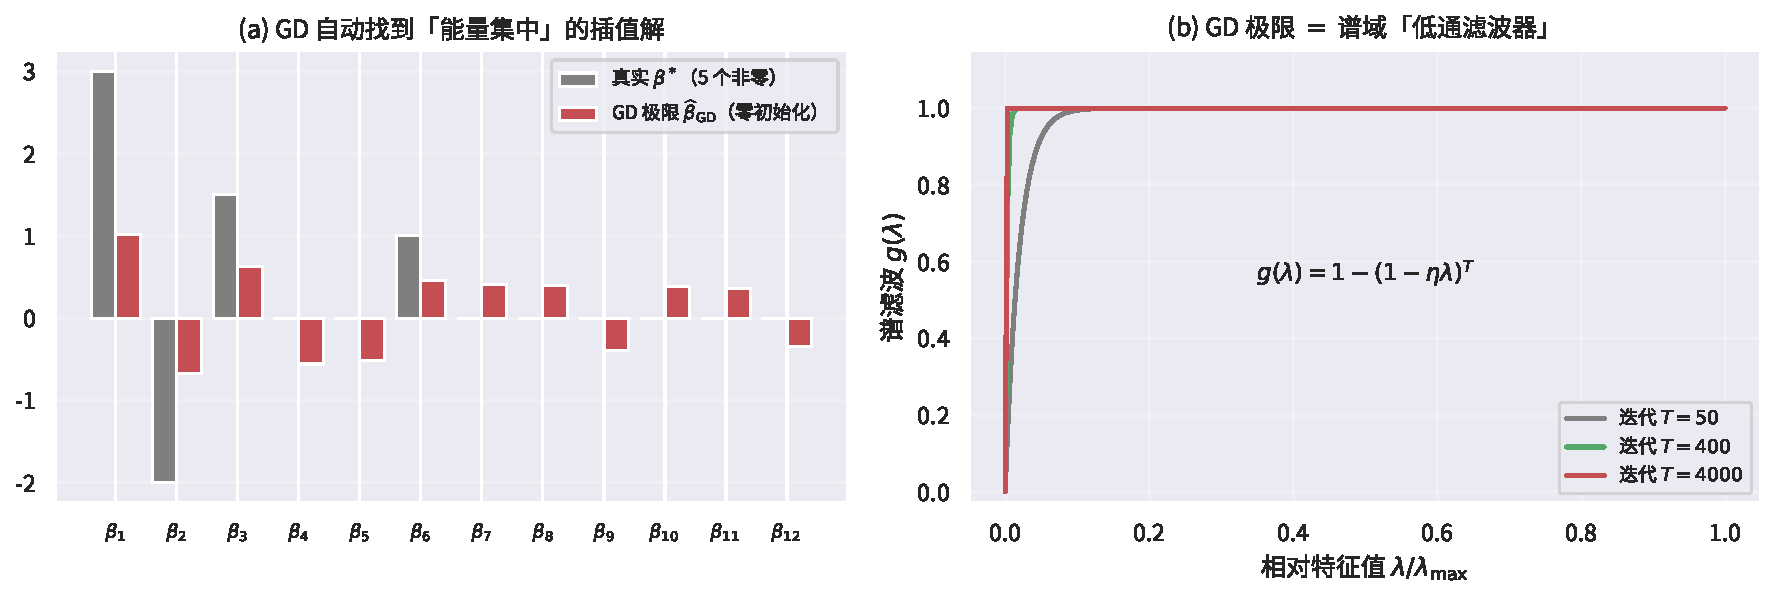
\includegraphics[width=\linewidth]{figures/ch5_implicit.pdf}
  \caption{隐式正则化的两个面孔（$d=100>n=30$，无噪声插值）：(a) 零初始化 GD 的极限（红）在真实信号方向（灰，5 个非零系数）上恢复能量、在噪声方向自动收缩；(b) 谱滤波解释——$t$ 步 GD 在特征方向 $\lambda$ 上施加因子 $g(\lambda)=1-(1-\eta\lambda)^t$，大特征方向先收敛、小特征方向后收敛，等效于一个「低通滤波器」。}
  \label{fig:ch5-implicit}
\end{figure}

\subsection{与伪逆解的比较：一个对象，几张面孔}\label{sec:pseudo-compare}

现在回答本章的比较问题。Moore--Penrose 伪逆 $\X^+$ 由 SVD 统一定义：若 $\X = \bm{U} \bm{\Sigma} \bm{V}^\top$（$\bm{\Sigma}$ 对角、元为奇异值 $s_j > 0$），则
\[
  \X^+ = \bm{V} \bm{\Sigma}^{+} \bm{U}^\top, \qquad
  \bm{\Sigma}^{+} \text{ 把每个 } s_j \text{ 换成 } 1/s_j \ (\text{零保持不变}).
\]
它给出\textbf{任意} $\X$ 的\textbf{最小范数最小二乘解} $\X^+\y$。两个秩情形分别退化为两个熟悉的公式：

\begin{itemize}
  \item \textbf{列满秩}（$n \gg d$）：$\X^+ = (\X^\top\X)^{-1}\X^\top$——第 \ref{sec:hd-closed} 节的 OLS 闭式解；
  \item \textbf{行满秩}（$d > n$）：$\X^+ = \X^\top(\X\X^\top)^{-1}$——\textbf{正是本节的 $\widehat{\bbeta}'$}。（代入 SVD 即可验证：$\X\X^\top = \bm{U}\bm{\Sigma}\bm{\Sigma}^\top\bm{U}^\top$，逆为 $\bm{U}(\bm{\Sigma}\bm{\Sigma}^\top)^{-1}\bm{U}^\top$，左乘 $\X^\top = \bm{V}\bm{\Sigma}^\top\bm{U}^\top$ 得 $\bm{V}\bm{\Sigma}^+\bm{U}^\top$。）
\end{itemize}

所以：\textbf{在 $d > n$ 行满秩时，$\widehat{\bbeta}'$ 就是伪逆解}——不是「另一个解」，而是同一对象在欠定 regime 的面孔。下表把全文出现的所有「同一个点」的到达方式收拢：

\begin{center}
\resizebox{\linewidth}{!}{%
\begin{tabular}{@{}llll@{}}
\toprule
对象 & 公式 & 适用 & 到达方式 \\
\midrule
OLS 闭式解 & $(\X^\top\X)^{-1}\X^\top\y$ & $n \gg d$ 列满秩 & 直接解正规方程 \\
\textbf{本章 $\widehat{\bbeta}'$} & $\X^\top(\X\X^\top)^{-1}\y$ & $d > n$ 行满秩 & 直接解插值方程 \\
伪逆解 $\X^+\y$ & SVD 定义 & 任意秩 & 统一定义（上两者的母对象） \\
GD，$\widehat{\bbeta}_0 = \zero$ & $\lim_t \widehat{\bbeta}_t$ & 任意秩 & 隐式收敛到 $\X^+\y$（本两章精确解） \\
ridge，$\lambda \to 0^+$ & $\lim_{\lambda \to 0^+}(\X^\top\X + \lambda\bm{I})^{-1}\X^\top\y$ & 任意秩 & 同 $\X^+\y$（恒等式取极限，见练习） \\
\bottomrule
\end{tabular}}
\end{center}

两点比较结论值得单独记住：

\begin{enumerate}[label=(\arabic*)]
  \item \textbf{代数上}：$\widehat{\bbeta}' = \X^+\y$（行满秩时）——它与伪逆解\textbf{完全相同}，包括那条「最小范数」性质：伪逆的全部定义性质中，$\X^+\y \perp \mathcal{N}(\X)$ 这一条在欠定情形正是定理 \ref{thm:minnorm} 的内容。
  \item \textbf{动力学上}：伪逆是「静态」的（SVD 一刀切出答案），GD 是「动态」的（多项式一步步逼近）：\eqref{eq:gd-exact-underdet} 显示 GD 的 $t$ 步解 $= \big[\bm{I} - (\bm{I} - \eta\X^\top\X)^t\big]\X^+\y$，括号内是作用在伪逆解上的收缩多项式。换一个初值，GD 还会走到\textbf{别的}插值点（带上初值的零空间分量）——\textit{GD 族抵达的是整个解流形，伪逆（以及零点初值）选中的是流形上离原点最近的那一点}。
\end{enumerate}

\begin{keybox}[本章要点]
\begin{itemize}
  \item $d > n$ 行满秩时 $\widehat{\bbeta}' = \X^\top(\X\X^\top)^{-1}\y$ 满足 (i) 精确插值 $\X\widehat{\bbeta}' = \y$、(ii) $\nabla L(\widehat{\bbeta}') = \zero$（一阶平衡点），且是解流形上\textbf{唯一的最小范数}点；
  \item 整个解流形 $\widehat{\bbeta}' + \mathcal{N}(\X)$ 都是 GD 的不动点：行空间方向（$0 < \eta < 2/\lambda_{\max}(\X\X^\top)$ 时）指数收缩，零空间方向中性——流形横向吸引、点仅 Lyapunov 稳定，落点由初值的零空间分量决定；
  \item 精确解 $\widehat{\bbeta}_t = [\bm{I} - (\bm{I} - \eta\X^\top\X)^t]\widehat{\bbeta}'$：与 $n \gg d$ 情形结构同构，目标点由 $\bhat$ 换成 $\widehat{\bbeta}'$；$\widehat{\bbeta}_0 = \zero$ 时 GD \textbf{隐式}收敛到最小范数解——隐式正则化的线性原型；
  \item 与伪逆的关系：行满秩时 $\widehat{\bbeta}' = \X^+\y$ 恒等；伪逆、两个闭式公式、GD 零点极限、ridge 零极限是\textbf{同一个最小范数最小二乘解}的五张面孔。
\end{itemize}
\end{keybox}

\begin{exercise}\label{ex:ridge-dual}
证明恒等式 $(\X^\top\X + \lambda\bm{I})^{-1}\X^\top = \X^\top(\X\X^\top + \lambda\bm{I})^{-1}$（两边同乘 $(\X^\top\X + \lambda\bm{I})$ 并整理），并由此说明 ridge 解在 $\lambda \to 0^+$ 时收敛到 $\X^+\y$（无需满秩假设）。
\end{exercise}

\begin{exercise}\label{ex:gd-limit-anyinit}
设 $d > n$、$\X$ 行满秩。证明：对任意初值 $\widehat{\bbeta}_0$，GD 的极限为 $\widehat{\bbeta}' + \bm{P}_{\mathcal{N}(\X)} \widehat{\bbeta}_0$，其中 $\bm{P}_{\mathcal{N}(\X)} = \bm{I} - \X^+\X$ 是到零空间的正交投影；并解释为何这一结论与定理 \ref{thm:gd-exact-underdet} 一致。
\end{exercise}

\begin{exercise}\label{ex:spectrum}
对比两个 regime 的「有效维数」：$n \gg d$ 时 GD 误差衰减由 $\X^\top\X$ 的 $d$ 个特征值决定；$d > n$ 时由 $\X\X^\top$ 的 $n$ 个特征值决定。证明两矩阵的非零特征值完全相同（提示：若 $\X^\top\X \bm{v} = \lambda \bm{v}$，考察 $\X \bm{v}$），并解释这一谱同一性为何使两章的收敛率公式可以互换。
\end{exercise}

\clearpage
% 第 7 章
\section{从估计到推断：协方差、精度矩阵与条件独立}\label{sec:ggm}

第 \ref{sec:onedim} 章在一维世界里弄清了「相关 $\neq$ 因果」。本章把问题升格到联合层面：把 $(y, \x)$ 当作一个 $(d{+}1)$ 维随机向量，问\textbf{协方差矩阵与它的逆（精度矩阵）}如何编码 $y$ 与 $\X$ 之间的相关、条件独立与（在图假设下的）因果结构；再回答实践问题：$d$ 很大、$n$ 很小时如何估计（lasso、elastic net、CLIME、graphical lasso），以及如何把「点估计」升级为「推断」（debiased lasso）——即\textbf{from estimate to inference}。

\subsection{协方差与精度矩阵：相关的两种编码}\label{sec:cov-prec}

设 $(y, \x)$ 联合高斯，均值不妨为零，记
\[
  \bm{\Sigma} = \Cov\begin{pmatrix} y \\ \x \end{pmatrix} \succ \zero,
  \qquad
  \bm{\Theta} = \bm{\Sigma}^{-1} \ \text{(精度矩阵, precision matrix)}.
\]
两个矩阵编码两种不同的「相关」：

\begin{itemize}
  \item \textbf{协方差 $\Sigma_{ij} \neq 0$}：边际相关（marginal correlation）。它会\textit{传导}：即使 $y \perp x_j$ 在控制其余变量后成立（无直接联系），$x_j$ 仍可与 $y$ 边际相关——只要存在一条经其他变量的间接路径（第 \ref{sec:1d-causality} 节共同原因结构的多变量版本）。
  \item \textbf{精度矩阵元 $\Theta_{ij} = 0$}：\textbf{条件独立}。高斯情形有精确恒等式
  \begin{equation}\label{eq:ci-prec}
    \Theta_{ij} = 0
    \quad\Longleftrightarrow\quad
    i \perp j \mid \text{其余所有变量},
    \qquad
    \rho_{ij \cdot V \setminus \{i,j\}} = -\frac{\Theta_{ij}}{\sqrt{\Theta_{ii}\,\Theta_{jj}}} \ \text{(偏相关系数)} .
  \end{equation}
  即：\textit{偏相关为零 $\Leftrightarrow$ 在给定其他一切变量的条件下两者独立}。证明只需分块求逆（练习 \ref{ex:block-inv}）。
\end{itemize}

\eqref{eq:ci-prec} 是本章的枢纽：\textbf{精度矩阵的零模式是一张「条件独立图」的邻接矩阵}——高斯图模型（Gaussian graphical model）\cite{lauritzen1996}。相关沿图\textit{流动}（间接路径也产生相关），条件独立只在\textit{无边}时成立；这张图就是 Wright 路径图（第 \ref{sec:1d-causality} 节）的高斯化身。

\subsection{回归系数是精度矩阵的元素}\label{sec:beta-theta}

现在把线性回归接上这张图。对联合高斯做分块：$\bm{\Theta} = \begin{pmatrix} \Theta_{yy} & \bm{\Theta}_{yX} \\ \bm{\Theta}_{Xy} & \bm{\Theta}_{XX} \end{pmatrix}$（标量 $\Theta_{yy} > 0$，$\bm{\Theta}_{Xy} \in \R^d$）。由分块求逆（练习 \ref{ex:block-inv}），给定 $\X$ 时 $y$ 的条件分布为
\begin{equation}\label{eq:conditional}
  y \mid \X \sim \mathcal{N}\Big( -\tfrac{1}{\Theta_{yy}}\, \bm{\Theta}_{yX}^\top \x,\ \tfrac{1}{\Theta_{yy}} \Big).
\end{equation}
与回归模型 $y = \x^\top \bbeta + \varepsilon$ 对照，得到一组应当刻在石头上的恒等式：
\begin{equation}\label{eq:beta-theta}
  \boxed{\;\bbeta = -\frac{\bm{\Theta}_{Xy}}{\Theta_{yy}}, \qquad \Var(\varepsilon) = \frac{1}{\Theta_{yy}}\;}
\end{equation}

\begin{keybox}[回归 = 探查图结构]
\eqref{eq:beta-theta} 说：\textbf{回归系数（及其符号、显著性）是精度矩阵元素的比值}。特别地，
\[
  \beta_j = 0
  \quad\Longleftrightarrow\quad
  \Theta_{Xy,j} = 0
  \quad\Longleftrightarrow\quad
  y \perp x_j \mid \x_{-j}
  \ \text{（在控制其余特征后，$y$ 与 $x_j$ 条件独立）}.
\]
\end{keybox}

这句话把一个统计问题翻译成两个问题：
\begin{enumerate}[label=(\arabic*)]
  \item \textbf{相关}（第 \ref{sec:onedim} 章）：$y$ 与 $x_j$ 是否边际相关？——看 $\Sigma$，一个 $t$ 检验的事；
  \item \textbf{条件独立}：控制其余变量后，$y$ 与 $x_j$ 是否仍有「直接」联系？——看 $\Theta$ 的零模式，即\textbf{偏相关}是否为零。
\end{enumerate}
两者的差距正是「$x_j$ 与 $y$ 的相关完全由第三个变量解释」这类现象（混杂、中介）的矩阵语言。注意 $\beta_j = 0$ 给出的是\textbf{图论意义上的「无直接边」}，而不是因果断言——除非图本身已被外部知识（第 \ref{sec:1d-causality} 节）或下文的条件独立检验约束到可识别。

\subsection{条件独立检验与因果：从相关到图}\label{sec:ci-causal}

\eqref{eq:ci-prec} 提供了\textbf{可检验的约束}：高斯图上每条缺失的边都对应一个「偏相关为零」的统计假设
\begin{equation}\label{eq:ci-test}
  H_0^{(ij)}:\ \rho_{ij\cdot V\setminus\{i,j\}} = 0
  \quad(\Longleftrightarrow\ \Theta_{ij} = 0),
\end{equation}
可用 Fisher 的 $z$ 变换在小维情形直接检验；在高维情形，逐个检验不再可行，但约束的逻辑不变。PC 算法（Spirtes, Glymour \& Scheines）展示了这套约束如何变成因果发现\cite{spirtes2000}：

\begin{enumerate}[label=(\alph*)]
  \item \textbf{删边}：对每对变量搜索条件集 $S$，一旦检验出 $i \perp j \mid S$ 就在 $i,j$ 间删去无向边——共同原因与间接路径在这条检验现形（这正是 Reichenbach 原理 \cite{reichenbach1956} 的可操作版本）；
  \item \textbf{定向}：对 $i - k - j$ 且 $i, j$ 不相邻的结构（v-结构），在 Markov + faithfulness 假设下可定向 $i \to k \leftarrow j$——\textbf{数据本身对一部分箭头给出了方向}；
  \item \textbf{传播}：Meek 规则把方向沿图继续传播。
\end{enumerate}

与第 \ref{sec:1d-causality} 节呼应：相关系数本身永不给方向，但\textbf{一组条件独立检验}能在「图 faithful 于分布」的额外假设下恢复出部分 DAG；因果结论的合法性仍然来自假设清单，而不是来自数据本身——只是现在假设可以被逐一检验、逐一反驳。

\subsection{稀疏性：为什么「大多数系数是零」是可计算的假设}\label{sec:sparsity}

前两节给出了图模型的语言：$d$ 个变量之间至多有 $\binom{d}{2}$ 条边、$d^2$ 个精度矩阵元素要估计。当 $d > n$ 时这是不可能完成的任务——除非我们愿意相信一件很具体的事：\textbf{真实的图是稀疏的}，大多数 $\Theta_{ij} = 0$。本节解释为什么这个假设不仅合理，而且是「可计算的」。

\textbf{稀疏性是可证伪的假设，不是祈祷。}「大多数系数为零」意味着图有 $s \ll d^2$ 条边；若真实边数 $s$ 满足 $s \log d \ll n$，则有一类方法（下一节）能以高概率\textbf{恰好}恢复图的结构。反过来，若数据真是稠密的，稀疏方法的失败会以「交叉验证选不出稳定结构」的形式诚实地暴露——这与第 \ref{sec:1d-causality} 章「先拟合、审计假设」的精神一致：稀疏假设可以且应当被审计。

\textbf{稀疏性从何而来？}三个独立的来源。(1) \textbf{科学的}：基因调控网络中每个基因只被少数转录因子调控，社交网络每人只有若干紧密联系人——「每行非零元有界」是许多领域的先验知识，对应数学上的 $s = O(d)$ 条边。(2) \textbf{统计的}：在适当设计下，稀疏模型的有效自由度 $\ll d$（见下），样本复杂度由\textbf{非零元个数}而非维数决定——这正是「高维统计」一词的本义：$d$ 可以大于 $n$，只要真实参数的支撑集小于 $n$。(3) \textbf{计算的}：稀疏性把一个 $d^2$ 维的连续优化问题变成「找哪些坐标非零 + 估它们的值」，而后者有明确的算法与误差界。

\textbf{稀疏性的三个面孔，一句话一个。}
\begin{enumerate}[label=(\arabic*)]
  \item \textbf{组合面孔}：模型选择——在 $2^d$ 个子集中找正确的一个。NP-hard 的一般问题在稀疏假设下可解（$s$ 小使搜索空间塌缩）。
  \item \textbf{几何面孔}：$\ell_0$ 球 $\{\bbeta : \norm{\bbeta}_0 \le s\}$ 非凸，$\ell_1$ 是它的\textbf{凸松弛}（严格的包络关系是 $\norm{\bbeta}_1 \le \sqrt{s}\,\norm{\bbeta}_2$；「凸包恰为 $\ell_1$ 球」只在 $s = 1$ 时成立）：松弛后的优化问题重新变凸，而松弛的代价（恢复条件）可用不相干性与限制特征值（restricted eigenvalue）定量刻画。
  \item \textbf{统计面孔}：有效自由度。lasso 拟合 $\X\widehat{\bbeta}$ 的自由度 $\widehat{df} = \E[\text{非零系数个数}]$——\textbf{稀疏模型的复杂度由它实际用到的变量数来计}，而不是由 $d$。这解释了为什么稀疏估计的方差可以远小于 $O(d/n)$。
\end{enumerate}

\textbf{一个诚实的提醒}：稀疏性是\textbf{关于世界的假设}，不是数学技巧。若真实信号是稠密但衰减的（如 $\beta_j \propto 1/j$），强稀疏方法会系统性漏掉弱信号——此时 ridge（稠密收缩）可能比 lasso 更诚实。选 lasso 还是 ridge，是在选你相信哪种世界；第 \ref{sec:hd-break} 节的偏差--方差语言给出了这个选择的定量权衡。

带着这三张面孔，下一节进入估计的具体方法：lasso、elastic net、graphical lasso 与 CLIME——四个方法，都是在用不同的优化形式把「稀疏」这枚假设钉进估计量里。

\subsection{估计：$d$ 大 $n$ 小时的四种正则化}\label{sec:ggm-estimate}

样本协方差 $\bm{S} = \frac{1}{n}\X^\top\X$（中心化后）在 $d > n$ 时奇异，$\bm{S}^{-1}$ 不存在——\textbf{没有正则化就没有精度矩阵}。四种思路，一个目标（稀疏 $\bm{\Theta}$）：

前两种直接作用于回归系数。lasso（Tibshirani, 1996）解
\begin{equation}\label{eq:lasso}
  \min_{\bbeta} \ \frac{1}{2n} \norm{\y - \X \bbeta}^2 + \lambda \norm{\bbeta}_1 ,
  \qquad
  \norm{\bbeta}_1 = \sum_{j=1}^d |\beta_j| ,
\end{equation}
$\ell_1$ 惩罚的几何（约束集的尖角）把部分坐标\textbf{恰好}压成 $0$，给出稀疏解。elastic net（Zou \& Hastie, 2005）把 $\ell_1$ 与 $\ell_2$ 组合：
\begin{equation}\label{eq:enet}
  \min_{\bbeta} \ \frac{1}{2n} \norm{\y - \X \bbeta}^2 + \lambda \Big( \alpha \norm{\bbeta}_1 + \tfrac{1-\alpha}{2} \norm{\bbeta}^2 \Big),
\end{equation}
$\ell_2$ 成分让\textbf{高度相关的一整组变量一起进模型}（lasso 在相关组内随机挑一个的毛病由此修复），适合基因表达等组内强相关的数据。后两种把惩罚搬到矩阵层：

\begin{itemize}
  \item \textbf{lasso}的节点回归用法（Meinshausen \& Bühlmann, 2006）：把每个变量对其余变量解一次 \eqref{eq:lasso}，谁的系数非零就在图上连谁——第 \ref{sec:beta-theta} 节说了这等价于从精度矩阵逐列恢复\cite{tibshirani1996,meinshausen2006}。
  \item \textbf{graphical lasso}（Friedman, Hastie \& Tibshirani, 2008）：直接惩罚精度矩阵的似然，
  \[
    \min_{\bm{\Theta} \succ \zero} \ \trace(\bm{S}\bm{\Theta}) - \log\det \bm{\Theta} + \lambda \norm{\bm{\Theta}}_1 ,
  \]
  一次估计全图；其最优性条件 $\bm{S} - \bm{\Theta}^{-1} + \lambda \bm{\Gamma} = \zero$（$\bm{\Gamma}$ 为次梯度）把估计与条件独立检验直接挂钩\cite{friedman2008}。
  \item \textbf{CLIME}（Cai, Liu \& Luo, 2011）：不碰似然，直接解
  \[
    \min_{\bm{\Theta}} \ \norm{\bm{\Theta}}_1 \quad \text{s.t.} \quad \norm{ \bm{S}\bm{\Theta} - \bm{I} }_{\max} \le \lambda ,
  \]
  即「找一个稀疏的、近似是 $\bm{S}$ 之逆的矩阵」。它是\textbf{线性规划}（逐列可解），无需 $\bm{\Theta} \succ \zero$ 的约束与 $\log\det$ 的计算，在更弱的假设下给出谱范数收敛率，且天然适配「$\bm{\Sigma}$ 不必稀疏、只有 $\bm{\Theta}$ 稀疏」的场景\cite{cai2011}。
\end{itemize}

四者的共性是偏差--方差交易（第 \ref{sec:hd-break} 节）在矩阵层的重演：$\lambda$ 把大量 $\Theta_{ij}$ 压成 $0$，用一点有偏换取协方差求逆的方差可控。图 \ref{fig:ch6-lassopath} 画出了 \eqref{eq:lasso} 的解随 $\lambda$ 变化的正则化路径。

\begin{figure}[htbp]
  \centering
  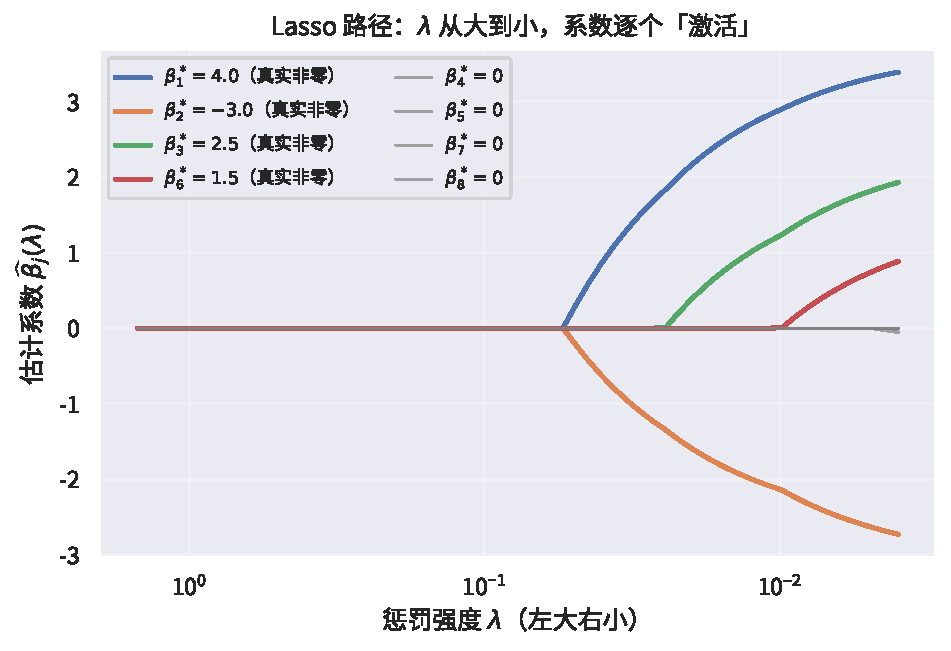
\includegraphics[width=0.85\linewidth]{figures/ch6_lassopath.pdf}
  \caption{Lasso 正则化路径（模拟数据，真实系数 $4,-3,2.5,0,0,1.5,0,0$）：$\lambda$ 从大到小（横轴左大右小），四个真实非零系数（彩线）依次从 $0$ 被「激活」，真实为零的系数（灰线）始终被压在 $0$ 附近——稀疏性不是假设出来的，是 $\ell_1$ 惩罚的几何（菱形约束角）自动选择的。}
  \label{fig:ch6-lassopath}
\end{figure}

\subsection{推断：debiased lasso 与条件独立的检验}\label{sec:debiased}

估计给出 $\hat\beta_j$ 之后，\textbf{点估计不能直接变成 $p$ 值}：lasso 的收缩使 $\hat\beta_j$ 有偏，其极限分布不是高斯。出路是\textbf{去偏}（debiasing / desparsifying）。思想一句话：\textit{把被惩罚偷走的项加回来}。取精度矩阵的 nodewise 估计 $\widehat{\bm{\Theta}}$（例如对 $\bm{S}$ 的每个节点做 lasso 回归、或直接用 CLIME），定义
\begin{equation}\label{eq:debiased}
  \widetilde{\bbeta} = \widehat{\bbeta}_{\mathrm{lasso}} + \tfrac{1}{n}\, \widehat{\bm{\Theta}}\, \X^\top \big( \y - \X \widehat{\bbeta}_{\mathrm{lasso}} \big).
\end{equation}
代数上看（练习 \ref{ex:debiased}）：$\widetilde{\bbeta} - \bbeta = \frac{1}{n}\widehat{\bm{\Theta}}\X^\top \bm{\varepsilon} + (\bm{I} - \widehat{\bm{\Theta}}\bm{S})(\bbeta - \widehat{\bbeta}_{\mathrm{lasso}})$——第一项是噪声（渐近正态），第二项是残余偏差（在稀疏性条件下 $o_p(n^{-1/2})$）。于是（Zhang \& Zhang, 2014; van de Geer et al., 2014）
\begin{equation}\label{eq:asym-norm}
  \sqrt{n}\, \big( \widetilde{\beta}_j - \beta_j \big) \ \xrightarrow{d}\ \mathcal{N}\Big( 0,\ \sigma^2 \big( \bm{\Theta}\, \bm{\Sigma}\, \bm{\Theta} \big)_{jj} \Big),
  \qquad
  \text{置信区间：}\ \widetilde{\beta}_j \pm z_{1-\alpha/2}\, \frac{\hat\sigma}{\sqrt{n}} \sqrt{ \big( \widehat{\bm{\Theta}}\, \bm{S}\, \widehat{\bm{\Theta}} \big)_{jj} } .
\end{equation}
\cite{zhang2014,vandegeer2014} 高维下对单个系数的\textbf{渐近正态推断}就此恢复——而由 \eqref{eq:beta-theta}，检验 $H_0: \beta_j = 0$ 正是\textbf{检验 $y$ 与 $x_j$ 的条件独立性}。整条流水线收拢为：

\begin{keybox}[from estimate to inference]
\[
\begin{gathered}
\underbrace{\text{lasso / elastic net / CLIME / glasso 估计 }\bm{\Theta},\bbeta}_{\text{第 \ref{sec:ggm-estimate} 节：稀疏点估计（有偏、快）}}
\\[1.2ex]
\Big\downarrow
\\[0.6ex]
\underbrace{\text{debias：}\widetilde{\bbeta} = \widehat{\bbeta} + \tfrac1n\widehat{\bm{\Theta}}\X^\top(\y - \X\widehat{\bbeta})}_{\text{把惩罚偷走的偏差加回来}}
\\[1.2ex]
\Big\downarrow
\\[0.6ex]
\underbrace{\text{渐近正态 \eqref{eq:asym-norm} $\Rightarrow$ 置信区间 / } H_0:\beta_j=0 \Leftrightarrow y \perp x_j \mid \x_{-j}}_{\text{条件独立检验，进而（在图假设下）因果读法}}
\end{gathered}
\]
估计回答「哪些边可能存在」，推断回答「这条边是否显著到不能归因于噪声」；二者之间隔着一次 debias——这是高维统计从「预测」走向「科学断言」的标准路径。
\end{keybox}

\textit{单个}系数的 $p$ 值之外，应用科学家面对的是 $d$ 个系数同时被检验的一整页结论——「这一页里有几个是真的」成为新的问题。多重检验的错误发现率控制（BH 程序、knockoffs）是第 \ref{sec:fdr} 章的主题，也是稀疏性故事在检验问题上的闭环。

\begin{exercise}\label{ex:block-inv}
分块求逆：对 $\bm{\Sigma} = \begin{pmatrix} \Sigma_{yy} & \bm{\Sigma}_{yX} \\ \bm{\Sigma}_{Xy} & \bm{\Sigma}_{XX} \end{pmatrix}$，用 $\bm{\Theta} = \bm{\Sigma}^{-1}$ 的分块验证 \eqref{eq:conditional} 与 \eqref{eq:beta-theta}，并推导偏相关公式 \eqref{eq:ci-prec}。
\end{exercise}

\begin{exercise}\label{ex:debiased}
推导 \eqref{eq:debiased} 的误差分解 $\widetilde{\bbeta} - \bbeta = \frac{1}{n}\widehat{\bm{\Theta}}\X^\top\bm{\varepsilon} + (\bm{I} - \widehat{\bm{\Theta}}\bm{S})(\bbeta - \widehat{\bbeta}_{\mathrm{lasso}})$，并解释两项分别为何是「方差」与「偏差」。
\end{exercise}

\begin{exercise}\label{ex:glasso-clime}
比较 graphical lasso 与 CLIME 的最优性条件：前者把「$\bm{\Theta}$ 是 $\bm{S}$ 之逆」写成 $\bm{S} - \bm{\Theta}^{-1} + \lambda\bm{\Gamma} = \zero$（依赖 $\bm{\Theta}$ 正定可逆），后者写成 $\bm{S}\bm{\Theta} - \bm{I} \approx \zero$（线性约束）。讨论：当 $d \gg n$、$\bm{S}$ 高度病态时，哪一种的优化问题更良态？CLIME 的逐列线性规划结构还带来什么实际好处？
\end{exercise}

\clearpage
% 第 7 章
\section{规模化推断：错误发现率控制（FDR）}\label{sec:fdr}

第 \ref{sec:debiased} 节把单个系数 $\beta_j$ 的点估计升级成了 $p$ 值。但应用科学家从不只检验一个假设：一次基因组筛选同时检验 $d \approx 2\times 10^4$ 个基因，一次营销复盘同时看几百个细分指标，一次流行病学分析对几十种暴露各做一次回归。\textbf{第 6 章回答「这一个系数显著吗」；本章回答「这一整页结论里，有几个是真的」}——这是把回归输出变成\textbf{可信的科学断言}之前的最后一英里，也是从稀疏估计走向 FDR 控制的闭环。

\subsection{问题的起点：多重检验与「发现的可信度」}\label{sec:fdr-problem}

设有 $m$ 个假设 $H_1, \dots, H_m$（例如 $H_j: \beta_j = 0$），对应 $p$ 值 $p_1, \dots, p_m$，其中 $m_0$ 个为真。对每个 $p$ 值各自做水平 $\alpha$ 的检验，若全部 $m_0$ 个零假设为真，至少误拒一个的概率高达
\[
  1 - (1 - \alpha)^{m_0} \ \approx\ 1 - e^{-\alpha m_0}
  \qquad (m_0 \text{ 大时几乎必然发生}).
\]
$m = 10^4$、$\alpha = 0.05$ 时几乎为 $100\%$（$1 - 0.95^{10^4} \approx 1 - e^{-513}$）——\textbf{「这一页里全是假的」不是意外，是默认结局}。

古典的补救是控制\textbf{族错误率}（Family-Wise Error Rate, FWER）：$\mathrm{FWER} = \Prob( V \ge 1 )$，其中 $V$ = 误拒（假发现）的个数。Bonferroni 方法把每个检验的阈值压到 $\alpha/m$：FWER $\le \alpha$ 确实成立，但代价是\textbf{阈值随 $m$ 线性收紧}。$m = 10^4$ 时阈值是 $5\times 10^{-6}$：除非效应巨大，否则\emph{什么也拒绝不了}——控制住了错误，也控制住了发现。

Benjamini 与 Hochberg 在 1995 年提出了一个更符合「筛查」场景的问题\cite{benjamini1995}：不要承诺「一个都不错」，而是控制\textbf{错误发现率}（False Discovery Rate）
\begin{equation}\label{eq:fdr-def}
  \mathrm{FDR} = \E\Big[ \frac{V}{\max(R, 1)} \Big],
  \qquad R = \text{拒绝总数}.
\end{equation}
$V/R$ 是\textbf{被拒绝者中假发现的比例}（$R = 0$ 时约定为 $0$）。FDR 允许「有假发现」，但要求其在\textbf{比例}意义下受控——发现得越多，容忍的假发现越多；一个都拒绝不了时也不欠任何债。FWER 与 FDR 的关系是一行字（练习 \ref{ex:bh-bonf}）：
\[
  \mathrm{FDR} \le \mathrm{FWER},
\]
所以控制 FWER 的 Bonferroni 必然控制 FDR——只是太保守。两者的适用分工因此清晰：\textbf{确证性}场景（一个断言上法庭、上说明书）要 FWER；\textbf{探索性}场景（筛选候选基因、圈定重点指标）该用 FDR。

\subsection[Benjamini--Hochberg 程序：斜线与最后一个交叉点]{Benjamini--Hochberg 程序：排序、斜线与最后一个交叉点}\label{sec:bh}

BH 程序的构造出人意料地简单。把 $p$ 值排序 $p_{(1)} \le \dots \le p_{(m)}$，给定目标水平 $q \in (0, 1)$，定义
\begin{equation}\label{eq:bh}
  \hat{k} = \max\Big\{ k :\ p_{(k)} \le \frac{q\, k}{m} \Big\},
  \qquad
  \text{拒绝 } H_{(1)}, \dots, H_{(\hat{k})}
  \ \ \text{（$\hat{k}$ 不存在则不拒绝任何假设）}.
\end{equation}
几何上看（图 \ref{fig:ch7-fdr}(a)）：把排序后的 $p$ 值画成阶梯，与斜线 $qk/m$ 找\textbf{最后一个交叉点}。Bonferroni 是水平线 $q/m$（只看 $k=1$ 一个点），BH 把阈值随次序 $k$ \emph{线性放松}——第 $k$ 小的 $p$ 值面临的门槛是 Bonferroni 的 $k$ 倍。

\begin{theorem}[Benjamini--Hochberg, 1995]\label{thm:bh}
若 $p$ 值相互独立，或更一般地满足正相关性条件（PRDS），则 BH 程序 \eqref{eq:bh} 满足
\[
  \mathrm{FDR} \le \frac{m_0}{m}\, q \ \le\ q .
\]
\end{theorem}
独立情形的完整证明是练习 \ref{ex:bh-proof} 的引导式归纳；这里给直觉。假发现的比例由「斜线的斜率」裁决：$qk/m$ 这条线的\textbf{放松速率}恰好是每拒绝 $k$ 个、最多容忍 $qk$ 个假的。真实的假发现进入拒绝集的方式是「混在真信号里的小 $p$ 值」，而当真实信号存在时，$\hat{k} \gg 1$，阈值 $q\hat{k}/m$ 相对 $q/m$ 放松了两个数量级——\textbf{发现越多，单个假设的门槛越宽松，但宽松的总预算被 $q$ 锁死}。这正是「在发现多的前提下容忍少量假的」的精确机制。

\begin{figure}[htbp]
  \centering
  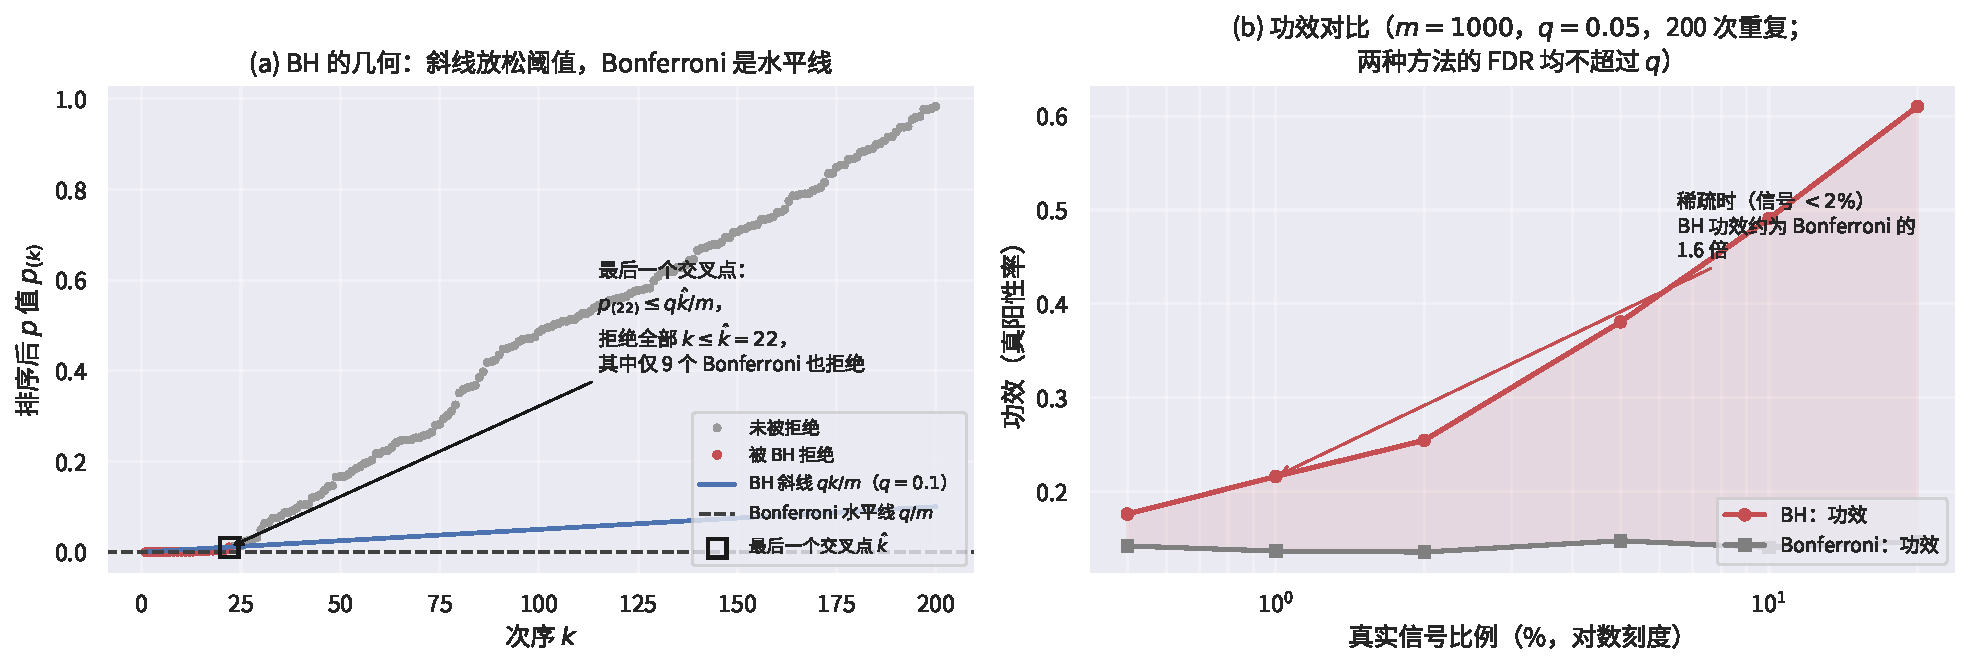
\includegraphics[width=\linewidth]{figures/ch7_fdr.pdf}
  \caption{(a) BH 的几何（一次模拟：$m=200$ 个独立检验，其中 30 个信号 $z_j \sim \mathcal{N}(3.2, 1)$，$q=0.1$）：排序 $p$ 值阶梯与斜线 $qk/m$ 的最后一个交叉点在 $\hat{k}=22$，拒绝全部 $k\le 22$；Bonferroni 的水平线 $q/m$ 只拒绝其中 9 个。(b) 功效模拟（$m=1000$，$q=0.05$，200 次重复）：信号比例从 $0.5\%$ 到 $20\%$（$z_j \sim \mathcal{N}(3,1)$），BH 的功效从 $0.18$ 升到 $0.61$，Bonferroni 的水平线被钉死在 $0.14$ 附近；信号比例为 $1\%$ 时 BH 功效约为 Bonferroni 的 $1.6$ 倍。两种方法的 FDR 实测均不超过 $q$（BH 在 $0.038$--$0.054$ 之间，Bonferroni 在 $0.0008$--$0.045$ 之间）——\textbf{斜线买到的功效没有多花一分钱错误率}。}
  \label{fig:ch7-fdr}
\end{figure}

\subsection{闭环：BH 是自适应的稀疏估计器}\label{sec:fdr-sparsity}

现在回到本书的主线——稀疏性。把单尾 $p$ 值换成 $z$ 分数 $z_j = \Phi^{-1}(1 - p_j)$，BH 程序等价于在有序 $z$ 分数上找一个\textbf{数据驱动的截断点}：拒绝 $z_{(j)} \ge \hat{t}$ 的假设。这个截断点不是预先给定的 $\sqrt{2 \log m}$，而是由数据自己「长」出来的——它长在哪里，取决于信号有多稀疏。

Abramovich、Benjamini、Donoho 与 Johnstone（2006）把这层观察变成了定理\cite{abramovich2006}。考虑稀疏正态均值模型
\[
  z_j = \theta_j + \varepsilon_j, \qquad \varepsilon_j \sim \mathcal{N}(0, 1),
  \qquad \#\{ j : \theta_j \neq 0 \} \le s \ll m,
\]
把 BH 在适当水平 $q$ 下的截断当作\emph{阈值估计器} $\hat\theta_j = z_j \cdot \ind{ z_j \ge \hat{t} }$（硬阈值）。其核心结论：\textbf{在稀疏度 $s$ 未知的情况下，这个由 FDR 控制规则定义的估计器自动达到与「知道 $s$」的 oracle 阈值相同的 minimax 风险率}——平方风险量级为 $2 s \log(m/s)$（相差常数因子），而不是非自适应阈值 $\sqrt{2 \log m}$ 给出的 $2 s \log m$。当 $s \ll m$ 时，$\log(m/s) \ll \log m$，这个差距是实质性的。

与第 \ref{sec:ggm-estimate} 节并排看，同一张面孔出现了两次：
\begin{center}
\begin{tabular}{@{}lll@{}}
\toprule
 & 稀疏估计（第 6 章） & FDR 检验（本节） \\
\midrule
对象 & 回归系数 $\bbeta$ 或均值 $\bm{\theta}$ & 一族假设 $H_1, \dots, H_m$ \\
机制 & $\ell_1$ 惩罚 / 软阈值 & 排序 $p$ 值 / BH 阈值 \\
自适应来源 & 惩罚参数 $\lambda$ 由交叉验证或 BIC & 截断点由斜线交叉自动定位 \\
稀疏性的角色 & 使估计在 $d \gg n$ 下仍可能 & 使 BH 阈值自动降到信号层 \\
\bottomrule
\end{tabular}
\end{center}
\textbf{控制假发现率不是估计之外的补丁，而是稀疏性假设在检验问题上的对偶表述}：「大多数系数是零」既让 lasso 能估计，也让 BH 能自适应地找到阈值。Donoho 的名字在第 6 章（压缩感知传统）与本节各出现一次，不是巧合——这是同一条「稀疏性 $\Rightarrow$ 阈值 $\Rightarrow$ 最优性」逻辑链的两端。

\subsection[回到回归 I：debiased lasso 的 $p$ 值与 BH]{回到回归 I：debiased lasso 的 $p$ 值经 BH，即控制系数的 FDR}\label{sec:fdr-regression}

流水线已经就位：第 \ref{sec:debiased} 节给出 $\sqrt{n}(\widetilde{\beta}_j - \beta_j)$ 的渐近正态性 \eqref{eq:asym-norm}，于是每个 $H_{0j}: \beta_j = 0$ 都有渐近 $p$ 值 $p_j$。把 $d$ 个 $p$ 值喂给 BH \eqref{eq:bh}，按定理 \ref{thm:bh}——只要 $p$ 值近似独立或正相关——\textbf{被拒绝的系数集合的假发现率就被控制在 $q$}。结合第 \ref{sec:beta-theta} 节的对应 $\beta_j = 0 \Leftrightarrow y \perp x_j \mid \x_{-j}$，这就是高维回归里「条件独立结构筛选」的标准终点：lasso 选候选边、debiased lasso 出 $p$ 值、BH 控可信度。

诚实的保留有三条，按本书惯例逐条披露：
\begin{enumerate}[label=(\roman*)]
  \item \textbf{$p$ 值是渐近的}。\eqref{eq:asym-norm} 是 $n \to \infty$ 的极限陈述，有限样本下 BH 的控制是近似的；$d$ 相对 $n$ 越大，近似越需要靠稀疏性条件托底。
  \item \textbf{相关性结构}。debiased 的 $p$ 值之间由设计矩阵的相关性决定。极端共线（第 \ref{sec:hd-break} 节的病态）可能破坏 PRDS 条件，实测 FDR 可以超调；一般相关下有更保守的 Benjamini--Yekutieli 修正\cite{benjamini2001}（把 $q$ 换成 $q / \sum_{j=1}^m j^{-1} \approx q / \log m$），代价是功效。
  \item \textbf{筛选与推断的对象一致性问题}。若用 lasso 先筛掉一部分变量、只对幸存者做检验，标准的 BH 理论不再直接适用（选择本身引入了额外随机性）——这正是下一节方法要绕开的坑。
\end{enumerate}

\subsection[回到回归 II：Knockoffs]{回到回归 II：Knockoffs——不依赖 $p$ 值的 FDR 控制}\label{sec:knockoffs}

Barber 与 Candès（2015）换了一条更彻底的路\cite{barber2015}：\textbf{不去造 $p$ 值再校正，而是在设计矩阵里人为构造「影子变量」，让对称性本身成为控制的支点}。对每列 $\x_j \in \R^n$，构造影子（knockoff）$\tilde{\x}_j$，使得\textbf{交换任意一对 $(\x_j, \tilde{\x}_j)$ 后，增广设计矩阵 $[\X\ \tilde{\X}]$ 的联合分布不变}（交换性）。高斯设计下有显式构造——它需要 $\X$ 列相关的二阶信息，即\textbf{又回到了第 \ref{sec:cov-prec} 节的协方差/精度矩阵}：影子变量按相关性「补齐」原变量，相关越强的变量，其影子越能以假乱真。（口径注记：原始 Barber--Candès 的\textbf{固定-$X$} 构造要求 $n \ge 2d$；本书描述的按二阶信息构造影子是 \textbf{model-X} 高斯版本，其高维构造至今仍是活跃研究方向。）

接着定义每个变量的特征重要性 $Z_j$ 与其影子的重要性 $\tilde{Z}_j$（例如 lasso 路径上该变量进入模型的次序），合成\textbf{带符号统计量}
\[
  W_j = Z_j - \tilde{Z}_j ,
\]
约定 $W_j$ 的符号表示「原变量胜过影子」。关键观察：在 $H_{0j}$（$\x_j$ 与 $\y$ 无关）下，$\x_j$ 与影子毫无差别，交换性给出
\begin{equation}\label{eq:knockoff-sym}
  W_j \ \overset{d}{=}\ -W_j
  \qquad (H_{0j} \text{ 下，以其他变量为条件}),
\end{equation}
即\emph{零假设变量的 $W_j$ 关于 $0$ 对称}，而真实信号变量的 $W_j$ 倾向于取大正值。于是「负 $W$ 的个数」就成了「假发现的个数」的\textbf{对称性估计}：按 $|W_j|$ 从大到小， knockoff+ 程序取阈值
\begin{equation}\label{eq:knockoff}
  T = \min\Big\{ t > 0 :\ \frac{ 1 + \#\{ j : W_j \le -t \} }{ \#\{ j : W_j \ge t \} } \le q \Big\},
  \qquad
  \text{拒绝 } \{ j : W_j \ge T \}.
\end{equation}
分子里那个「$1+$」是对随机性的过离散校正；而 \eqref{eq:knockoff-sym} 保证每个被误拒的变量以 $1/2$ 的概率贡献一个负镜像——这正是定理证明的支点。结论：在任意模型（不需要线性、不需要渐近）下，
\[
  \mathrm{FDR} \le q .
\]

两条路线并排看，各司其职：
\begin{center}
\begin{tabular}{@{}lll@{}}
\toprule
 & BH + debiased lasso（第 \ref{sec:fdr-regression} 节） & Knockoffs（本节） \\
\midrule
控制支点 & $p$ 值的渐近正态性 & 设计矩阵的交换对称性 \\
模型假设 & 需要（线性 + 稀疏 + 渐近） & 不需要（模型无关） \\
有限样本保证 & 近似（渐近成立） & \textbf{精确}（有限样本） \\
额外代价 & debias 需要的 nodewise 估计 & 构造影子变量（固定-$X$ 构造需 $n \ge 2d$；model-X 需已知或可估特征分布） \\
\bottomrule
\end{tabular}
\end{center}

至此，「可信的科学断言」三件套齐备：debiased lasso 给\textbf{单个}系数的 $p$ 值（第 \ref{sec:debiased} 节），BH 给\textbf{一页} $p$ 值的 FDR 控制（本节之前），knockoffs 给\textbf{变量选择}的、模型无关的 FDR 控制（本节）。Candès 与 Donoho 在前言里被致敬，是因为回归的现代可信度理论恰好由他们两脉写成——一个负责「稀疏使估计可能」，一个负责「对称使推断可信」。

\begin{keybox}[本章要点]
\begin{itemize}
  \item 多重检验下 Bonferroni 控制 FWER 但阈值 $\alpha/m$ 随 $m$ 线性收紧、功效崩塌；FDR $= \E[V/\max(R,1)]$ 允许「发现多时容忍少量假的」，是探索性筛选的正确货币（\ref{sec:fdr-problem} 节）；
  \item BH 程序 $=$ 排序 $p$ 值与斜线 $qk/m$ 的最后一个交叉点；独立（或 PRDS）下 $\mathrm{FDR} \le q\, m_0/m \le q$（定理 \ref{thm:bh}）；
  \item 闭环：BH 阈值是对 $z$ 分数的自适应稀疏估计，稀疏度未知时达到 oracle 级别的 minimax 率\cite{abramovich2006}——控制假发现率与稀疏估计是同一枚硬币；
  \item 回归流水线：debiased lasso 出 $p$ 值、BH 控 FDR——但渐近近似与共线性是诚实披露的弱点；knockoffs 用影子变量的交换对称性给出模型无关、有限样本精确的 FDR 控制\cite{barber2015}。
\end{itemize}
\end{keybox}

\begin{exercise}\label{ex:bh-hand}
$m = 5$、$q = 0.1$，五个 $p$ 值（已排序）为 $0.001,\ 0.02,\ 0.04,\ 0.09,\ 0.3$。逐步执行 BH：写出每个 $k$ 的阈值 $qk/m$、判定、$\hat{k}$ 与最终拒绝集；再与 Bonferroni（阈值 $q/m$）及「逐个检验水平 $q$」三者的拒绝集比较。
\end{exercise}

\begin{exercise}\label{ex:bh-bonf}
(a) 证明 $\mathrm{FDR} \le \mathrm{FWER}$，并由此得出「控制 FWER 的任何程序（如 Bonferroni）必然控制 FDR」；(b) 证明 Bonferroni 在水平 $q$ 下的拒绝集是 BH 在水平 $q$ 下拒绝集的子集；(c) 设 $m = 10^5$ 个独立检验，其中 $200$ 个信号的 $z_j \sim \mathcal{N}(5, 1)$（双侧 $p$ 值），$q = 0.05$。估计 Bonferroni 的每检验阈值与功效，说明 BH 在 $\hat{k} \approx 200$ 处的阈值比它宽松多少、以及为什么此时 BH 的功效趋近 $1$ 而 Bonferroni 远不至此。
\end{exercise}

\begin{exercise}[证明梗概，较难]\label{ex:bh-proof}
在\textbf{全部 $m$ 个假设为真}且 $p$ 值\textbf{相互独立}的条件下，证明 $\Prob( \exists k : p_{(k)} \le qk/m ) \le q$（全零时 $\mathrm{FDR}$ 等于这个概率，故定理 \ref{thm:bh} 的最坏情形成立）。按以下骨架补全：(i) 对 $m$ 归纳，$m = 1$ 显然；(ii) 关键一步：以最大次序统计量 $p_{(m)}$ 是否 $\le q$ 分情况，利用「固定 $p_{(m)} = u$ 时，其余 $m-1$ 个是 $m-1$ 个独立 $U(0, u)$ 变量除以 $u$」的事实，把事件改写成关于 $m-1$ 个均匀变量的同类事件，并验证水平参数从 $q$ 变成 $q/u \cdot (u) = q$ 的恒等；(iii) 合并两种情况。
\end{exercise}

\begin{exercise}\label{ex:knockoff}
(a) 由交换性严格说明：在 $H_{0j}$ 下，把 $\x_j$ 与 $\tilde{\x}_j$ 全局交换后统计量向量 $(W_1, \dots, W_m)$ 的联合分布不变，而这使 $W_j$ 变号——由此得出 \eqref{eq:knockoff-sym}（提示：$H_{0j}$ 下 $\y$ 不依赖 $\x_j$，交换不改变回归问题）；(b) 解释为什么 \eqref{eq:knockoff} 分母里的 $\#\{j : W_j \ge t\}$ 是「$|W|$ 超过 $t$ 的发现数」，而分子（除 $1+$ 外）的 $\#\{j : W_j \le -t\}$ 是它的\textbf{假发现数估计}——对称性如何把这个估计变成上界期望的支点。
\end{exercise}

\clearpage
% 第 8 章
\section{非线性的潜空间：线性回归作为天然的核方法}\label{sec:kernel}

第 \ref{sec:intro} 章说过：「线性」是对\textbf{参数}的要求，不是对原始变量的要求。本章把这句话推到极限：设观测到的特征其实是高维潜变量的非线性投影
\begin{equation}\label{eq:feature-map}
  \x_i = \phi(\bm{z}_i), \qquad \bm{z}_i \in \R^q \ \text{(潜变量)}, \quad \phi : \R^q \to \R^d \ \text{(特征映射)},
\end{equation}
其中维度 $d$ 可以任意大——包括无穷大。对 $\y = \X \bbeta + \bm{\varepsilon}$ 做最小二乘，就是把第 \ref{sec:highdim}--\ref{sec:gd-underdet} 章的全部机器开在 $\bm{\Phi} := [\phi(\bm{z}_1)^\top; \dots; \phi(\bm{z}_n)^\top] \in \R^{n \times d}$ 上。本章的核心结论是：\textbf{$\X$ 与 $\y$ 之间的线性回归，在潜变量 $\bm{z}$ 的世界里表现为一个核方法（kernel method）——预测对 $\bm{z}$ 是非线性的，而计算只需要 $n \times n$ 的核矩阵}。

\subsection{核函数与 Gram 矩阵：把内积当作唯一接口}\label{sec:kernel-def}

定义\textbf{核函数}为特征空间中的内积
\begin{equation}\label{eq:kernel}
  k(\bm{z}, \bm{z}') = \big\langle \phi(\bm{z}),\ \phi(\bm{z}') \big\rangle ,
\end{equation}
以及样本 Gram 矩阵与新样本的核向量
\begin{equation}\label{eq:gram}
  \bm{K} = \bm{\Phi} \bm{\Phi}^\top \in \R^{n \times n},
  \qquad
  K_{ij} = k(\bm{z}_i, \bm{z}_j);
  \qquad
  \bm{k}(\bm{z}) = \bm{\Phi}\, \phi(\bm{z}) = \big( k(\bm{z}, \bm{z}_1), \dots, k(\bm{z}, \bm{z}_n) \big)^\top .
\end{equation}
注意 \eqref{eq:gram} 中\textbf{没有出现任何 $\phi$ 的坐标}——核方法的全部思想就是：如果算法的每个中间量都能用内积 $\langle \phi(\cdot), \phi(\cdot)\rangle$ 表达，那么 $\phi$ 永远不需要被显式构造，$d = \infty$ 也无所谓。 Mercer 定理保证：任何正定核 $k$ 都对应某个（可能无穷维的）特征映射 $\phi$，二者是同一对象的两张脸\cite{scholkopf2002}。

\subsection[$d > n$：欠定闭式解的核形式]{$d > n$：$\widehat{\bbeta}'$ 的核形式}\label{sec:kernel-underdet}

把第 \ref{sec:gd-underdet} 章的欠定闭式解 $\widehat{\bbeta}' = \X^\top(\X\X^\top)^{-1}\y$ 中的 $\X$ 换成 $\bm{\Phi}$。对新样本 $\tilde{\x} = \phi(\tilde{\bm{z}})$，预测为
\begin{equation}\label{eq:kernel-interp}
  \tilde{\x}^\top \widehat{\bbeta}'
  = \phi(\tilde{\bm{z}})^\top \bm{\Phi}^\top (\bm{\Phi}\bm{\Phi}^\top)^{-1} \y
  = \bm{k}(\tilde{\bm{z}})^\top \bm{K}^{-1} \y .
\end{equation}
逐步检查这一行里的每个对象：$\bm{\Phi}\bm{\Phi}^\top = \bm{K}$ 是核矩阵；$\phi(\tilde{\bm{z}})^\top \bm{\Phi}^\top = \bm{k}(\tilde{\bm{z}})^\top$ 是核向量。\textbf{预测被完全写成了核函数的形式}。进一步写成展开式
\begin{equation}\label{eq:kernel-expansion}
  \hat{f}(\tilde{\bm{z}}) = \tilde{\x}^\top \widehat{\bbeta}' = \sum_{i=1}^n \alpha_i\, k(\tilde{\bm{z}}, \bm{z}_i),
  \qquad
  \bm{\alpha} = \bm{K}^{-1} \y ,
\end{equation}
即预测是\textbf{以训练点为锚点的核截面的线性组合}——这就是\textbf{核插值}（kernel interpolation），也称 kernel ridgeless regression：它是 $d > n$ 特征空间里最小范数插值解（第 \ref{sec:minnorm} 节）在核语言中的样子，而对正定核而言特征空间范数恰是 RKHS 范数——\textbf{GD 从零点收敛到的点，同时是 RKHS 中范数最小的插值函数}\cite{kimeldorf1970}。这就是用户问题中 $(\phi(\bm{Z})\phi(\bm{Z})^\top)^{-1}$ 的核写法：\textit{它不需要被构造——它就是 $\bm{K}^{-1}$，由核函数值直接组装}。

\subsection[$n \gg d$：OLS 闭式解的核形式]{$n \gg d$：$\bhat$ 的核形式与 push-through 恒等式}\label{sec:kernel-overdet}

把第 \ref{sec:hd-closed} 节的 $\bhat = (\X^\top\X)^{-1}\X^\top\y$ 中的 $\X$ 换成 $\bm{\Phi}$，预测为 $\phi(\tilde{\bm{z}})^\top (\bm{\Phi}^\top\bm{\Phi})^{-1} \bm{\Phi}^\top \y$。问题来了：$\bm{\Phi}^\top\bm{\Phi} \in \R^{d \times d}$ 的元是 $\sum_i \phi_a(\bm{z}_i)\phi_b(\bm{z}_i)$——\textbf{特征坐标的交叉项，不能由核矩阵 $\bm{K}$ 单独决定}。这正是「什么时候能核化」的分界线：一切只依赖观测点两两内积的量可以核化，依赖特征坐标系本身的量不能。

出路是第 \ref{sec:hd-break} 节已经熟悉的 ridge——它既修复病态，又恰好完成核化。加 $\lambda$ 后的预测为 $\phi(\tilde{\bm{z}})^\top(\bm{\Phi}^\top\bm{\Phi} + \lambda \bm{I}_d)^{-1}\bm{\Phi}^\top\y$，用 \textbf{push-through 恒等式}（两边同乘 $(\bm{\Phi}^\top\bm{\Phi} + \lambda\bm{I})$ 即可验证）
\begin{equation}\label{eq:push-through}
  (\bm{\Phi}^\top\bm{\Phi} + \lambda \bm{I}_d)^{-1} \bm{\Phi}^\top
  = \bm{\Phi}^\top (\bm{\Phi}\bm{\Phi}^\top + \lambda \bm{I}_n)^{-1}
  = \bm{\Phi}^\top (\bm{K} + \lambda \bm{I}_n)^{-1},
\end{equation}
右端每个因子都是核对象。于是\textbf{核岭回归}
\begin{equation}\label{eq:kernel-ridge}
  \hat{f}(\tilde{\bm{z}}) = \bm{k}(\tilde{\bm{z}})^\top (\bm{K} + \lambda \bm{I}_n)^{-1} \y .
\end{equation}
这就是用户问题中 $(\phi(\bm{Z})^\top\phi(\bm{Z}))^{-1}$ 的核写法：\textit{它先被 $\lambda$ 正则化，再经 push-through 翻转到样本空间，成为 $(\bm{K} + \lambda\bm{I}_n)^{-1}$——原始空间里的 $d \times d$ 逆，从未被计算}。令 $\lambda \to 0^+$，\eqref{eq:kernel-ridge} 形式上回到 \eqref{eq:kernel-interp}：\textbf{两个 regime 在核语言里殊途同归}。高斯过程回归是同一个对象的贝叶斯叙述（核 = 协方差函数，后验均值 = \eqref{eq:kernel-ridge}）\cite{scholkopf2002}。

\subsection{例子：什么时候核是「天然」的}\label{sec:kernel-examples}

\begin{itemize}
  \item \textbf{多项式核} $k(\bm{z}, \bm{z}') = (\bm{z}^\top \bm{z}' + c)^m$：对应显式有限维特征映射（全体阶数 $\le m$ 的单项式），$d = \binom{q+m}{m}$——$n \gg d$ 的有限维回归，核化只是省事。
  \item \textbf{高斯核}（RBF）$k(\bm{z}, \bm{z}') = \exp\!\big( -\norm{\bm{z} - \bm{z}'}^2 / 2\sigma^2 \big)$：对应的 $\phi$ 是\textbf{无穷维}的，显式构造不可能——此时核化不是技巧而是\textit{唯一}出路。\eqref{eq:kernel-interp} 的 $d > n$ 故事天然属于这里。
  \item \textbf{随机特征}（Rahimi \& Recht, 2007）：反过来，用 $\phi(\bm{z}) = \sqrt{\tfrac{2}{D}}\big(\cos(\bm{\omega}_1^\top \bm{z} + b_1), \dots\big)$（随机频率）把高斯核近似回\textbf{有限}维、然后跑本章全部 $d$ 维线性代数——$d \to \infty$ 时随机特征回归收敛到核回归\cite{rahimi2007}。这条路把「核方法」与「宽神经网络」焊接在一起：随机特征回归正是两层无穷宽网络的函数空间极限的线性版本。
\end{itemize}

\begin{figure}[htbp]
  \centering
  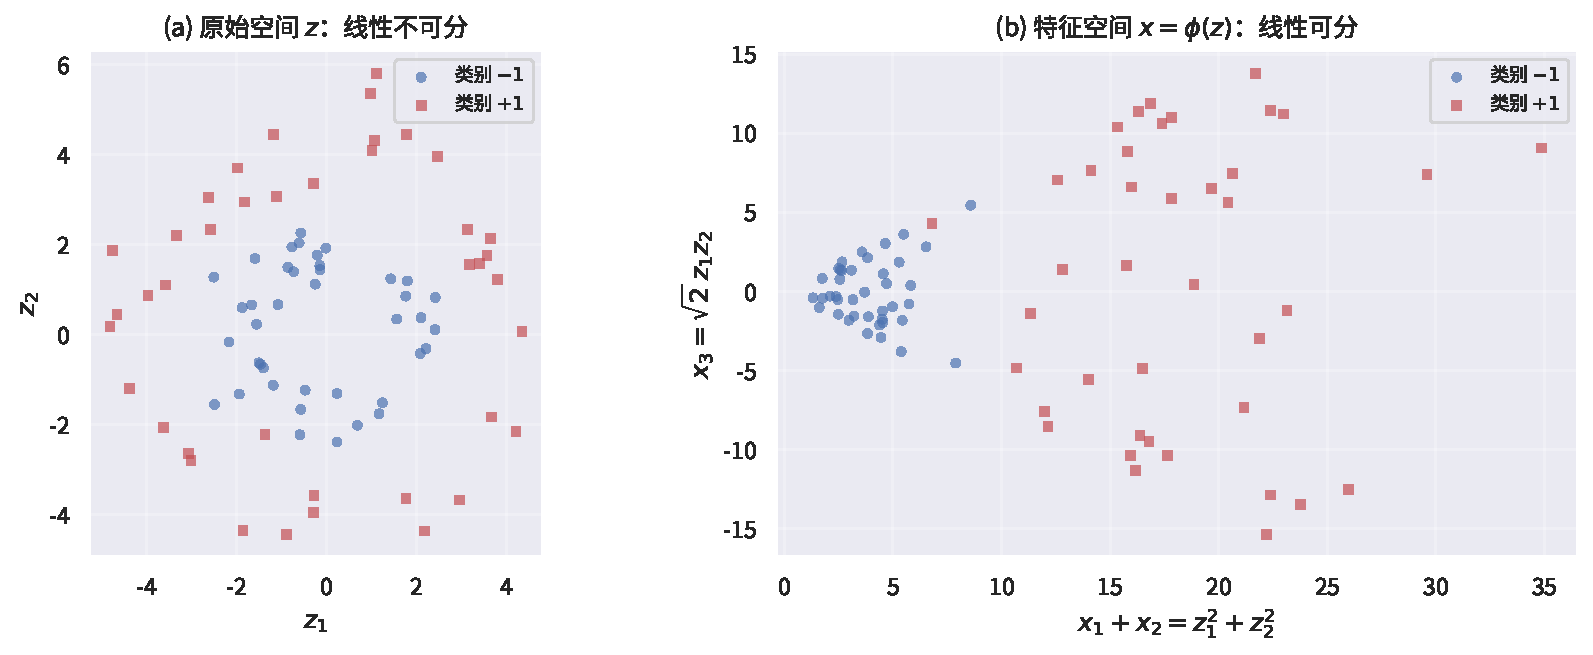
\includegraphics[width=\linewidth]{figures/ch7_kernel.pdf}
  \caption{核方法的几何本质：同一份环形数据（按半径分两类），在原始潜空间 $z$（左）里任何直线都分不开；经二次特征映射 $\phi(z)=(z_1^2, z_2^2, \sqrt{2}z_1z_2)$ 升到特征空间（右）后，一个线性函数即可分开。\textbf{对 $x$ 线性 $=$ 对 $z$ 非线性}——线性回归的预测由此成为潜空间中的天然非线性方法。}
  \label{fig:ch7-kernel}
\end{figure}

\subsection[从核回归到深度网络：Fourier 特征的 ridgeless 回归与 NTK]{从核回归到深度网络：ridgeless 回归、Fourier 特征与神经正切核}\label{sec:ntk}

本章最后做一件「收拢全书」的事：把「线性回归 $\to$ 核回归」这条路一直走到\textbf{深度神经网络}的门口。沿途有两座桥：第一座是\textbf{随机 Fourier 特征}（旧桥，2007），第二座是\textbf{神经正切核}（NTK，新桥，2018）\cite{jacot2018}。

\subsubsection*{桥一：两层网络 = 随机特征上的线性回归}

考虑最简单的两层网络
\begin{equation}\label{eq:two-layer}
  f(\bm{z}; \bm{a}) = \frac{1}{\sqrt{D}} \sum_{j=1}^{D} a_j\, \sigma\big( \bm{\omega}_j^\top \bm{z} + b_j \big),
\end{equation}
其中 $\sigma$ 是激活函数（ReLU、tanh 等），第一层参数 $(\bm{\omega}_j, b_j)$ 从某分布\textbf{随机采样后冻结}，只训练第二层 $\bm{a} \in \R^D$。注意两件事：

\begin{enumerate}[label=(\arabic*)]
  \item 定义 $\phi(\bm{z}) = \tfrac{1}{\sqrt{D}}\big(\sigma(\bm{\omega}_1^\top\bm{z}+b_1), \dots, \sigma(\bm{\omega}_D^\top\bm{z}+b_D)\big)^\top$，则 $f(\bm{z};\bm{a}) = \phi(\bm{z})^\top\bm{a}$——\textbf{它就是关于 $\bm{a}$ 的线性回归}，本章全部机器（正规方程、GD 精确解、push-through、核化判据）原封不动适用。
  \item 若 $\bm{a}$ 的初值取零且用梯度下降训练，第 \ref{sec:implicit} 章的隐式正则化分析说：它收敛到\textbf{最小范数}插值解——在 $\bm{a}$ 的 Euclidean 范数意义下。这就是\textbf{ridgeless 回归}（$\lambda \to 0^+$ 的 ridge，见练习 \ref{ex:ridge-dual}）：\textit{没有任何显式惩罚，插值解中范数最小的那个被 GD 自动选中}。
\end{enumerate}

由 \eqref{eq:kernel-interp}，其预测的核形式不变，只是核函数换成了\textbf{随机特征核}
\begin{equation}\label{eq:rf-kernel}
  k_{\mathrm{RF}}(\bm{z}, \bm{z}') = \frac{1}{D}\sum_{j=1}^D \sigma(\bm{\omega}_j^\top\bm{z}+b_j)\,\sigma(\bm{\omega}_j^\top\bm{z}'+b_j)
  \ \xrightarrow{D \to \infty}\ \E_{\bm{\omega}, b}\big[ \sigma(\bm{\omega}^\top\bm{z} + b)\,\sigma(\bm{\omega}^\top\bm{z}' + b) \big],
\end{equation}
这正是 Rahimi \& Recht 随机 Fourier 特征的理论核心（对移位不变核，取 $\sigma = \cos$ 与特定采样分布，\eqref{eq:rf-kernel} 精确重现高斯核）\cite{rahimi2007}。\textbf{一句话：冻结第一层、训练第二层、零初始化、梯度下降 $=$ Fourier 特征空间里的 ridgeless 回归。}

\subsubsection*{桥二：NTK——全部参数都训练时，函数空间仍是线性的}

桥一留了一个「不自然」的假设：第一层被冻结。如果\textbf{所有参数} $\bm{\theta} = (\bm{a}, \{ \bm{\omega}_j, b_j \})$ 都参与训练呢？参数空间的损失
\[
  L(\bm{\theta}) = \frac{1}{2}\sum_{i=1}^n \big( f(\bm{z}_i; \bm{\theta}) - y_i \big)^2
\]
关于 $\bm{\theta}$ 一般\textbf{非凸}——这正是深度学习「神秘」的出处。Jacot、Gabriel 与 Hongler 的关键观察是：别盯参数空间，盯\textbf{函数空间}。对训练集上的残差向量 $\bm{r}_t = \big( f(\bm{z}_i; \bm{\theta}_t) - y_i \big)_i$，链式法则给出
\begin{equation}\label{eq:ntk-flow}
  \frac{d\, f(\bm{z}; \bm{\theta}_t)}{dt}
  = \nabla_{\bm{\theta}} f(\bm{z}; \bm{\theta}_t)^\top \frac{d\bm{\theta}_t}{dt}
  = -\sum_{i=1}^n \underbrace{\big\langle \nabla_{\bm{\theta}} f(\bm{z}; \bm{\theta}_t),\ \nabla_{\bm{\theta}} f(\bm{z}_i; \bm{\theta}_t) \big\rangle}_{\Theta_t(\bm{z}, \bm{z}_i)} \, r_{t,i} ,
\end{equation}
其中
\begin{equation}\label{eq:ntk-def}
  \Theta_t(\bm{z}, \bm{z}') := \big\langle \nabla_{\bm{\theta}} f(\bm{z}; \bm{\theta}_t),\ \nabla_{\bm{\theta}} f(\bm{z}'; \bm{\theta}_t) \big\rangle
\end{equation}
称为\textbf{神经正切核}（Neural Tangent Kernel）。\eqref{eq:ntk-flow} 的形状你一定认得：它就是\textbf{函数空间里的核梯度下降}——与第 \ref{sec:gd} 章的 $\widehat{\bbeta}_{t+1} = \widehat{\bbeta}_t - \eta\,\X^\top(\X\widehat{\bbeta}_t - \y)$ 同构，只是「设计矩阵的内积」被换成了「参数梯度的内积」。

NTK 的惊人之处在于其\textbf{宽网络极限}：以 $\tfrac{1}{\sqrt{D}}$ 缩放（\eqref{eq:two-layer} 已如此），当宽度 $D \to \infty$ 时：

\begin{enumerate}[label=(\arabic*)]
  \item 初始化时 $\Theta_0$ 依大数定律收敛到一个\textbf{确定性核} $\Theta$（对两层网络可显式算出，见练习 \ref{ex:ntk}）；
  \item 训练\textbf{全程}中 $\Theta_t$ 保持不动（$\Theta_t \to \Theta$，不随 $\bm{\theta}_t$ 漂移）——参数走了很远，核纹丝不动；
  \item 于是 \eqref{eq:ntk-flow} 成为\textbf{线性}常微分方程 $\frac{df_t(\bm{z})}{dt} = -\sum_i \Theta(\bm{z},\bm{z}_i)\, r_{t,i}$，其解以 $\Theta$ 的特征方向指数收敛，极限为
  \begin{equation}\label{eq:ntk-ridgeless}
    f_\infty(\tilde{\bm{z}}) = \bm{\Theta}(\tilde{\bm{z}})^\top \bm{\Theta}^{-1} \y,
  \end{equation}
  其中 $\bm{\Theta} = \big(\Theta(\bm{z}_i,\bm{z}_j)\big)_{ij}$ 是 NTK 在训练点上的 Gram 矩阵，$\bm{\Theta}(\tilde{\bm{z}})$ 是新样本的核向量。
\end{enumerate}

\eqref{eq:ntk-ridgeless} 与本章的 \eqref{eq:kernel-interp} \textbf{逐符号同构}：无穷宽、全参数训练的两层（乃至任意深度\cite{lee2019}）神经网络，在梯度下降下的函数空间极限，就是\textbf{以 NTK 为核的 ridgeless 核回归}。参数空间的非凸性是一个「坐标系的幻象」——换到函数空间，深度网络训练就是第 5 章的最小范数插值故事。

\begin{keybox}[从一条直线到深度网络的桥]
\[
\begin{gathered}
\text{线性回归 } \xrightarrow{\ \phi\ } \text{ 核回归 } \xrightarrow[\text{显式化}]{\ \text{随机 Fourier 特征}\ } \text{ 有限维 ridgeless 回归} \\
\xrightarrow[\text{全参数训练、宽极限}]{\ \mathrm{NTK}\ } \text{ 深度网络的函数空间极限}
\end{gathered}
\]
四个箭头分别由本章第 \ref{sec:kernel-overdet} 节（push-through）、\eqref{eq:rf-kernel}（大数定律）、第 \ref{sec:implicit} 章（隐式正则化）与 \eqref{eq:ntk-ridgeless}（NTK 不动性）支撑。\textbf{线性回归不是深度学习的特例；深度学习的宽极限是线性回归的核化}——这就是为什么两百年前的这条直线，仍然是理解今天一切模型的最诚实的起点。
\end{keybox}

两点务实的注记。其一，NTK 描述的是「lazy training」\textit{懒惰训练} regime：参数初始化尺度大、训练位移小，网络「懒得」改变内部特征——真实深度学习中特征学习（feature learning）发生时 NTK 失效，此时理论仍在建设中（Jacot 本人区分 lazy regime 与 feature-learning regime 的后续工作即为此）。其二，ridgeless 插值\textbf{非但不坏、还可能更好}：Belkin 等人的 double descent 观察表明，现代过参数模型的测试误差在插值阈值之后继续下降\cite{belkin2019}——第 \ref{sec:minnorm} 章的最小范数解正是这一现象最干净的线性化身，Jingfeng Wu 等人的工作进一步证明最优提前停止的 GD 在统计意义下支配最优 ridge（见前言与文献）\cite{wu2025}。把这两条注记与 \eqref{eq:ntk-ridgeless} 放在一起，你就拿到了「为什么过参数化网络能泛化」这个问题的、目前最诚实的线性回答。

\begin{figure}[htbp]
  \centering
  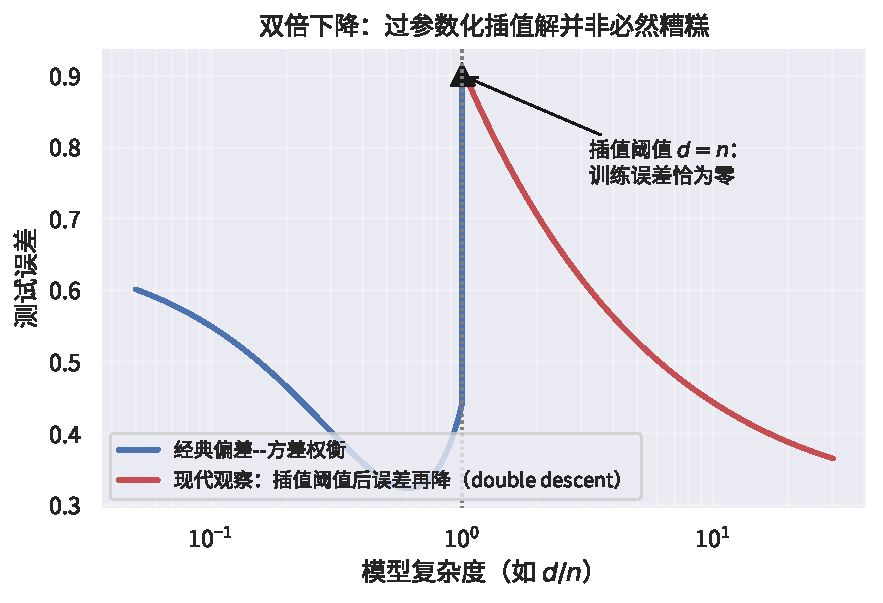
\includegraphics[width=0.72\linewidth]{figures/ch7_doubledescent.pdf}
  \caption{双倍下降（示意图；Belkin et al., 2019\cite{belkin2019}）：经典教科书说测试误差在 $d \approx n$ 处最优（蓝，U 型），现代观察发现误差在插值阈值 $d=n$ 处尖峰后\textbf{继续下降}（红）——插值本身不是罪，关键是插值解中隐式正则化选了哪一个。ridgeless 回归与提前停止的 GD 给出了这一选择的线性刻画。}
  \label{fig:ch7-doubledescent}
\end{figure}

\begin{exercise}\label{ex:ntk}
对 \eqref{eq:two-layer} 的两层网络（$\sigma$ 光滑），设 $(\bm{\omega}_j, b_j) \sim \mathcal{N}(\zero, \bm{I})$ i.i.d.，$\bm{a}$ 初值独立采样且 $\E[a_j^2] = 1$。验证：宽度 $D \to \infty$ 时，初始化处的 NTK \eqref{eq:ntk-def} 逐点收敛到
\[
  \Theta(\bm{z},\bm{z}') = \E\big[ \sigma(\bm{\omega}^\top\bm{z}+b)\,\sigma(\bm{\omega}^\top\bm{z}'+b) \big] \;+\; \bm{z}^\top\bm{z}'\, \E\big[ \sigma'(\bm{\omega}^\top\bm{z}+b)\,\sigma'(\bm{\omega}^\top\bm{z}'+b) \big],
\]
并指出两项分别来自「最后一层参数」与「第一层参数」的梯度；再说明第二项（随机特征核 \eqref{eq:rf-kernel} 中没有的那一项）为何使 NTK 严格强于随机特征核。对 $\sigma = \mathrm{ReLU}$，利用正态分布的半空间矩公式把两个期望写成 $\bm{z}$、$\bm{z}'$ 角度的显式函数。
\end{exercise}

\subsection{本章结论}\label{sec:kernel-conclusion}

\begin{keybox}[要点]
\begin{itemize}
  \item 设 $\x_i = \phi(\bm{z}_i)$，记 $\bm{K}_{ij} = k(\bm{z}_i,\bm{z}_j)$、$\bm{k}(\tilde{\bm{z}})_i = k(\tilde{\bm{z}}, \bm{z}_i)$，则
  \[
    d > n:\ \tilde{\x}^\top \widehat{\bbeta}' = \bm{k}(\tilde{\bm{z}})^\top \bm{K}^{-1} \y
    \ \xrightarrow{\ \lambda\ }\ 
    n \gg d:\ \tilde{\x}^\top \bhat^{\mathrm{ridge}} = \bm{k}(\tilde{\bm{z}})^\top (\bm{K} + \lambda \bm{I})^{-1} \y .
  \]
  线性回归的两个闭式解，都是\textbf{只用核函数组装的估计量}；
  \item 核化的关键两步：内积化（所有量写成 $\langle\phi,\phi\rangle$）与 push-through（$(\bm{\Phi}^\top\bm{\Phi} + \lambda\bm{I})^{-1}\bm{\Phi}^\top = \bm{\Phi}^\top(\bm{K} + \lambda\bm{I})^{-1}$）——后者把特征空间的逆翻转为样本空间的逆；
  \item 预测 $\hat{f}(\tilde{\bm{z}}) = \sum_i \alpha_i k(\tilde{\bm{z}}, \bm{z}_i)$ 对潜变量 $\bm{z}$ 是\textbf{非线性}的，尽管它对 $\x = \phi(\bm{z})$ 是线性的——「线性回归的预测是非线性潜空间映射下的天然核方法」，至此证毕；
  \item $d = \infty$（高斯核）时核化从便利变为必需；随机特征则反向地把核近似回有限维线性代数，连通过参数化网络。
\end{itemize}
\end{keybox}

\begin{exercise}\label{ex:kernel-dual}
用 \eqref{eq:push-through} 证明核岭回归的原始形式与对偶形式给出\textbf{完全相同}的预测函数，并解释为何 $\lambda > 0$ 时无需任何秩假设。
\end{exercise}

\begin{exercise}\label{ex:kernel-interp}
验证高斯核矩阵 $\bm{K}$（样本互异时）正定可逆，从而 \eqref{eq:kernel-interp} 有定义；进一步验证 \eqref{eq:kernel-expansion} 中的 $\bm{\alpha}$ 满足 $\bm{K}\bm{\alpha} = \y$（核插值方程），并把它与第 \ref{sec:gd-underdet} 章的插值验证 \eqref{eq:interp} 对应起来。
\end{exercise}

\clearpage
% 第 9 章
\section{结语：所以，为什么是线性回归？}\label{sec:epilogue}

把八条线索收拢。

\begin{figure}[htbp]
  \centering
  \begin{tikzpicture}[
      font=\small,
      box/.style={draw=blue!50!black, fill=blue!5, rounded corners=2pt,
                  align=center, inner sep=5pt, text width=3.5cm, minimum height=1.35cm},
      kern/.style={draw=green!45!black, fill=green!6, rounded corners=2pt,
                  align=center, inner sep=5pt, text width=3.5cm, minimum height=1.35cm},
      net/.style={draw=red!55!black, fill=red!5, rounded corners=2pt,
                  align=center, inner sep=5pt, text width=3.9cm, minimum height=1.35cm},
      arr/.style={->, >=Stealth, thick, gray!50!black},
      lab/.style={midway, font=\scriptsize, fill=white, inner sep=1.5pt}]
    \node[box] (onedim) at (0,0) {一维：斜率 $=$ 相关系数\\相关 vs 因果\\（第 2 章）};
    \node[box] (highdim) at (5.1,0) {高维闭式解：投影\\$\bhat=(\X^\top\X)^{-1}\X^\top\y$\\（第 3 章）};
    \node[box] (gd) at (10.2,0) {迭代视角：GD\\谱滤波、不动点\\（第 4 章）};
    \node[box] (under) at (10.2,-2.7) {欠定：最小范数解\\$\widehat{\bbeta}'=\X^\top(\X\X^\top)^{-1}\y$\\隐式正则化（第 5 章）};
    \node[box] (inf) at (5.1,-2.7) {推断：精度矩阵\\条件独立检验\\（第 6 章）};
    \node[box] (fdr) at (5.1,-5.3) {规模化推断：FDR\\BH 与 knockoffs\\（第 7 章）};
    \node[kern] (kernel) at (0,-2.7) {核方法：$\x=\phi(z)$\\核 $=$ 内积接口\\（第 8 章）};
    \node[net] (ntk) at (0,-5.3) {深度网络：随机特征\\ridgeless 回归与 NTK\\（第 8.5 节）};
    \draw[arr] (onedim) -- (highdim) node[lab]{推广};
    \draw[arr] (highdim) -- (gd) node[lab]{求逆 $=$ 迭代};
    \draw[arr] (gd) -- (under) node[lab, right=2pt]{$d>n$};
    \draw[arr] (under) -- (inf) node[lab]{};
    \draw[arr] (inf) -- (kernel) node[lab]{};
    \draw[arr] (inf) -- (fdr) node[lab, right=2pt]{多重检验};
    \draw[arr] (onedim) -- (kernel) node[lab, left=2pt]{特征映射};
    \draw[arr] (kernel) -- (ntk) node[lab, left=2pt]{宽极限};
  \end{tikzpicture}
  \caption{全书的路线图：一条直线出发，经闭式解与迭代两条路，在欠定情形收拢为最小范数插值，经精度矩阵升级为逐系数的推断，再经多重检验升级为规模化推断（一页结论的可信度），经特征映射核化，最终桥接到深度网络的宽极限。}
  \label{fig:ch8-roadmap}
\end{figure}

\textbf{一维线索}：最小二乘把「均值」推广成「直线」，斜率 $\hat{b} = r\,\sigma_y/\sigma_x$ 让相关系数从几何优化中自然浮现；方差分解 $\Var(y) = b^2\Var(x) + \Var(\varepsilon)$ 则说明相关性的实质是方差的转移。同一条直线同时暴露了相关性度量（$r$）的\textit{对称}与回归运算的\textit{方向}（$y \sim x$ 与 $x \sim y$ 是两条线），并以两条回归线的系数之积 $r^2 < 1$ 的形式量化了 Galton 的「回归均值」。而因果方向——$x \to y$、$y \to x$、还是共同原因——产生完全相同的相关结构，只能在数据之外识别\cite{wright1921,reichenbach1956}。

\textbf{高维线索}：当 $n \gg d$，最小二乘给出唯一、全局、闭式的解 $\bhat = (\X^\top\X)^{-1}\X^\top\y$，它是 $\y$ 到列空间的正交投影，且在极弱的误差假设下是 Gauss--Markov 意义的最优线性无偏估计\cite{gauss1823}。当 $n$ 靠近 $d$，方差先坏、秩后坏，岭回归与 lasso 用一笔「偏差预算」换回方差，让同一个框架延续到现代高维统计\cite{hoerl1970,tibshirani1996}。

\textbf{优化线索}：闭式解 $\bhat = (\X^\top\X)^{-1}\X^\top\y$ 与梯度下降 $\widehat{\bbeta}_{t+1} = \widehat{\bbeta}_t - \eta\,\X^\top(\X\widehat{\bbeta}_t - \y)$ 是同一个对象的两条路径——不动点条件 $\nabla L = \zero$ 就是正规方程；把两式联立，迭代解有精确表达式 $\widehat{\bbeta}_t = \bhat + (\bm{I} - \eta\X^\top\X)^t(\widehat{\bbeta}_0 - \bhat)$，收敛条件 $0 < \eta < 2/\lambda_{\max}$ 与最优速率 $(\kappa-1)/(\kappa+1)$ 让「标准化特征」从经验升级为定理。一步到位地求逆，与用 $t$ 次多项式按揭出逆，是同一几何的两张脸。

\textbf{欠定线索}：当 $d > n$，解不再唯一而成流形 $\widehat{\bbeta}' + \mathcal{N}(\X)$，其上每一点都是插值解与 GD 不动点；流形横向吸引、点仅 Lyapunov 稳定，落点由初值的零空间分量决定。$\widehat{\bbeta}' = \X^\top(\X\X^\top)^{-1}\y$ 是流形上唯一的最小范数点——恰为伪逆解 $\X^+\y$；GD 从零点出发隐式收敛于它，ridge 取 $\lambda \to 0^+$ 也收敛于它。\textit{五个面孔（两个闭式公式、伪逆、GD 零点极限、ridge 零极限）是同一个最小范数最小二乘解}——过参数化时代「不罚而正则」的线性原型。

\textbf{推断线索}：回归系数是精度矩阵的元素，$\beta_j = 0 \Leftrightarrow y \perp x_j \mid \x_{-j}$——一维的「相关 vs 因果」升级为图模型上的条件独立语言\cite{lauritzen1996}；lasso、elastic net、graphical lasso、CLIME 在 $d \gg n$ 下给出稀疏估计，debiased lasso 把点估计升级为渐近正态推断——\textit{estimate 回答「哪些边可能存在」，inference 回答「这条边是否显著」}\cite{meinshausen2006,zou2005,friedman2008,cai2011,zhang2014,vandegeer2014}。

\textbf{FDR 线索}：单个系数的 $p$ 值之外，应用科学家面对的是一整页同时检验的结论。Bonferroni 把阈值压到 $\alpha/m$，功效随 $m$ 崩塌；Benjamini--Hochberg 用一条斜线 $qk/m$ 换取「在发现多的前提下容忍少量假的」，把假发现比例的期望控制在 $q$ 以下\cite{benjamini1995}；更令人满意的是，BH 阈值恰是对 $z$ 分数的自适应稀疏估计，与第 6 章的软阈值同源——\textit{控制假发现率不是估计之外的补丁，而是稀疏性假设在检验问题上的对偶}\cite{abramovich2006}。Knockoffs 则换一条更彻底的路：在设计矩阵里造影子变量，用交换对称性直接控制变量选择的 FDR，不依赖任何 $p$ 值的渐近理论\cite{barber2015}。\textit{estimate 说哪些边可能存在，inference 说哪些边显著，FDR 说这一页里可以信几个}。

\textbf{核线索}：当观测特征是潜变量非线性投影 $\x_i = \phi(\bm{z}_i)$，两个闭式解的预测——$d > n$ 的 $\tilde{\x}^\top\widehat{\bbeta}' = \bm{k}(\tilde{\bm{z}})^\top \bm{K}^{-1}\y$ 与 $n \gg d$ 的 $\tilde{\x}^\top\bhat^{\mathrm{ridge}} = \bm{k}(\tilde{\bm{z}})^\top(\bm{K} + \lambda\bm{I})^{-1}\y$——都只由核函数组装：线性于特征 $\Leftrightarrow$ 非线性于潜空间，核化与 push-through 是同一枚硬币的两面\cite{scholkopf2002,kimeldorf1970,rahimi2007}。

\textbf{历史线索}：从 Legendre 与 Gauss 为谷神星轨道而写下的附录\cite{legendre1805,gauss1809}，到 Galton 的身高散点图\cite{galton1886}，再到今天的每一个回归输出层——熬过了这一切的，不是一个技巧，而是一个关于「数据如何遇见模型」的定理。

\begin{keybox}[最终答案]
因为线性回归是\textbf{唯一}同时做到以下四点的模型：
\begin{enumerate}[label=(\roman*)]
  \item \textbf{可精确求解}：凸二次问题，闭式解，毫秒级，无超参数、无局部极小；
  \item \textbf{可解释}：每个系数有话可说，$R^2$、杠杆、自由度各有几何意义；
  \item \textbf{可审计}：每个定理都有明确的假设清单，假设失效时有具名的诊断与修复；
  \item \textbf{可推广}：换损失得稳健回归，加惩罚得岭/lasso，加特征得非线性，迭代加权得 GLM，堆叠训练得神经网络。
\end{enumerate}
先拟合直线，审计假设，诚实披露弱点——然后，并且只有在这之后，才轮到更花哨的模型。
\end{keybox}

\begin{exercise}\label{ex:orth-ridge}
设 $\X^\top\X = n\bm{I}$（正交设计）。求使 $\MSE(\hat\beta_j^{\mathrm{ridge}})$ 最小的 $\lambda^\star$，并证明 $\lambda^\star > 0$ 当且仅当该系数是「弱信号」；由此解释「收缩从不伤害强信号、总帮助弱信号」的精确含义。
\end{exercise}

\clearpage
% 习题解答（附录 A）
\appendix
\section{习题解答}\label{sec:solutions}

\subsection{第 3 章：高维线性回归}

\begin{description}[style=nextline, itemsep=1.2ex]
\item[练习 \ref{ex:gm}（Gauss--Markov 补证）]
\textbf{第一步（无偏 $\Rightarrow$ 线性约束）。} $\E[\tilde{\bbeta}] = \bm{A}\X\bbeta = \bbeta$ 对一切 $\bbeta$ 成立，故 $\bm{A}\X = \bm{I}$。取 $\bm{B} = (\X^\top\X)^{-1}\X^\top$（即 OLS 的系数矩阵，$\bm{B}\X = \bm{I}$），令 $\bm{D} := \bm{A} - \bm{B}$，则
\[
  \bm{D}\X = \bm{A}\X - \bm{B}\X = \bm{I} - \bm{I} = \zero .
\]
反过来，任取满足 $\bm{D}\X = \zero$ 的 $\bm{D}$，$(\bm{B}+\bm{D})\y$ 都无偏——所以「无偏的线性估计」与「OLS 加一个零空间方向的扰动」是同一族对象。

\textbf{第二步（方差比较）。} 由 $\Var(\bm{\varepsilon}) = \sigma^2\bm{I}$，
\[
  \Var(\tilde{\bbeta}) = \sigma^2 (\bm{B}+\bm{D})(\bm{B}+\bm{D})^\top
  = \sigma^2\bm{B}\bm{B}^\top + \sigma^2\big(\bm{B}\bm{D}^\top + \bm{D}\bm{B}^\top\big) + \sigma^2\bm{D}\bm{D}^\top .
\]
交叉项消失：$\bm{D}\bm{B}^\top = \bm{D}\X(\X^\top\X)^{-1} = \zero$，转置得 $\bm{B}\bm{D}^\top = \zero$。于是
\[
  \Var(\tilde{\bbeta}) - \Var(\bhat) = \sigma^2\,\bm{D}\bm{D}^\top \succeq \zero,
\]
因为任意 $\bm{v}$ 有 $\bm{v}^\top \bm{D}\bm{D}^\top \bm{v} = \norm{\bm{D}^\top \bm{v}}^2 \ge 0$。等号对一切 $\bm{v}$ 成立当且仅当 $\bm{D} = \zero$，即 $\tilde{\bbeta} = \bhat$。$\square$

\item[练习 \ref{ex:ridge-bias}（岭回归的偏差）]
一阶条件：$(\X^\top\X + \lambda\bm{I})\,\bhat^{\mathrm{ridge}} = \X^\top\y$，即 $\bhat^{\mathrm{ridge}} = (\X^\top\X + \lambda\bm{I})^{-1}\X^\top\y$（注意 $\X^\top\X + \lambda\bm{I}$ 对任意 $\lambda > 0$ 正定，无需满秩）。取期望并用 $\E[\y] = \X\bbeta$：
\[
\begin{aligned}
  \E\big[\bhat^{\mathrm{ridge}}\big]
  &= (\X^\top\X + \lambda\bm{I})^{-1}\X^\top\X\,\bbeta \\
  &= \bbeta - \lambda\,(\X^\top\X + \lambda\bm{I})^{-1}\bbeta ,
\end{aligned}
\]
第二步把 $\X^\top\X$ 拆成 $(\X^\top\X + \lambda\bm{I}) - \lambda\bm{I}$，使逆矩阵与自身相消。
故偏差 $= -\lambda(\X^\top\X + \lambda\bm{I})^{-1}\bbeta$：方向被「拉向原点」，幅度被 $1/(\text{特征值}+\lambda)$ 逐方向折扣——与正文 SVD 分析一致。$\square$
\end{description}

\subsection{第 4 章：Gradient Descent 优化视角}

\begin{description}[style=nextline, itemsep=1.2ex]
\item[练习 \ref{ex:gd-rate}（最优步长下的收敛界）]
记 $\bm{A} = \bm{I} - \eta\X^\top\X$。由 \eqref{eq:gd-exact} 与 $\widehat{\bbeta}_0 = \zero$：
\[
  \widehat{\bbeta}_t - \bhat = \bm{A}^t\big(\zero - \bhat\big) = -\bm{A}^t \bhat .
\]
$\bm{A}$ 是对称矩阵，故 $\norm{\bm{A}^t}_2 = \norm{\bm{A}}_2^t = \big(\max_j |1 - \eta\lambda_j|\big)^t$。代入 $\eta = \eta^\star$（推论 \ref{thm:gd-opt}），$\max_j|1 - \eta^\star\lambda_j| = \dfrac{\kappa - 1}{\kappa + 1} =: \rho^\star$，于是
\[
  \norm{\widehat{\bbeta}_t - \bhat} \le \big(\tfrac{\kappa-1}{\kappa+1}\big)^t \norm{\bhat}.
\]
要达到 $\norm{\widehat{\bbeta}_t - \bhat} \le \varepsilon$，需 $(\rho^\star)^t \le \varepsilon / \norm{\bhat}$，即
\[
  t \;\ge\; \frac{\log\!\big(\norm{\bhat}/\varepsilon\big)}{\log\!\big(1/\rho^\star\big)} .
\]
当 $\kappa \gg 1$，$\log\frac{1}{\rho^\star} = \log\frac{\kappa+1}{\kappa-1} \approx \frac{2}{\kappa}$，故 $t = O\big(\kappa \log\!\frac{\norm{\bhat}}{\varepsilon}\big)$：所需步数与条件数\textbf{线性}成正比。$\square$

\item[练习 \ref{ex:neumann}（Neumann 恒等式）]
记 $\bm{A} = \bm{I} - \eta\X^\top\X$，则 $\eta\X^\top\X = \bm{I} - \bm{A}$，且由正规方程 $\X^\top\X\,\bhat = \X^\top\y$。利用几何级数恒等式 $\bm{I} - \bm{A}^t = (\bm{I}-\bm{A})\sum_{k=0}^{t-1}\bm{A}^k$（两边展开相消即得，无需任何收敛性）：
\[
  \big[\bm{I} - \bm{A}^t\big]\bhat
  = \eta\,\X^\top\X \sum_{k=0}^{t-1}\bm{A}^k\,\bhat
  = \eta \sum_{k=0}^{t-1}\bm{A}^k\,\X^\top\y ,
\]
最后一步把 $\X^\top\X$ 与 $\bhat$ 相邻合并为 $\X^\top\y$。左边正是 \eqref{eq:gd-exact-zero} 的左乘形式 $\widehat{\bbeta}_t = [\bm{I} - \bm{A}^t]\bhat$——GD 的 $t$ 步解恒等于「用 $t$ 次部分和逼近逆矩阵」作用于 $\bhat$。注意此恒等式对每个有限的 $t$ 精确成立，与 $\eta$ 大小无关；收敛性（$\bm{A}^t \to \zero$）才需要 $0 < \eta < 2/\lambda_{\max}$。$\square$
\end{description}

\subsection{第 5 章：欠定情形与隐式正则化}

\begin{description}[style=nextline, itemsep=1.2ex]
\item[练习 \ref{ex:ridge-dual}（ridge 的原始--对偶恒等式与零极限）]
\textbf{恒等式。} 两边同左乘 $(\X^\top\X + \lambda\bm{I})$：
\[
  (\X^\top\X + \lambda\bm{I})\,\X^\top(\X\X^\top + \lambda\bm{I})^{-1}
  = \X^\top(\X\X^\top + \lambda\bm{I})\,(\X\X^\top + \lambda\bm{I})^{-1}
  = \X^\top ,
\]
（第一步用到 $(\X^\top\X + \lambda\bm{I})\X^\top = \X^\top\X\X^\top + \lambda\X^\top = \X^\top(\X\X^\top + \lambda\bm{I})$，即矩阵乘法分配律。）
等于左边的 $\X^\top$，故恒等式成立（两边矩阵都良定义，因 $\X^\top\X + \lambda\bm{I}$ 与 $\X\X^\top + \lambda\bm{I}$ 对 $\lambda > 0$ 恒正定）。

\textbf{零极限。} 代入 SVD $\X = \bm{U}\bm{\Sigma}\bm{V}^\top$（$s_j$ 为奇异值），恒等式两边作用在 $\y$ 上给出的第 $j$ 个谱分量为
\[
  \frac{s_j}{s_j^2 + \lambda}\,(\bm{U}^\top\y)_j \;\xrightarrow[\lambda \to 0^+]{}\; \begin{cases} \dfrac{1}{s_j}(\bm{U}^\top\y)_j, & s_j > 0, \\[1ex] 0, & s_j = 0, \end{cases}
\]
右端正是 $\bm{V}\bm{\Sigma}^{+}\bm{U}^\top\y = \X^+\y$。全程未用满秩假设——这是「ridge 零极限 $=$ 伪逆解」的直接证明，也是 push-through 恒等式 \eqref{eq:push-through} 的特例。$\square$

\item[练习 \ref{ex:gd-limit-anyinit}（任意初值的 GD 极限）]
迭代 \eqref{eq:gd} 的通解（对线性迭代直接归纳）：
\[
  \widehat{\bbeta}_t = \bm{A}^t \widehat{\bbeta}_0 + \eta \sum_{k=0}^{t-1} \bm{A}^k \X^\top\y, \qquad \bm{A} = \bm{I} - \eta\X^\top\X .
\]
\textbf{第一项。} $\bm{A}$ 在 $\mathcal{N}(\X)$ 上为恒等、在 $\mathrm{row}(\X)$ 上谱半径 $< 1$（$0 < \eta < 2/\lambda_{\max}(\X\X^\top)$），故 $\bm{A}^t \to \bm{P}_{\mathcal{N}(\X)} = \bm{I} - \X^+\X$（到零空间的正交投影）。

\textbf{第二项。} 同定理 \ref{thm:gd-exact-underdet} 的证明：$\eta\sum_{k<t}\bm{A}^k\X^\top \to \X^\top(\X\X^\top)^{-1}$，即 $\widehat{\bbeta}'$。

\textbf{合并。} $\lim_t \widehat{\bbeta}_t = \widehat{\bbeta}' + \bm{P}_{\mathcal{N}(\X)}\widehat{\bbeta}_0$。初值的零空间分量被一路携带（第 \ref{sec:stability} 节的「零空间中性」），行空间分量收敛到流形上的最近点。$\widehat{\bbeta}_0 = \zero$ 时 $\bm{P}_{\mathcal{N}(\X)}\zero = \zero$，即退化为定理 \ref{thm:gd-exact-underdet}——两者完全一致。$\square$

\item[练习 \ref{ex:spectrum}（$\X^\top\X$ 与 $\X\X^\top$ 的非零谱同一）]
设 $\X^\top\X\,\bm{v} = \lambda\,\bm{v}$，$\lambda \neq 0$，$\bm{v} \neq \zero$。先证 $\bm{w} := \X\bm{v} \neq \zero$：若 $\X\bm{v} = \zero$ 则 $\lambda\bm{v} = \X^\top\X\bm{v} = \zero$，与 $\lambda \neq 0$、$\bm{v} \neq \zero$ 矛盾。于是
\[
  (\X\X^\top)\,\bm{w} = \X\big(\X^\top\X\bm{v}\big) = \lambda\,\X\bm{v} = \lambda\,\bm{w},
\]
即 $\bm{w}$ 是 $\X\X^\top$ 属于 $\lambda$ 的特征向量。反向把 $\X$ 与 $\X^\top$ 对调即得。映射 $\bm{v} \mapsto \X\bm{v}$ 在特征空间之间是一一对应的（不同特征值的特征向量互不混淆），故\textbf{非零特征值及其重数完全相同}；零特征值的个数分别为 $d - r$ 与 $n - r$（$r = \rank(\X)$），可以不同。

由于 GD 的衰减因子 $1 - \eta\lambda_j$ 只作用于非零谱，两个 regime 的收敛率公式只依赖 $\X^\top\X$ 与 $\X\X^\top$ 共同的那 $r$ 个特征值——这就是「$d$ 个公式」与「$n$ 个公式」可以互换的代数原因：有效维数都是 $r$。$\square$
\end{description}

\subsection{第 6 章：从估计到推断}

\begin{description}[style=nextline, itemsep=1.2ex]
\item[练习 \ref{ex:block-inv}（分块求逆三部曲）]
记 $\bm{\Sigma} = \begin{pmatrix} s & \bm{c}^\top \\ \bm{c} & \bm{S} \end{pmatrix}$（$s = \Sigma_{yy}$，$\bm{c} = \bm{\Sigma}_{Xy}$，$\bm{S} = \bm{\Sigma}_{XX}$，均已假设可逆部分可逆）。

\textbf{(i) 条件分布。} 对联合高斯做线性变换 $y \mapsto y - \bm{c}^\top\bm{S}^{-1}\x$ 消去交叉项，立得
\[
  y \mid \X \sim \mathcal{N}\big( \bm{c}^\top\bm{S}^{-1}\x,\ s - \bm{c}^\top\bm{S}^{-1}\bm{c} \big).
\]

\textbf{(ii) 精度分块。} 由 $\bm{\Theta}\bm{\Sigma} = \bm{I}$ 按块展开四个方程，或用 Schur 补求逆公式：
\[
  \Theta_{yy} = \frac{1}{s - \bm{c}^\top\bm{S}^{-1}\bm{c}}, \qquad
  \bm{\Theta}_{Xy} = -\bm{S}^{-1}\bm{c}\,\Theta_{yy}.
\]
与 (i) 对照即得 \eqref{eq:beta-theta}：$\bbeta = \bm{S}^{-1}\bm{c} = -\bm{\Theta}_{Xy}/\Theta_{yy}$，$\Var(\varepsilon) = s - \bm{c}^\top\bm{S}^{-1}\bm{c} = 1/\Theta_{yy}$。

\textbf{(iii) 偏相关。} 对 $\bm{\Theta}$ 自身做同样的分块（固定指标 $i, j$，其余为一块），$i,j$ 的二维 Schur 补的相关系数即偏相关：
$\rho_{ij\cdot V\setminus\{i,j\}} = -\Theta_{ij}/\sqrt{\Theta_{ii}\Theta_{jj}}$。
特别地 $\Theta_{ij} = 0$ 当且仅当该偏相关为零，再由 (ii) 的论证（对变量 $i$ 而非 $y$ 重复一遍）等价于 $i \perp j \mid$ 其余。$\square$

\item[练习 \ref{ex:debiased}（去偏估计的误差分解）]
由模型 $\y = \X\bbeta + \bm{\varepsilon}$，残差 $\y - \X\widehat{\bbeta}_{\mathrm{lasso}} = \X(\bbeta - \widehat{\bbeta}_{\mathrm{lasso}}) + \bm{\varepsilon}$。代入 \eqref{eq:debiased} 并用 $\bm{S} = \X^\top\X/n$：
\begin{align*}
  \widetilde{\bbeta}
  &= \widehat{\bbeta}_{\mathrm{lasso}} + \tfrac{1}{n}\widehat{\bm{\Theta}}\X^\top\bm{\varepsilon} + \widehat{\bm{\Theta}}\bm{S}\big(\bbeta - \widehat{\bbeta}_{\mathrm{lasso}}\big) \\
  &= \bbeta + \underbrace{\tfrac{1}{n}\widehat{\bm{\Theta}}\X^\top\bm{\varepsilon}}_{\text{噪声（方差）}} + \underbrace{\big(\widehat{\bm{\Theta}}\bm{S} - \bm{I}\big)\big(\bbeta - \widehat{\bbeta}_{\mathrm{lasso}}\big)}_{\text{残余（偏差）}},
\end{align*}
其中第二步用了 $\widehat{\bbeta}_{\mathrm{lasso}} = \bbeta - (\bbeta - \widehat{\bbeta}_{\mathrm{lasso}})$ 的恒等拆分。

\textbf{第一项为何是「方差」。} 它是均值为零的独立和 $\frac{1}{n}\sum_i \widehat{\bm{\Theta}}\x_i\,\varepsilon_i$；条件于 $\X$（从而条件于 $\widehat{\bm{\Theta}}$），各项方差为 $\frac{\sigma^2}{n}\cdot\frac{1}{n}\widehat{\bm{\Theta}}\X^\top\X\widehat{\bm{\Theta}}^\top \approx \frac{\sigma^2}{n}\,\bm{\Theta}\bm{\Sigma}\bm{\Theta}$（用到 $\widehat{\bm{\Theta}}\bm{S} \approx \bm{I}$），中心极限定理给出渐近正态 \eqref{eq:asym-norm}。它\textit{统计自噪声}，不依赖 $\widehat{\bbeta}_{\mathrm{lasso}}$ 离 $\bbeta$ 多远。

\textbf{第二项为何是「偏差」。} 写成分量：第 $j$ 个分量的绝对值不超过 $\norm{\widehat{\bm{\Theta}}\bm{S} - \bm{I}}_{\max} \cdot \norm{\bbeta - \widehat{\bbeta}_{\mathrm{lasso}}}_1$。nodewise lasso 或 CLIME 的构造保证 $\norm{\widehat{\bm{\Theta}}\bm{S}}_{\max} = O_p(\lambda_n)$，$\lambda_n \asymp \sqrt{\log d / n}$；lasso 的 $\ell_1$ 误差在 $s$-稀疏下有 $\norm{\bbeta - \widehat{\bbeta}_{\mathrm{lasso}}}_1 = O_p(s\lambda_n)$。乘积为 $O_p(s\lambda_n^2) = O_p\big(s\log d / n\big) = o_p(n^{-1/2})$（当 $s\log d = o(\sqrt{n})$）。于是偏差项比噪声项低一个数量级，渐近正态性得证——debias 的本质是用 $\widehat{\bm{\Theta}}$ 把收缩偏差「投影出来」。$\square$

\item[练习 \ref{ex:glasso-clime}（讨论要点）]
graphical lasso 的最优性条件 $\bm{S} - \bm{\Theta}^{-1} + \lambda\bm{\Gamma} = \zero$ 对 $\bm{\Theta}$ 是\textit{非线性}的（含 $\bm{\Theta}^{-1}$），且整个迭代必须维持在 $\bm{\Theta} \succ \zero$ 的锥内；当 $d \gg n$、$\bm{S}$ 高度病态时，$\bm{\Theta}^{-1}$ 的浮点求值会把 $\bm{S}$ 的病态\textbf{二次放大}，优化问题的条件数恶化。CLIME 把「$\bm{\Theta}$ 是 $\bm{S}$ 之逆」改写为线性约束 $\bm{S}\bm{\Theta} - \bm{I} \approx \zero$，病态只以一次矩阵乘法进入问题，几何上是多面体上的线性规划：更良态、无 PD 约束、无需 $\log\det$ 求导。CLIME 逐列 LP 结构的实际好处：($i$) $d$ 列完全独立，天然并行；($ii$) 每列是一个标准 LP，可直接调用任意成熟求解器，无需实现 glasso 的块坐标下降；($iii$) 允许 $\bm{\Sigma}$ 本身不稀疏、只有 $\bm{\Theta}$ 稀疏的场景（似然方法在该场景效率证明更曲折）。代价：CLIME 丢弃了似然的统计效率，有限样本下常比 glasso 略保守。$\square$
\end{description}

\subsection{第 7 章：规模化推断与 FDR 控制}

\begin{description}[style=nextline, itemsep=1.2ex]
\item[练习 \ref{ex:bh-hand}（手算 BH）]
阈值 $qk/m = 0.02\,k$：$k=1{:}\ 0.02$（$0.001 \le 0.02$，通过）；$k=2{:}\ 0.04$（$0.02 \le 0.04$，通过）；$k=3{:}\ 0.06$（$0.04 \le 0.06$，通过）；$k=4{:}\ 0.08$（$0.09 > 0.08$，不通过）；$k=5{:}\ 0.10$（$0.3 > 0.10$，不通过）。故 $\hat{k} = 3$，BH 拒绝 $\{1, 2, 3\}$。

三方对比：Bonferroni 阈值 $q/m = 0.02$，只拒绝 $\{1\}$——它漏掉了两个本可认定的发现；逐个检验（水平 $q=0.1$）拒绝 $\{1,2,3,4\}$——$p=0.09$ 的第四个假设在无保护下被拒，而它很可能是零假设（$m=5$ 时全零情形下出现 $p \le 0.1$ 的概率约 $40\%$）。BH 恰在中间：比 Bonferroni 多发现两个，比裸检验少冒险一个。注意 $0.09 < q$ 却依然被 BH 拒绝之外——\textbf{BH 不是「用 $qk/m$ 替代 $\alpha$ 的逐个检验」，斜线在第 4 个点上已收得比 $p$ 值更紧}。$\square$

\item[练习 \ref{ex:bh-bonf}（FDR 与 FWER；两条程序的包含关系）]
\textbf{(a)} 逐样本地看比值：若 $V = 0$，则 $V/\max(R,1) = 0$；若 $V \ge 1$，则 $V/\max(R,1) \le 1 = \ind{V \ge 1}$。取期望得
\[
  \mathrm{FDR} = \E\Big[\frac{V}{\max(R,1)}\Big] \le \E\big[\ind{V \ge 1}\big] = \Prob(V \ge 1) = \mathrm{FWER}.
\]
所以任何 FWER 受控于 $\alpha$ 的程序（Bonferroni、Holm 等）自动满足 $\mathrm{FDR} \le \alpha$——只是通常远过保守。

\textbf{(b)} Bonferroni（水平 $q$）拒绝的集合是 $\{ j : p_j \le q/m \}$。设其中某个 $p_j = p_{(i)}$，则 $p_{(i)} \le q/m \le q i/m$（因 $i \ge 1$），即 $i$ 满足 \eqref{eq:bh} 的交叉条件，故 $i \le \hat{k}$，第 $i$ 个被 BH 拒绝。于是 Bonferroni 拒绝集 $\subseteq$ BH 拒绝集；当 $\hat{k} \ge 2$ 时是真子集。

\textbf{(c)} Bonferroni 的单检验阈值：双侧 $q/m = 5\times 10^{-7}$，对应 $|z| > z_{1-2.5\times10^{-7}} \approx 5.17$。单个信号（$z_j \sim \mathcal{N}(5,1)$）的功效
\[
  \Prob(|z_j| > 5.17) = \Phi(5 - 5.17) + \Phi(-5 - 5.17) \approx \Phi(-0.17) \approx 0.43 .
\]
期望拒绝约 $200 \times 0.43 \approx 86$ 个——功效被压到四成，且随 $m$ 继续增大、固定信号强度时进一步塌缩。

BH：信号的 $p$ 值集中在 $2\Phi(-5) \approx 5.7\times 10^{-7}$ 附近，比阈值小三个数量级。取 $\hat{k} \approx 210$（200 个信号 + 约 10 个混进来的零假设 $p$ 值），阈值 $q\hat{k}/m = 0.05 \times 210 / 10^5 \approx 1.05 \times 10^{-4}$，是 Bonferroni 阈值的 $\hat{k} \approx 210$ 倍；信号全部通过，功效 $\to 1$。验证假发现比例：被拒的约 $210$ 个中约有 $10$ 个假的，$10/210 \approx 4.8\% \le q = 5\%$——与定理 \ref{thm:bh} 一致。$\square$

\item[练习 \ref{ex:bh-proof}（全零独立情形 $\mathrm{FDR} \le q$ 的归纳证明）]
记 $P_m(q) = \Prob\big( \exists k \le m : p_{(k)} \le qk/m \big)$（$p_j$ iid $U(0,1)$）。\textbf{归纳基础} $m=1$：$P_1(q) = \Prob(p_1 \le q) = q$。

\textbf{归纳步}：设命题对 $m-1$ 成立。以最大值 $U := p_{(m)}$ 的条件分布分两支，$U$ 的密度为 $m u^{m-1}$。

\textit{支一：$U \le q$。} 此时 $k=m$ 自动满足交叉条件（$U \le q = qm/m$），事件必然成立，贡献
\[
  \int_0^q 1 \cdot m u^{m-1}\, du = q^{m}.
\]

\textit{支二：$U = u > q$。} 关键事实：固定 $U = u$ 时，其余 $m-1$ 个变量 iid $U(0, u)$，即 $p_{(k)} = u\, q_{(k)}$（$k < m$），$q_{(k)}$ 是 $m-1$ 个均匀变量的次序统计量。于是
\[
  p_{(k)} \le \frac{qk}{m}
  \iff q_{(k)} \le \frac{q k}{m u}
  = \frac{q'\, k}{m-1},
  \qquad q' := \frac{q(m-1)}{m u}.
\]
由归纳假设（应用于 $m-1$ 个 iid 均匀、水平 $q'$；$q' > 1$ 时结论平凡成立），该支条件概率 $\le q' = q(m-1)/(mu)$，贡献
\[
  \int_q^1 \frac{q(m-1)}{m u}\, m u^{m-1}\, du
  = q(m-1) \int_q^1 u^{m-2}\, du
  = q\,(1 - q^{m-1}).
\]

\textbf{合并}：$P_m(q) \le q^m + q(1 - q^{m-1}) = q$。归纳完成。$\square$

（注：一般 $m_0 < m$ 的情形用「以非零假设的 $p$ 值为条件 + 非降相依（PRDS）」的技巧把问题归约到全零；Benjamini--Hochberg 原文与 Benjamini--Yekutieli (2001) 给出完整论证。）

\item[练习 \ref{ex:knockoff}（交换性论证）]
\textbf{(a)} 记增广设计 $\bm{A} = [\X\ \tilde{\X}] \in \R^{n \times 2d}$。knockoff 的构造性质正是：对任意 $j$，把 $\bm{A}$ 的第 $j$ 列与第 $d+j$ 列交换后，$\bm{A}$ 的联合分布不变。在 $H_{0j}$ 下 $\y$ 不依赖 $\x_j$（$\y \perp \x_j \mid \x_{-j}$），故交换不改变 $(\bm{A}, \y)$ 的联合分布，从而不改变由它们算出的任何统计量的分布。理想化的重要性统计量满足\textbf{交换等变性}：在上述交换下 $(Z_j, \tilde{Z}_j) \to (\tilde{Z}_j, Z_j)$、其余分量不变，于是
\[
  (W_1, \dots, W_j, \dots, W_m)
  = (W_1, \dots, -\!W_j, \dots, W_m) \ \text{依分布相等}.
\]
边缘化其余坐标即得 $W_j \overset{d}{=} -W_j$。这就是 \eqref{eq:knockoff-sym}。\textit{诚实的注记}：实际统计量里其他 $W_i$ 也会因影子 $\tilde{\x}_j$ 参与拟合而轻微变化，严格论证需要「增广设计的交换不变性 + 统计量对交换的等变性」这对条件（Barber--Candès 2015 的 sign-flip property），结论不变：零假设下整组 $W$ 的符号可以任意翻转。

\textbf{(b)} 阈值 $t$ 以上的\textbf{发现}是 $\{j : W_j \ge t\}$，个数 $R(t) = \#\{j : W_j \ge t\}$。其中假发现（$H_{0j}$ 为真者）的个数 $V(t)$ 不可观测，但由 (a)，每个假发现的 $W_j$ 以 $1/2$ 概率为正、$1/2$ 概率为负，且与 $|W_j|$ 独立（对称性）。于是
\[
  \E\big[ \#\{ j \text{ 零假设} : W_j \le -t \} \big]
  = \E\big[ \#\{ j \text{ 零假设} : W_j \ge t \} \big]
  = \E\, V(t),
\]
即左端的\textbf{可观测计数}（混入少量信号变量的负 $W$，只会使它偏大、更保守）是 $\E V(t)$ 的估计。knockoff+ 的阈值 \eqref{eq:knockoff} 要求 $\big(1 + \#\{W_j \le -t\}\big) / \#\{W_j \ge t\} \le q$：分母是 $R(t)$，分子是 $\widehat{V(t)} + 1$（$+1$ 抵消分子随机性的过离散）。于是每个候选阈值都满足 $\widehat{V(t)}/R(t) \le q$，再对随机排序取期望（Knockoff 定理的技术部分是给这个「比值估计」套上鞅论证）即得 $\mathrm{FDR} \le q$。直觉一句话：\textbf{影子变量是真变量的对称镜像，负 $W$ 的个数就是混进来的假货的倒影}。$\square$
\end{description}

\subsection{第 8 章：非线性的潜空间}

\begin{description}[style=nextline, itemsep=1.2ex]
\item[练习 \ref{ex:kernel-dual}（核岭回归原始形式 $=$ 对偶形式）]
原始（primal）形式的预测：$\hat{f}(\tilde{\bm{z}}) = \phi(\tilde{\bm{z}})^\top(\bm{\Phi}^\top\bm{\Phi} + \lambda\bm{I}_d)^{-1}\bm{\Phi}^\top\y$。对 $(\bm{\Phi}^\top\bm{\Phi} + \lambda\bm{I}_d)^{-1}\bm{\Phi}^\top$ 用 push-through 恒等式 \eqref{eq:push-through}（把那里的 $\X$ 换成 $\bm{\Phi}$）：
\[
  \hat{f}(\tilde{\bm{z}})
  = \phi(\tilde{\bm{z}})^\top\bm{\Phi}^\top(\bm{K} + \lambda\bm{I}_n)^{-1}\y
  = \bm{k}(\tilde{\bm{z}})^\top(\bm{K} + \lambda\bm{I}_n)^{-1}\y ,
\]
正是对偶（dual）形式 \eqref{eq:kernel-ridge}——两者给出\textbf{逐点完全相同}的预测函数。

\textbf{秩假设。} $\lambda > 0$ 时 $\bm{\Phi}^\top\bm{\Phi} + \lambda\bm{I}_d$ 与 $\bm{K} + \lambda\bm{I}_n$ 的特征值全部 $\ge \lambda > 0$，无论 $\bm{\Phi}$ 的秩如何——这正是 ridge 正则化「顺带」完成核化的机制：它让两个空间的逆都恒存在。$\square$

\item[练习 \ref{ex:kernel-interp}（高斯核的正定性与插值方程）]
\textbf{严格正定。} 高斯核 $k(\bm{z},\bm{z}') = \exp(-\norm{\bm{z}-\bm{z}'}^2/2\sigma^2)$ 的 Fourier 变换是正函数（支撑在全频率空间，无谱空隙）。设 $\sum_i a_i k(\bm{z},\bm{z}_i) \equiv 0$：左端是 $n$ 个互不相同的 Gauss 函数的线性组合，是一个解析函数；Fourier 支撑论证（或解析函数恒等定理）迫使全部 $a_i = 0$。故 $\{k(\cdot,\bm{z}_i)\}_{i=1}^n$ 在 RKHS 中线性无关，其 Gram 矩阵 $\bm{K}$ \textbf{正定可逆}，\eqref{eq:kernel-interp} 良定义。

\textbf{插值方程。} 由定义 $\bm{\alpha} = \bm{K}^{-1}\y$，故 $\bm{K}\bm{\alpha} = \y$。验证插值：在训练点 $\bm{z}_j$ 处，$\bm{k}(\bm{z}_j)$ 是 $\bm{K}$ 的第 $j$ \textit{行}，于是
\[
  \hat{f}(\bm{z}_j) = \bm{k}(\bm{z}_j)^\top\bm{K}^{-1}\y = (\bm{K}\bm{e}_j)^\top\bm{K}^{-1}\y = y_j .
\]
对应关系：这就是第 \ref{sec:gd-underdet} 章 $\X\widehat{\bbeta}' = \y$ 的核语言翻译——特征空间的插值 $\phi(\bm{z}_j)^\top\widehat{\bbeta}' = y_j$ 经内积化后变成 $\bm{K}\bm{\alpha} = \y$，「系数 $\widehat{\bbeta}'$」与「核权重 $\bm{\alpha}$」由 $\widehat{\bbeta}' = \bm{\Phi}^\top\bm{\alpha}$ 联系（representer 形式）。$\square$

\item[练习 \ref{ex:ntk}（两层网络的 NTK 显式形式）]
记 $u = \bm{\omega}^\top\bm{z} + b$，$u' = \bm{\omega}^\top\bm{z}' + b$（随机变量 $\bm{\omega}, b$ 同第 \ref{sec:ntk} 节的初始化分布）。对 \eqref{eq:two-layer} 的 $f(\bm{z}) = \frac{1}{\sqrt{D}}\sum_{j=1}^D a_j\,\sigma(\bm{\omega}_j^\top\bm{z} + b_j)$ 分别求两类参数的梯度：
\[
  \frac{\partial f}{\partial a_j} = \frac{1}{\sqrt{D}}\sigma(\bm{\omega}_j^\top\bm{z} + b_j),
  \qquad
  \nabla_{(\bm{\omega}_j, b_j)} f = \frac{a_j}{\sqrt{D}}\,\sigma'(\bm{\omega}_j^\top\bm{z} + b_j)\,(\bm{z}^\top, 1)^\top .
\]
参数内积（按 $1/D$ 缩放约定）拆成两层各参数贡献之和：
\[
  \Theta^{(D)}(\bm{z},\bm{z}')
  = \frac{1}{D}\sum_{j=1}^D \Big[\sigma(u_j)\sigma(u_j') + a_j^2\,\sigma'(u_j)\sigma'(u_j')\,(\bm{z}^\top\bm{z}' + 1)\Big] .
\]
$D \to \infty$ 时初始化参数 $a_j, \bm{\omega}_j, b_j$ 独立同分布，大数定律逐点收敛到期望：
\[
  \Theta(\bm{z},\bm{z}') = \E\big[\sigma(u)\sigma(u')\big] + \E\big[a^2\big]\cdot\E\big[\sigma'(u)\sigma'(u')\big]\cdot(\bm{z}^\top\bm{z}' + 1).
\]
标准初始化 $\E[a^2] = 1$ 时即
\[
  \Theta(\bm{z},\bm{z}') = \underbrace{\E\big[\sigma(u)\sigma(u')\big]}_{\text{输出层贡献（= RF 核）}} + (\bm{z}^\top\bm{z}' + 1)\,\E\big[\sigma'(u)\sigma'(u')\big] .
\]
两点说明：若\textbf{偏置固定}不训练，则第二项退化为 $\bm{z}^\top\bm{z}'\,\E[\sigma'\sigma']$（题面所给形式即此约定）；若偏置同其他第一层参数一起训练，则内积多出 $1 \times 1$，即 $\bm{z}^\top\bm{z}' + 1$——本题取后者。

\textbf{与 RF 核的比较。} RF 核 $k_{\mathrm{RF}}(\bm{z},\bm{z}') = \E[\sigma(u)\sigma(u')]$ 只含输出层贡献；NTK 额外多出导数项，且当 $\bm{z} = \bm{z}'$ 时 $\E[\sigma'(u)^2] > 0$，该项严格为正——故 $\Theta \succeq k_{\mathrm{RF}}$（作为核矩阵），严格强于 RF 核。$\square$

\textbf{ReLU 的显式半空间公式。} 取 $(\bm{\omega}, b)$ 各分量独立标准正态（等价地，$(\omega_1,\dots,\omega_p,b)$ 各向同性），记 $\varphi = \arccos\!\big(\bm{z}^\top\bm{z}' / (\norm{\bm{z}}\,\norm{\bm{z}'})\big)$（ReLU 网络对常数平移不敏感，可设 $\norm{\bm{z}} = \norm{\bm{z}'} = 1$），则
\[
  \E\big[\relu(u)\relu(u')\big] = \frac{1}{2\pi}\big(\sin\varphi + (\pi - \varphi)\cos\varphi\big),
\]
\[
  \E\big[\sigma'(u)\sigma'(u')\big] = \E\big[\ind{u > 0}\ind{u' > 0}\big] = \frac{\pi - \varphi}{2\pi}.
\]
后者是两个半空间的交角测度，前者是 Cho--Saul（2009）的经典半空间矩公式。代回即得 ReLU 两层网络的显式 NTK。$\square$
\end{description}

\subsection{第 9 章：结语}

\begin{description}[style=nextline, itemsep=1.2ex]
\item[练习 \ref{ex:orth-ridge}（正交设计下的最优收缩）]
$\X^\top\X = n\bm{I}$ 时 OLS 各分量独立，$\hat\beta_j \sim \mathcal{N}(\beta_j, \sigma^2/n)$，岭解逐坐标收缩：
\[
  \hat\beta_j^{\mathrm{ridge}} = \frac{n}{n+\lambda}\,\hat\beta_j
  \quad\Longrightarrow\quad
  \MSE(\lambda) = \underbrace{\Big(\frac{\lambda}{n+\lambda}\Big)^2 \beta_j^2}_{\text{偏差}^2} + \underbrace{\frac{\sigma^2 n}{(n+\lambda)^2}}_{\text{方差}} .
\]
对 $\lambda$ 求导并令其为零：
\[
  \frac{d}{d\lambda}\,\frac{\lambda^2\beta_j^2 + \sigma^2 n}{(n+\lambda)^2} = 0
  \;\Longleftrightarrow\;
  \lambda\,\beta_j^2\,(n+\lambda) = \lambda^2\beta_j^2 + \sigma^2 n
  \;\Longleftrightarrow\;
  \boxed{\ \lambda^\star = \frac{\sigma^2}{\beta_j^2}\ } .
\]
（当 $\beta_j = 0$ 时偏差项恒零、方差随 $\lambda$ 递增，最优 $\lambda^\star = \infty$——把系数整个压成 $0$。故 $\lambda^\star > 0$ 当且仅当 $\beta_j \neq 0$。）

\textbf{「弱信号」的精确含义。} 用噪声单位 $\sigma/\sqrt{n}$ 度量信号：$|\beta_j| \le \sigma/\sqrt{n}$（信噪比不超过 $1$）当且仅当 $\lambda^\star = \sigma^2/\beta_j^2 \ge n$，即收缩因子 $n/(n+\lambda^\star) \le \tfrac12$——\textit{弱信号的定义就是「最优收缩至少砍一半」}。

\textbf{收缩的收益。} 直接代入 $\lambda^\star$：
\[
  \MSE(\lambda^\star) = \frac{\sigma^2\beta_j^2}{\sigma^2 + n\beta_j^2}, \qquad
  \frac{\MSE(\lambda^\star)}{\MSE(0)} = \frac{n\beta_j^2}{\sigma^2 + n\beta_j^2} < 1 \ (\beta_j \neq 0).
\]
比值随 $|\beta_j| \to 0$ 趋于 $0$：信号越弱，最优收缩的收益越接近 $100\%$；$|\beta_j| \to \infty$ 时比值趋于 $1$——\textbf{强信号下最优收缩量趋于零（$\lambda^\star \to 0$），收缩自动退化为不收缩}。这就是「收缩从不伤害强信号、总帮助弱信号」在正交设计下的定量形态。$\square$
\end{description}


\bibliographystyle{plain}
\begin{thebibliography}{99}\small

\bibitem{legendre1805}
A.-M.~Legendre.
\newblock \emph{Nouvelles m\'ethodes pour la d\'etermination des orbites des com\`etes}.
\newblock Firmin Didot, Paris, 1805.（最小二乘法的首次公开发表，见于附录「Sur la M\'ethode des moindres quarr\'es」。）
\newblock \url{https://arxiv.org/abs/2104.12647}（历史综述及其文献列表）。

\bibitem{gauss1809}
C.~F.~Gauss.
\newblock \emph{Theoria Motus Corporum Coelestium in Sectionibus Conicis Solem Ambientium}.
\newblock 1809.（最小二乘的概率论推导；高斯宣称自 1795 年起已在使用该方法，引发与 Legendre 的优先权之争。）
\newblock \url{https://arxiv.org/html/2510.17433v1}（天文学推断史综述，含 Ceres 轨道预报故事）。

\bibitem{gauss1823}
C.~F.~Gauss.
\newblock \emph{Theoria Combinationis Observationum Erroribus Minimis Obnoxiae}.
\newblock 1823.（在误差零均值、不相关、等方差下证明最小二乘估计的最优性——即后来的 Gauss--Markov 定理；后由 Markov 于 1912 年独立给出形式化陈述。）
\newblock \url{https://en.onul.works/w/Carl_Friedrich_Gauss}（含 1823 年工作及定理历史的综述）。

\bibitem{galton1886}
F.~Galton.
\newblock Regression towards mediocrity in hereditary stature.
\newblock \emph{Journal of the Anthropological Institute of Great Britain and Ireland}, 15:246--263, 1886.（「回归」一词的来源；子代身高对中亲身高的回归方程约为 $y = 0.516\,x + 33.73$，斜率以标准差计小于 1。）
\newblock \url{https://arxiv.org/html/2512.04747v1}（含原始回归方程与图表的解读）。

\bibitem{pearson1896}
K.~Pearson.
\newblock Mathematical contributions to the theory of evolution. III. Regression, heredity and panmixia.
\newblock \emph{Philosophical Transactions of the Royal Society A}, 187:253--318, 1896.
\newblock \url{https://doi.org/10.1098/rsta.1896.0007}（相关系数与最小二乘回归的形式化奠基工作）。

\bibitem{wright1921}
S.~Wright.
\newblock Correlation and causation.
\newblock \emph{Journal of Agricultural Research}, 20:557--585, 1921.（路径分析的奠基论文：相关系数可分解为各条因果路径上系数乘积之和，但因果结构的知识必须来自统计学之外。）
\newblock \url{https://arxiv.org/pdf/1910.08750}（因果推断综述中的文献条目）。

\bibitem{reichenbach1956}
H.~Reichenbach.
\newblock \emph{The Direction of Time}.
\newblock University of California Press, 1956.（共同原因原理：若事件 $A$、$B$ 统计相关，则要么 $A$ 导致 $B$，要么 $B$ 导致 $A$，要么存在共同原因 $C$。）
\newblock \url{https://ndpr.nd.edu/reviews/the-principle-of-common-cause/}（对该原理的哲学评述）。

\bibitem{penrose1955}
R.~Penrose.
\newblock A generalized inverse for matrices.
\newblock \emph{Mathematical Proceedings of the Cambridge Philosophical Society}, 51(3):406--413, 1955.（Moore--Penrose 伪逆。）
\newblock \url{https://www.nowpublishers.com/article/DownloadSummary/MAL-057}（文献条目）。

\bibitem{hoerl1970}
A.~E.~Hoerl and R.~W.~Kennard.
\newblock Ridge regression: Biased estimation for nonorthogonal problems.
\newblock \emph{Technometrics}, 12(1):55--67, 1970.
\newblock \url{https://doi.org/10.1080/00401706.1970.10488634}。

\bibitem{tibshirani1996}
R.~Tibshirani.
\newblock Regression shrinkage and selection via the lasso.
\newblock \emph{Journal of the Royal Statistical Society: Series B}, 58(1):267--288, 1996.
\newblock \url{https://doi.org/10.1111/j.2517-6161.1996.tb02080.x}。

\bibitem{stigler1986}
S.~M.~Stigler.
\newblock \emph{The History of Statistics: The Measurement of Uncertainty before 1900}.
\newblock Harvard University Press, 1986.（最小二乘、相关与回归思想史的权威叙述。）

\bibitem{scholkopf2002}
B.~Sch\"olkopf and A.~J.~Smola.
\newblock \emph{Learning with Kernels: Support Vector Machines, Regularization, Optimization, and Beyond}.
\newblock MIT Press, 2002.（核方法、RKHS 与核岭回归的标准参考；核 = 特征空间内积 = 协方差函数的三位一体。）

\bibitem{kimeldorf1970}
G.~S.~Kimeldorf and G.~Wahba.
\newblock A correspondence between Bayesian estimation on stochastic processes and smoothing by splines.
\newblock \emph{Annals of Mathematical Statistics}, 41(2):495--502, 1970.（Representer 定理的源头：正则化问题的解落在训练点核截面的张成空间里。）
\newblock \url{https://doi.org/10.1214/aoms/1177697089}。

\bibitem{rahimi2007}
A.~Rahimi and B.~Recht.
\newblock Random features for large-scale kernel machines.
\newblock \emph{Advances in Neural Information Processing Systems 20}, 2007.（随机特征：用有限维显式映射近似移位不变核，把核回归接回线性代数。）
\newblock \url{https://papers.nips.cc/paper/3182-random-features-for-large-scale-kernel-machines}。

\bibitem{lauritzen1996}
S.~L.~Lauritzen.
\newblock \emph{Graphical Models}.
\newblock Oxford University Press, 1996.（高斯图模型与「精度矩阵零元 $\Leftrightarrow$ 条件独立」的经典出处。）

\bibitem{spirtes2000}
P.~Spirtes, C.~Glymour, and R.~Scheines.
\newblock \emph{Causation, Prediction, and Search}, 2nd edition.
\newblock MIT Press, 2000.（PC 算法：以条件独立检验为约束、在 Markov + faithfulness 下做因果发现。）

\bibitem{meinshausen2006}
N.~Meinshausen and P.~B\"uhlmann.
\newblock High-dimensional graphs and variable selection with the lasso.
\newblock \emph{Annals of Statistics}, 34(3):1436--1462, 2006.（节点回归 + lasso 估计图结构；高维图模型选择的一致性。）
\newblock \url{https://arxiv.org/pdf/1211.0811}（综述文献列表中的条目与上下文）。

\bibitem{zou2005}
H.~Zou and T.~Hastie.
\newblock Regularization and variable selection via the elastic net.
\newblock \emph{Journal of the Royal Statistical Society: Series B}, 67(2):301--320, 2005.（$\ell_1 + \ell_2$ 组合惩罚；相关变量组的选择一致性。）
\newblock \url{https://arxiv.org/pdf/2110.04433v2.pdf}（文献条目）。

\bibitem{friedman2008}
J.~Friedman, T.~Hastie, and R.~Tibshirani.
\newblock Sparse inverse covariance estimation with the graphical lasso.
\newblock \emph{Biostatistics}, 9(3):432--441, 2008.（以 $\ell_1$ 惩罚的精度矩阵似然直接估计全图。）
\newblock \url{https://arxiv.org/pdf/1211.0811}（综述文献列表中的条目与上下文）。

\bibitem{cai2011}
T.~Cai, W.~Liu, and X.~Luo.
\newblock A constrained $\ell_1$ minimization approach to sparse precision matrix estimation.
\newblock \emph{Journal of the American Statistical Association}, 106(494):594--607, 2011.（CLIME：约束 $\ell_1$ 极小化估计稀疏精度矩阵，逐列线性规划。）
\newblock \url{https://arxiv.org/pdf/1102.2233}。

\bibitem{zhang2014}
C.-H.~Zhang and S.~S.~Zhang.
\newblock Confidence intervals for low dimensional parameters in high dimensional linear models.
\newblock \emph{Journal of the Royal Statistical Society: Series B}, 76(1):217--242, 2014.（debiased lasso：低维投影去偏，恢复单个系数的渐近正态性。）
\newblock \url{https://doi.org/10.1111/rssb.12026}。

\bibitem{vandegeer2014}
S.~van de Geer, P.~B\"uhlmann, Y.~Ritov, and R.~Dezeure.
\newblock On asymptotically optimal confidence regions and tests for high-dimensional models.
\newblock \emph{Annals of Statistics}, 42(3):1166--1202, 2014.（debiased lasso 的渐近最优置信区域与检验。）
\newblock \url{https://arxiv.org/pdf/2208.08679v1}（文献条目与上下文）。

\bibitem{bach2024}
F.~Bach.
\newblock \emph{Learning Theory from First Principles}.
\newblock MIT Press, 2024.（第一性原理学习理论：核方法、隐式正则化与过参数化的现代统一视角。）

\bibitem{jacot2018}
A.~Jacot, F.~Gabriel, and C.~Hongler.
\newblock Neural tangent kernel: Convergence and generalization in neural networks.
\newblock \emph{Advances in Neural Information Processing Systems 31}, 2018.（NTK：宽网络梯度下降收敛到核梯度流，深度网络的「线性化」极限。）
\newblock \url{https://arxiv.org/abs/1806.07572}。

\bibitem{lee2019}
J.~Lee, L.~Xiao, S.~Schoenholz, Y.~Bahri, R.~Novak, J.~Sohl-Dickstein, and J.~Pennington.
\newblock Wide neural networks of any depth evolve as linear models under gradient descent.
\newblock \emph{Advances in Neural Information Processing Systems 32}, 2019.（任意深度宽网络的线性化极限：NTK 在整个训练过程中保持常量。）
\newblock \url{https://arxiv.org/abs/1902.06720}。

\bibitem{belkin2019}
M.~Belkin, D.~Hsu, S.~Ma, and S.~Mandal.
\newblock Reconciling modern machine-learning practice and the classical bias--variance trade-off.
\newblock \emph{Proceedings of the National Academy of Sciences}, 116(32):15849--15854, 2019.（双倍下降：插值解在过参数化区域依然表现良好，挑战经典偏差--方差权衡。）
\newblock \url{https://arxiv.org/abs/1812.11118}。

\bibitem{fan2020}
J.~Fan, R.~Li, C.-H.~Zhang, and H.~Zou.
\newblock \emph{Statistical Foundations of Data Science}.
\newblock CRC Press, 2020.（高维统计与数据科学的系统教材：变量选择、稀疏性与大数据统计。）

\bibitem{wu2025}
J.~Wu, P.~Bartlett, M.~Kakade, T.-Y.~Lee, O.~Shamir, and B.~Xie.
\newblock Risk comparisons in linear regression: Implicit regularization dominates explicit regularization.
\newblock 2025.（梯度下降的隐式正则化在最小最大风险意义上严格优于岭正则化；arXiv 最新版 2509.17251。）
\newblock \url{https://arxiv.org/abs/2509.17251}。

\bibitem{donoho2006}
D.~L.~Donoho.
\newblock Compressed sensing.
\newblock \emph{IEEE Transactions on Information Theory}, 52(4):1289--1306, 2006.（压缩感知的奠基论文：欠定方程组在稀疏假设下由 $\ell_1$ 极小化精确可解。）
\newblock \url{https://doi.org/10.1109/TIT.2006.871582}。

\bibitem{barber2015}
R.~F.~Barber and E.~J.~Cand\`es.
\newblock Controlling the false discovery rate via knockoffs.
\newblock \emph{Annals of Statistics}, 43(5):2055--2085, 2015.（knockoffs：不依赖 $p$ 值渐近正态性的变量选择框架，有限样本 FDR 控制。）
\newblock \url{https://arxiv.org/abs/1404.5609}。

\bibitem{benjamini1995}
Y.~Benjamini and Y.~Hochberg.
\newblock Controlling the false discovery rate: A practical and powerful approach to multiple testing.
\newblock \emph{Journal of the Royal Statistical Society, Series B}, 57(1):289--300, 1995.（FDR 的奠基论文：BH 程序以排序 $p$ 值与斜线 $qk/m$ 的交叉点为阈值。）
\newblock \url{https://www.jstor.org/stable/2346101}。

\bibitem{abramovich2006}
F.~Abramovich, Y.~Benjamini, D.~L.~Donoho, and I.~M.~Johnstone.
\newblock Adapting to unknown sparsity by controlling the false discovery rate.
\newblock \emph{Annals of Statistics}, 34(2):584--653, 2006.（BH 阈值作为自适应稀疏估计器：稀疏度未知时达到 oracle 级别的 minimax 风险率。）
\newblock \url{https://arxiv.org/abs/math/0505374}。

\bibitem{benjamini2001}
Y.~Benjamini and D.~Yekutieli.
\newblock The control of the false discovery rate in multiple testing under dependency.
\newblock \emph{Annals of Statistics}, 29(4):1165--1188, 2001.（一般相关结构下的 FDR 控制：把水平 $q$ 换成 $q / \sum_{j=1}^m j^{-1}$ 的保守修正。）
\newblock \url{https://www.jstor.org/stable/2674075}。

\end{thebibliography}

\end{document}
